\documentclass[lang=cn,10pt]{gorgeousnbook}
\usepackage{graphicx}
\usepackage{subfig}
\usepackage{float}
\usepackage{amssymb}
\usepackage{multicol} 
\usepackage{tikz,times,amsmath} %%分别是绘图宏包, 字体宏包, 数学公式宏包
%\usepackage{pgfplots} %% 这个宏包可以不加
\usepackage{tikz-3dplot} %%三维图形绘制需要的宏包
\usepackage{cases}
\usepackage[table]{xcolor}
\usetikzlibrary {angles}
\usetikzlibrary {arrows.meta}
\usetikzlibrary {quotes}
\usetikzlibrary{positioning,calc,intersections}
\title{线性代数}
\subtitle{浅思录}

\author{匡睿}
%\institute{}
\date{\today}
\version{$1.0$正式版}
\bioinfo{邮箱}{qjtykr65536@gmail.com}

\extrainfo{现实是此岸,理想是彼岸。中间隔着湍急的河流,行动则是架在川上的桥梁。——克雷洛夫}

\setcounter{tocdepth}{3}

\logo{rs.png}
\cover{cover.png}

% 本文档命令
\usepackage{array}
\newcommand{\ccr}[1]{\makecell{{\color{#1}\rule{1cm}{1cm}}}}

% 修改标题页的橙色带
 \definecolor{customcolor}{RGB}{245, 250, 246}
 \colorlet{coverlinecolor}{customcolor}
\usepackage{zhlipsum}
\usepackage{longtable}


\begin{document}
\chapterimage{index-im.jpg}
\maketitle
    
\frontmatter
\thispagestyle{empty}
\newpage
\begin{center}
	\textbf{\LARGE 序言:从等待走向默契}
\end{center}

\vspace{2em}

% 这本书推荐使用电子介质阅读,或使用彩印书籍以获得最佳观感。

% 感谢你翻开这本书!

% 说实话出这部书出自于偶然,并且承载了一份很长的等待,从立项开始,内心可以算是挣扎着是否要继续写下去;恍惚间感觉一直都在强加给这件事一个意义。

% 所以意义我认为算是没有等到,不过等到了一个机会,就是下学期我们开展了线性代数的科目的学习,并思考了我们在学习过程中的一些困惑,总结下来可能无外乎如下几点:

% \vspace{1em}

% \begin{enumerate}
% 	\item 上来就是行列式,它们如何得来,为何这么计算?
% 	\item 什么是矩阵,它们的相加,相乘都有什么意义?
% 	\item 为什么要引入线性代数这门数学分支,它能够做什么?
% \end{enumerate}

% \vspace{1em}

% 经过一个月的线性代数的学习,我们老师告诉我们线性代数(工科\footnote{有区别于高等代数,只涉及计算技巧,不涉及严格证明})的本质围绕着``解方程''\footnote{如果这本书没有严格说明,那么都是描述解线性方程组}展开,行列式与矩阵不过是解决这类问题的工具,当我们尝试追问,行列式为什么这么计算的时候,数学老师告诉我们,这就像$1+1=2$一样,是一个规定,如果你尝试严格证明,那牵扯的东西会很多。事实上的确如此,不过这本书打算以一个抽象的方式来描述``解方程'',实际上解方程也不过是一个从$\mathbb{R}^n\rightarrow \mathbb{R}^m$的线性映射;那么除了解方程,线性代数也有很多其他意义,例如对空间中的直线与平面作解析几何,对多组数据的线性处理研究等。

% 在学习线性代数之前,笔者阅读了国内的部分教材,其中包括同济本(人民邮电出版社\footnote{同济大学数学系编著的共有2个出版社,其中最常用的是高等教育出版社,此外人民邮电出版社内容编排更合理一些,但是更为小众}),很经典地,上来就是行列式,缺少动机也缺少直观,不过好在我认为我们线性代数的老师水平不错,能够让大家在不知其所以然的时候知道行列式是什么东西,让我们放下思想包袱,不要去深究这里面的内容;不过数学学习主打一个``兴趣'',如果你深入研究你会发现数学其实还是很好玩的,在不同的领域中数学的应用,或许会让你产生闭环的感觉,发现原来这里也用到了线性代数的知识,就像一位故友一般。所以我很赞同我们大学数学老师的话,那就是学习重在一个过程而不是结果。有人曾言,若离开考试,语文就是一个绝美的化身,那么数学则是充满了理性之美的艺术。

% 所以写这本书的动机就是希望它是笔者亲自打造的艺术品,希望传达数学的艺术,不仅限于书本与考试的一片三亩方地,而是能够实现自我探索,发现更多知识的天空。当然我们目前学习也是为了考试,所以在后面笔者也会放上大部分课上的笔记与注意事项,具体的书目会书写大概3个部分:

% \vspace{1em}

% \begin{enumerate}
% 	\item 理论部分,这个部分会放在第一个讲,从数与集合开始,并产生线性代数的一个研究的容器,逐步生成线性空间音容线性映射的概念。这一部分会有些难度,如果看不明白可以跳过,至于为什么放在第一个,是因为我认为这是线性代数的本质,能够帮助读者对行列式和矩阵有一个不同于``解方程''的认识。该部分包括线性空间,线性映射,内积空间
% 	\item 基础部分,讲解行列式,矩阵的计算,依照线性方程组的特性与理论部分辅助理解内容。同时会结合教师讲义讲解计算技巧,满足考试的需要,让这一本书更贴合实际。
% 	\item 附加部分,讲解多项式,度量空间,以及线性泛函上的微积分,给希望拓展线性代数学习的读者学习交流
% \end{enumerate}

% \vspace{1em}

% 每个包含若干个章节,章节后面会有两组练习题,对于这两组练习题的难度,个人认为要求如下:

% \vspace{1em}

% \begin{itemize}
% 	\item A 组是基础的题目,需要读者熟练掌握并了解其含义,不会涉及很难的证明题,是对该章节最基本的认知;几乎会以例题为标准举一反三,所以与该书的例题难度不相上下;
% 	\item B 组是拓展题,对工科学生来说不应要求掌握,但是可以给想挑战自我的读者一个发挥的空间;
% 	\item 所有题目的答案将会在本人的 GitHub 主页手写发布。
% \end{itemize}

% \vspace{1em}

% 我希望这本书能够帮助所有初次接触线性代数的同学们一些参考,承载等待的时候,多了份默契,这份默契不需要过多的彩排,源于大家的支持,若能够帮助到大家的学习,我何其有幸!

% 最后感谢在前行路上给予我指导的老师与同学们,特别鸣谢:广西民族大学向子凤同学,南京大学余沛宸同学,江苏理工学院蒋盈峰教师,清华大学李思教授,以及江苏省江阴高级中学翟国华教师;特别致谢江苏理工学院 2023-2024 经济统计学班的全体学生和老师。 


\vspace{2em}

\begin{flushright}
	匡睿同学\\
	February 28, 2025 于长广溪畔
\end{flushright}


%\newpage
%\begin{center}
%	\textbf{\LARGE 内容概述}
%\end{center}
%\begin{ascolorbox17}{内容概述}
%\begin{minipage}[b]{0.49\textwidth}
%	\begin{dinglist}{118}
%		\item 
%%		\item 001 网络爬虫初始
%%		\item 002 浏览器开发者工具使用
%%		\item 003 HTTP协议与HTTPS协议
%%		\item 004 Requests库基本使用
%%		\item 005 xpath与lxml模块使用
%%		\item 006 正则表达式与re模块使用
%%		\item 007 CSS选择器与BS4库使用
%%		\item 008 jquery与PyQuery模块使用
%%		\item 009 Json数据与Json模块的使用
%%		\item 010 数据存储Pandas使用
%	\end{dinglist}
%\end{minipage}
%\begin{minipage}[b]{0.49\textwidth}
%	\begin{dinglist}{118}
%		\item 
%%		\item 011 数据存储MySQL与MongoDb使用
%%		\item 012 爬虫进阶Selenium的使用
%%		\item 013 爬虫进阶多进程爬虫
%%		\item 014 爬虫进阶多线程爬虫
%%		\item 015 爬虫进阶多协程爬虫
%%		\item 016 爬虫进阶异步爬虫
%%		\item 017 爬虫进阶Scapy爬虫
%%		\item 018 爬虫进阶分布式爬虫
%%		\item 019 爬虫进阶APP爬虫
%%		\item 020 爬虫序章反爬
%	\end{dinglist}
%\end{minipage}
%\end{ascolorbox17}
\frontmatter
    %\newpage
\frontmatter
\thispagestyle{empty}

\ThisCenterWallPaper{1}{./figure/are.png}
~\vspace{11cm}~
\begin{longtable}{m{3cm}<{\centering}m{5cm}<{\centering}m{3cm}<{\centering}}
    \caption*{{\LARGE 致谢名单}} \\ \toprule
    编号 & 昵称  & 打赏 \\ \midrule
    00 & 1210 & 100元  \\
    01 & Lucky & 20元 \\ 
    \bottomrule
\end{longtable}
\vspace{1cm}
{\large
    \noindent {\color{red} 在此感谢为本书做出贡献的成员}   雨霓同学\\
}
\vspace{-2pt}
\begin{sBox}
    \begin{center}
        \noindent\footnotesize\begin{tabular}{@{}l@{ }l|l@{ }l@{}}
            \textcolor[RGB]{18,183,245}{\faQq}:&910014191:  这是QQ!一起搞事情!\faSendO   & \textcolor[RGB]{9,187,7}{\faWeixin}:&\verb|雨霓同学|  公众号,知识与资源分享[没有运营]\faSendO \\
            \textcolor[RGB]{0,194,255}{\faInternetExplorer}:& \href{https://www.cnblogs.com/1210x1184/}{ 博客园},技术分享  & {\textcolor[RGB]{39,165,188}{\faGithubAlt}}:& \href{https://github.com/Azure1210/}{Github}  什么都没写,先放这里了 \\
            \textcolor[RGB]{18,183,245}{\faWeibo}\textbf{:} & \href{https://weibo.com/u/5713129191}{微博} \faSendO 多多关注! &\textcolor[RGB]{18,183,245}{\faUsers} &754044950\textbf{:}  QQ群,欢迎水群![这群有问题]\faSendO \\
            \multicolumn{4}{c}{\textcolor[RGB]{252,74,35}{\faSkyatlas}: \url{https://azurekite.cn/} \faSendO 欢迎访问\faSendO}
            \\[1pt]
            \multicolumn{4}{c}{\textcolor[RGB]{252,74,35}{\faTv}: \url{https://space.bilibili.com/44523572} \faSendO 感谢各位大佬一键三联\faSendO}\\ 
        \end{tabular}
    \end{center}
    \begin{center}	
        如果你喜欢本文档,欢迎打赏! \\[1pt]
        \begin{tabular}{ccc}
            
\includegraphics[width=.2\linewidth]{wxpng2}   & \qquad  \qquad &
            
\includegraphics[width=.2\linewidth]{zfbpng}  
        \end{tabular}
    \end{center}
\end{sBox}
\newpage 

\frontmatter
\frontmatter
\thispagestyle{fancy}
\tableofcontents

\mainmatter
\partsimage{figure/parts/1.png}
\part{理论部分}
\chapterimage{chapters/1.png}
\chapter{线性空间}
\begin{center}
	% \textcolor[RGB]{255, 0, 0}{\faHeart}越想贴近事实,不明白的事情就越多.\textcolor[RGB]{255, 0, 0}{\faHeart}
	「越想贴近事实,不明白的事情就越多」
\end{center}
\rightline{——《宝石之国》}
\vspace{-5pt}
\begin{center}
	\pgfornament[width=0.36\linewidth,color=lsp]{88}
\end{center}

\section{标量与向量}

\subsection{数的运算}

从小学一年级开始我们就接触了整数,并且学会进行加减乘除;长大一些后,我们了解到了分数,将数系扩充到了有理数部分;再后来初中阶段我们遇到了平方根这种运算,接触到了无理数,我们把这些数都统称为实数,后来我们又了解了 $-1$ 也能被开平方根,开创了复数领域;同时在高中阶段,我们也学习了简单的集合论,通常我们会用几个记号来表示这些数域。

\begin{definition}{数集的符号}
	这些数集有着相对应的符号:
	\begin{itemize}
		\item $\mathbb{N}$ 表示所有自然数的集合,其元素是所有非负整数。
		\item $\mathbb{Z}$ 表示所有整数的集合。
		\item $\mathbb{Q}$ 表示所有有理数的集合,其中有理数被定义为所有能够表示为 $\frac{m}{n},m\in \mathbb{Z},n\in \mathbb{Z}$ 的数。
		\item $\mathbb{R}$ 表示所有实数的集合。
		\item $\mathbb{C}$ 表示所有复数的集合。
	\end{itemize}
\end{definition}
%此外,德国数学家Frobenius也证明,在当下的数学体系中 $\mathbb{C}$ 是最大的数域,

由于这门课不是实分析或高等代数,所以不会详细讲解这些数集怎么构造,读者只需要对此有一个简单的认识就可以了。众所周知,数的运算分别有加减乘除四种,如果读者觉得自己小学数学不错的话,一定知道下面的定理。

\begin{axiom}{域公理}
	对于这些数的基本算数性质有:
	\begin{enumerate}
		\item \textbf{交换律(communitativity)}:对于所有的$\alpha,\beta \in \mathbb{C}$有$\alpha+\beta=\beta+\alpha,\alpha\beta=\beta\alpha$;
		\item \textbf{结合律(associativity)}:对于所有的$\alpha,\beta,\gamma \in \mathbb{C}$有$(\alpha+\beta)+\gamma=\alpha+(\beta+\gamma),(\alpha\beta)\gamma=\alpha(\beta\gamma)$;
		\item \textbf{单位元(identities)}:对于所有的$\lambda \in \mathbb{C}$都有$\lambda+0=\lambda,1\lambda=\lambda$;
		\item \textbf{加法逆元(additive inverse)}:对于所有的$\alpha \in \mathbb{C}$都存在唯一的$\beta \in \mathbb{C}$使得$\alpha+\beta=0$;
		\item \textbf{乘法逆元(multiplicative inverse)}:对于每个$\alpha \in\mathbb{C}$且$\alpha\neq 0$,都存在唯一的$\beta \in \mathbb{C}$使得$\alpha\beta=1$;
		\item \textbf{分配律(distributive)}:对于所有的$\alpha,\beta,\gamma \in \mathbb{C}$都有对于所有的$\alpha(\beta+\gamma)=\alpha\beta +\alpha\gamma$.
	\end{enumerate}
\end{axiom}

如果一个数域$\mathbb{F}$和$\mathbb{C}$一样满足上述性质,我们称$\mathbb{F}$中的元素为标量(scalar),当然$\mathbb{C}$和$\mathbb{R}$的所有元素也是标量。

\subsection{标量}

如上所述,标量通常强调的是,这一个元素是一个数,而不是向量(稍后给出定义),实际上只是``数''的一种花里胡哨的叫法而已。德国数学家Frobenius 已经证明,当下数学体系内再也没有比$\mathbb{C}$更大的数系了,所以我们可以称对于每一个$\alpha \in \mathbb{C}$,$\alpha$是标量,例如 $3+4\mathrm{i}$ 是一个标量。

\begin{example}
	前文所述,我们说过复数是最大的数系,请求出$\sqrt{\mathrm{i}}$的两个解,其中$\mathrm{i}=\sqrt{-1}$。
	\tcblower
	\textcolor{purple}{\textbf{解}}:设$\sqrt{\mathrm{i}}=z=(a+b\mathrm{i})$,其中$a,b \in \mathbb{R}$,通过两边将其平方可得$$\mathrm{i}=(a+b\mathrm{i})^2=a^2-b^2+2ab\mathrm{i}$$观察式子联立方程组为$$\left\{\begin{matrix} 
		a^2-b^2=0 \\  
		2ab=1
	\end{matrix}\right. $$
	解此方程组可得$$\left\{\begin{matrix} 
		a=b \\ 
		a=\pm \frac{\sqrt{2} }{2} 
	\end{matrix}\right. $$
	所以$\sqrt{\mathrm{i}}$的两个解为$$z_1=\frac{\sqrt{2}}{2}+\frac{\sqrt{2}}{2}\mathrm{i},z_2=-\frac{\sqrt{2}}{2}-\frac{\sqrt{2}}{2}\mathrm{i}$$
\end{example}

\subsection{元组}

若$n\in \mathbb{N}$,我们将由$n$个数按顺序排列成为的一个组称之为元组(tuple),通常的记法为:有小括号包含这$n$个数,且有序排列,中间由逗号隔开,例如$(a,b)$是一个长度为2的元组,如果长度为$n$且由$z_1,z_2,z_3,\cdots,z_n$这些数组成的元组的记法可能如下所示:$\left( z_1,z_2,z_3,\cdots,z_n\right) $。

\begin{ascolorbox1}{思考}
	集合是元组吗?
\end{ascolorbox1}

对于这个思考题,很显然答案是不对的,因为元组强调以下两点:
\begin{itemize}
	\item 有序性,$(3,5)$和$(5,3)$并不相等,而$\{3,5\}$和$\{5,3\}$是相等的集合;
	\item 可重复,$(3,3)$和$(3,3,3)$并不相等,而$\{3,3\}$和$\{3,3,3\}$是相等的集合,它们等同于$\{3\}$。
\end{itemize}

\subsection{笛卡尔积}

接下来我们慢慢引入向量的概念,在讲向量之前,笔者想和大家谈一谈如何生成这样的空间来容纳我们向量的概念,这里有一个定义叫做笛卡尔积(Cartesian product)。

\begin{definition}{笛卡尔积}
	\label{def:dicar}
	两个集合${\displaystyle X}$和${\displaystyle Y}$的笛卡尔积是所有可能的有序对组成的集合,其中有序对的第一个对象是$X$的成员,第二个对象是$Y$的成员,记作:$${\displaystyle X\times Y := \footnote{\text{符号$:=$表示定义为,用来明确地给某个符号或概念赋予一个新的定义,例如:妈妈$:=$养育与教养子女成长的女性}} \left\{\left(x,y\right)\mid x\in X \text{且} y\in Y\right\}}$$
\end{definition}

举个很常见的例子,如果集合$X$是13个元素的点数集合${\displaystyle \left\{A,K,Q,J,10,9,8,7,6,5,4,3,2\right\}}$而集合$Y$是四种花色$\{\spadesuit, \heartsuit, \diamondsuit, \clubsuit\}$,则这两个集合的笛卡尔积是有52个元素的标准扑克牌的集合:$$X\times Y = \left\lbrace (A,\spadesuit),(K,\spadesuit),(Q,\spadesuit)\cdots (2,\spadesuit),\cdots,(3,\clubsuit),(2,\clubsuit)\right\rbrace $$

\subsection{空间 $\mathbb{F}^n$}

我们定义$\mathbb{R}^2=\mathbb{R} \times \mathbb{R}$,根据笛卡尔积的运算规则,集合$\mathbb{R}^2$为所有有序实数2元组构成,即$$\mathbb{R}^2=\{(x,y)\mid x,y \in \mathbb{R}\}$$在现实生活中,我们可以将它看成是一个二维平面,而$\mathbb{R}^3$在现实生活中,我们可以将它看成是一个三维空间。

我们上述提到集合$\mathbb{F}$内的元素是一个标量,那么$\mathbb{F}^n$则由无数个的$n$元组构成,例如$\mathbb{C}^6$就是含有6个有序元素构成的一个空间,虽然当$n>3$的时候在实际生活中想象它们绝非易事,但是数学就是一门由具体到抽象的科目,我们可以使用类比的手法,让它们和在$\mathbb{R}^2$与$\mathbb{R}^3$上运算一样有自己的实际意义。

\subsection{向量}

如之前所述,我们终于提到了向量(vector)这个概念,只不过可能会令读者失望的是,数学科目上的向量是一个非常抽象的东西,那么我们把目光转换到另外一门和数学紧密相关的科目上:物理。

学基础物理的学生总是很实际,他们将数学转化为解决现实生活中问题的工具,所以在他们眼中,向量一般是一个箭头,它具有方向和大小,且这两个特征不会随着向量的移动发生变化,因此该形式的向量可以在空间中的任何一个位置。

所以我们在此非严格定义一个$n$元组被看作箭头时,就是一个$n$维向量(稍后我们会给出它的更准确的定义);下面是一个二维向量在平面$\mathbb{R}^2$内

\begin{figure}[htbp]    % 常规操作\begin{figure}开头说明插入图片
		% 后面跟着的[htbp]是图片在文档中放置的位置, 也称为浮动体的位置, 关于这个我们后面的文章会聊聊, 现在不管, 照写就是了
		\centering            % 前面说过, 图片放置在中间
		\subfloat[一个指向点$(2,2)$的向量]   % 第一张子图的下标(注意: 注释要写在[]中括号内)
		{
			\label{fig:a.vector}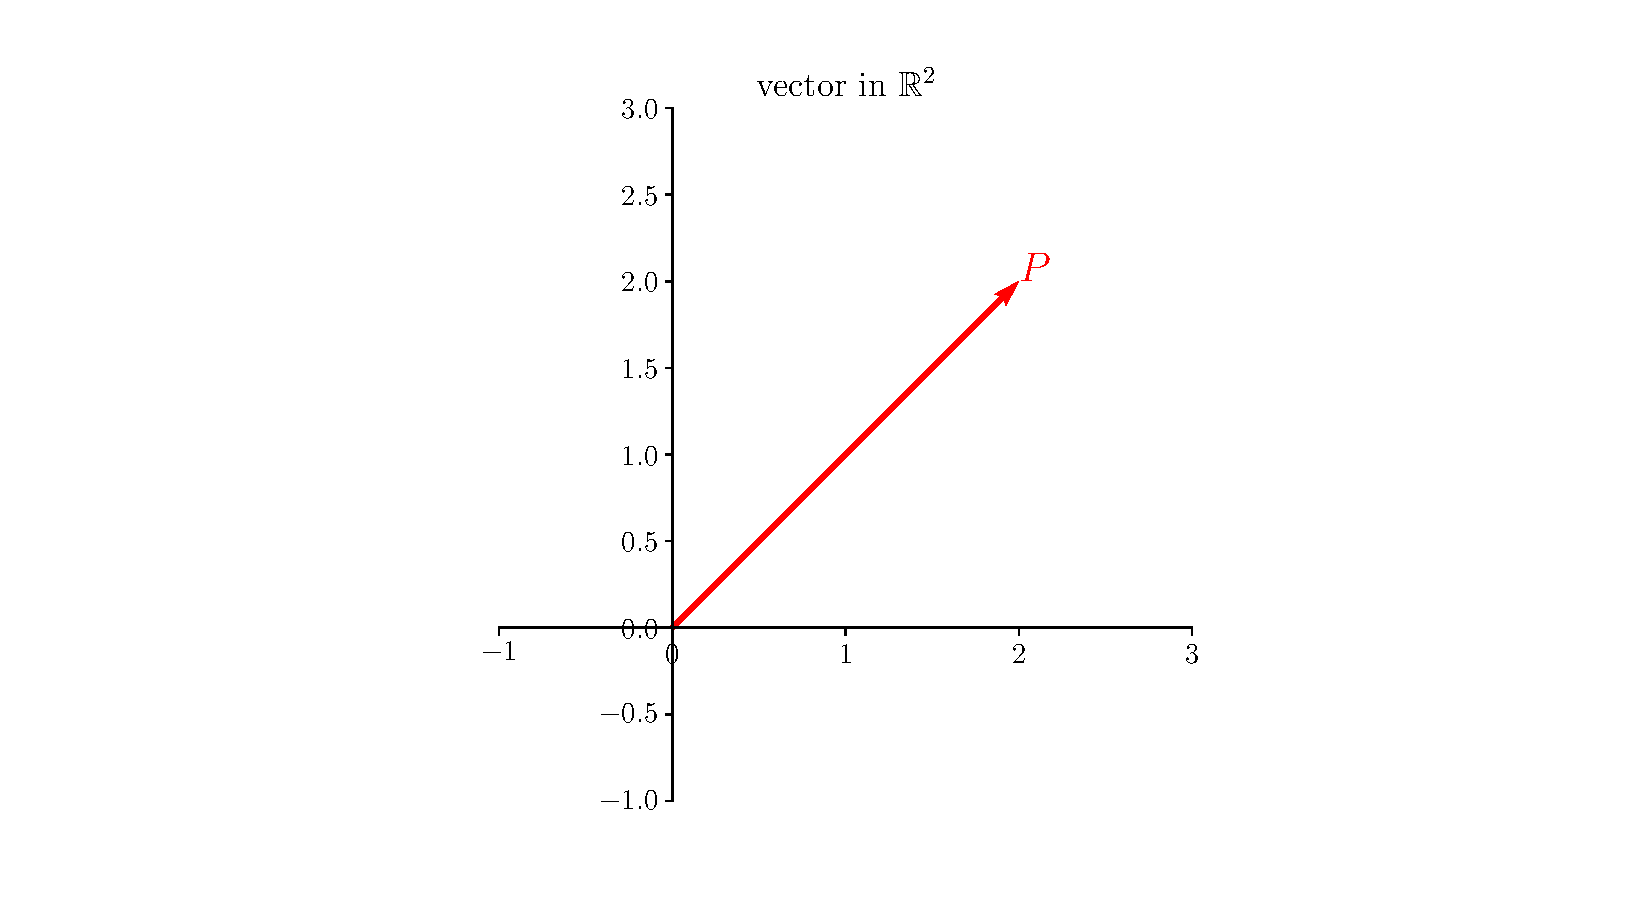
\includegraphics[width=0.5\textwidth]{eps/VectorInR2.eps}
			% \label{}命令为每个子图添加标签, 方便在正文中引用. 如果你不需要引用的话, 也可以不加这个命令, 写法在下面有: 
			% \label{}命令的{}内第一个{}中的内容fig:subfig1就是你插入的这张子图的标签, 注意每个标签都不能一样, 要用合适的编号去区分, 比如1, 2, 3......
			% \label{}命令中{}内\includegraphics[]{}就是真正插入图片的命令, []中的是图片的一些参数, {}就是图片的相对路径
			% width=0.4\textwidth 就是设置图片的大小, 这里设置的是文档宽度(\textwidth)的0.4倍, 在设置时注意不要超宽, 不然会报错, 大家多设置几个数尝试一下就能理解了
		}
		\subfloat[这两个向量是同一个,因为它们的大小和方向都一样]
		{
			\label{fig:same.vector}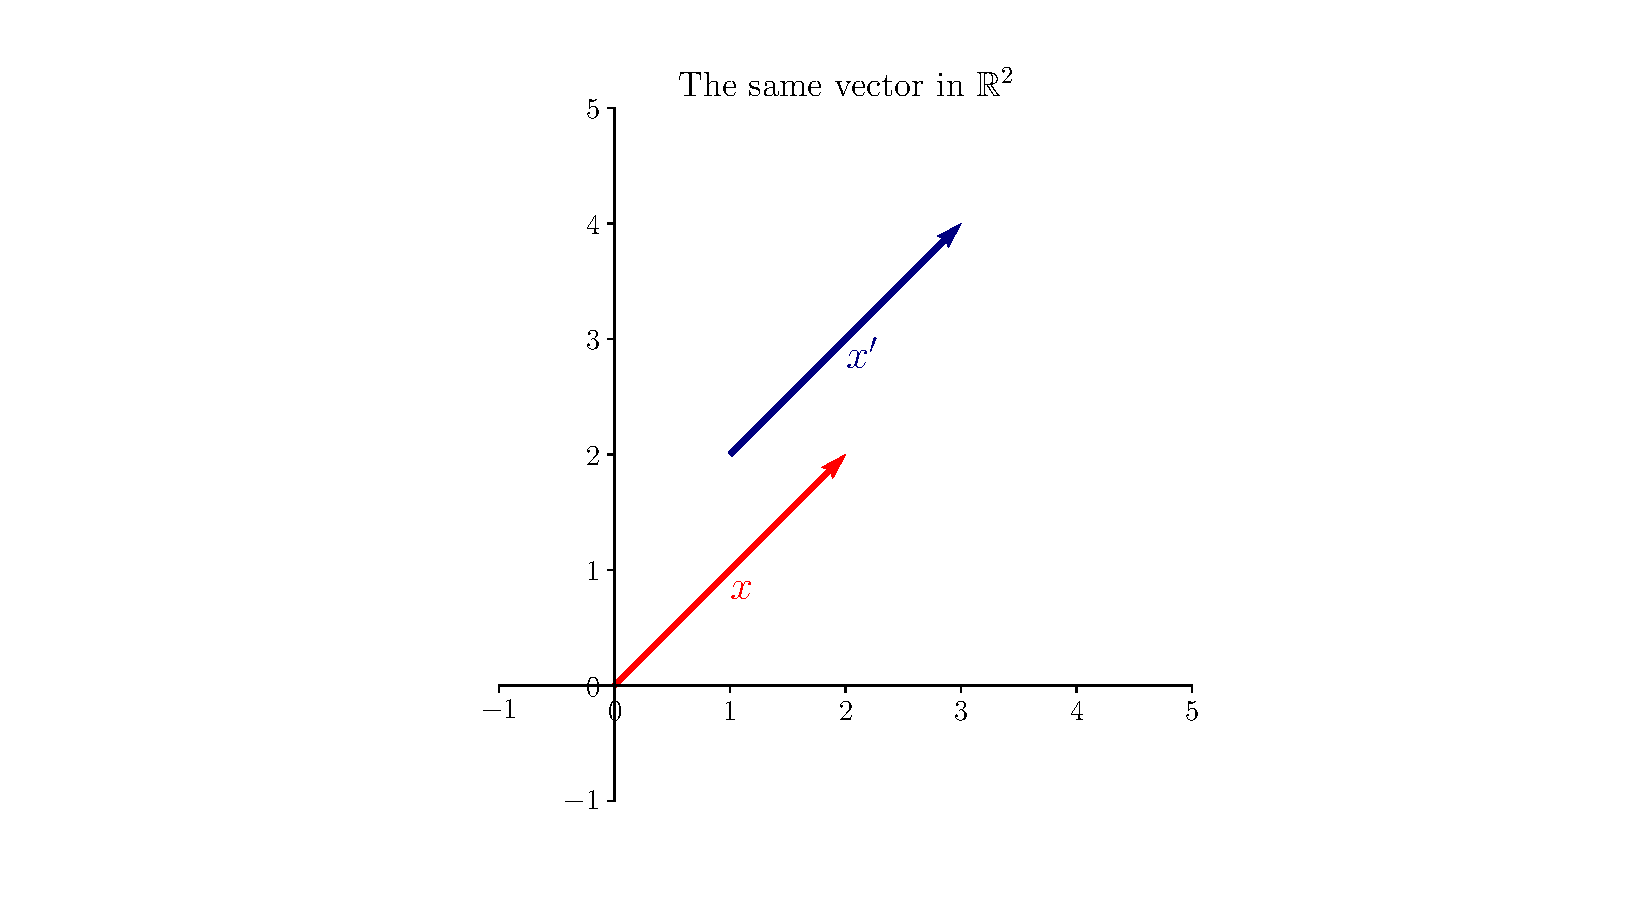
\includegraphics[width=0.5\textwidth]{eps/SameVectorInR2.eps}
		}
		\caption{二维向量}    % 整个图片的说明, 注释写在{}内
		\label{fig:intro.vector}            % 整个图片的标签编号, 注意这里跟子图是一样的道理, 标签不能重复 
\end{figure}

\section{向量的运算法则}
\label{sec:vector.operator}
\subsection{加法}

\begin{definition}{向量的加法}
	\label{def:vectoraddition}
	若$x,y\in \mathbb{F}^n,x=(x_1,x_2,x_3,\cdots,x_n),y=(y_1,y_2,y_3,\cdots,y_n)$则$x+y$定义为$$x+y:=(x_1+y_1,x_2+y_2,x_3+y_3,\cdots x_n+y_n)$$
\end{definition}

实际上两个向量相加,就是将它们元组里面的所有元素依次相加得到一个新的元组。

\begin{ascolorbox1}{思考}
	维度不同的向量是否可以相加?
\end{ascolorbox1}

要解答这个问题,我们需要返回到定义中,我们只定义了维度相同都为$n$的向量相加,并没有定义维度不同的向量相加的情况,所以这是一个未定义的行为;所以下面的对向量的运算均是在同一维度下进行。同理,向量与标量无法相加。

\begin{postulate}
	只有维度相同的向量才能互相相加。
\end{postulate}

同样,向量的加法也满足交换律:
\begin{corollary}
	若$x,y\in \mathbb{F}^n$,则$x+y=y+x$。
\end{corollary}

下面是简单的对此性质的证明(读者不作要求)。

\begin{proof}
	若$x,y\in \mathbb{F}^n,x=(x_1,x_2,x_3,\cdots,x_n),y=(y_1,y_2,y_3,\cdots,y_n)$则$$x+y=(x_1+y_1,x_2+y_2,x_3+y_3,\cdots x_n+y_n)$$根据标量加法的交换律可知
	\begin{equation*}
	x+y=(y_1+x_1,y_2+x_2,y_3+x_3,\cdots y_n+x_n)=y+x \teoe
	\end{equation*}
\end{proof}

如果我们将其反映在二维坐标系上,那应该是这样的
\begin{figure}[htbp]
	\centering
	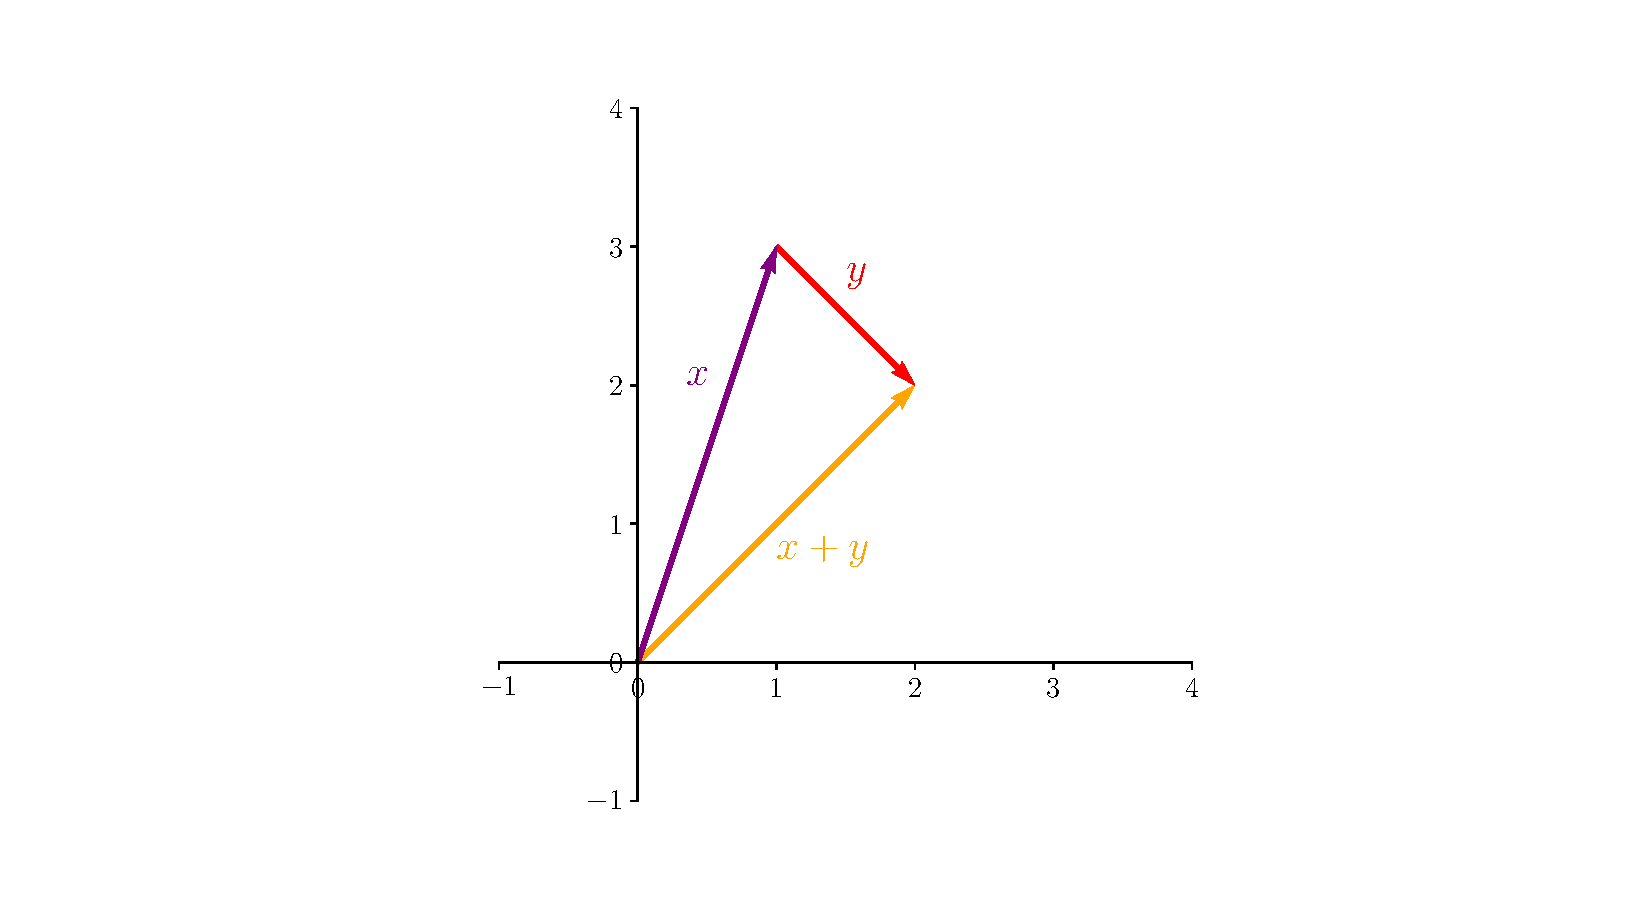
\includegraphics[width=0.7\linewidth]{eps/SumOf2Vectors}
	\caption{平面内两向量之和}
	\label{fig:sumof2vectors}
\end{figure}


\subsection{0 向量}

我们之前说过,向量与标量无法相加,所以在$\mathbb{F}^n$内我们定义$n$维0向量作为加法的单位元,即若$x,y\in \mathbb{F}^n$,$x+y=x$,那么$y$就是0 向量。

\begin{definition}{0 向量}
	若$\alpha,\beta \in \mathbb{F}^n$且$\alpha+\beta = \alpha$,那么$\beta$为空间$\mathbb{F}^n$的单位元,我们将其称为0向量,显然0向量就是一个全是由0组成的$n$元组,记作$\boldsymbol{0}$\footnote{实际上是以粗体形式出现的0},那么$$\boldsymbol{0}=(0,0,0,\cdots,0)$$
\end{definition}

\subsection{加法逆元}

类似于标量加法的$x,y\in \mathbb{C},x+y=0$,其中标量0表示标量加法的单位元,其中$y=-x$,那么在空间$\mathbb{F}^n$中同样表示若$\alpha,\beta \in \mathbb{F}^n,\alpha+\beta=\boldsymbol{0}$,$\beta=-\alpha$表示$\alpha$的加法逆元。

\begin{definition}{加法逆元}
	对于$\alpha \in \mathbb{F}^n$,$\alpha$的加法逆元表示满足下面条件的向量$-\alpha\in \mathbb{F}^n$有$$\alpha+(-\alpha)=\boldsymbol{0}$$换而言之当$\alpha=(a,b,c,d,\cdots)$时,$-\alpha=(-a,-b,-c,-d,\cdots)$
\end{definition}

\subsection{标量乘法}

\begin{definition}{向量的标量乘法}
	\label{def:facmul}
	若标量$\lambda \in \mathbb{F}$,其对一个向量$x=(x_1,x_2,x_3,\cdots,x_n)$的乘积满足以下的运算法则$$\lambda(x_1,x_2,x_3,\cdots,x_n):=(\lambda x_1,\lambda x_2,\lambda x_3,\cdots,\lambda x_n)$$
\end{definition}

实际上如图\ref{fig:mulfsn}所示,向量的标样乘法从$\mathbb{R}^2$的几何意义来看表示的是向量长度的缩放倍率。例如$x=(1,2)$那么$2x=(2,4)$.

\begin{figure}[htbp]
	\centering
	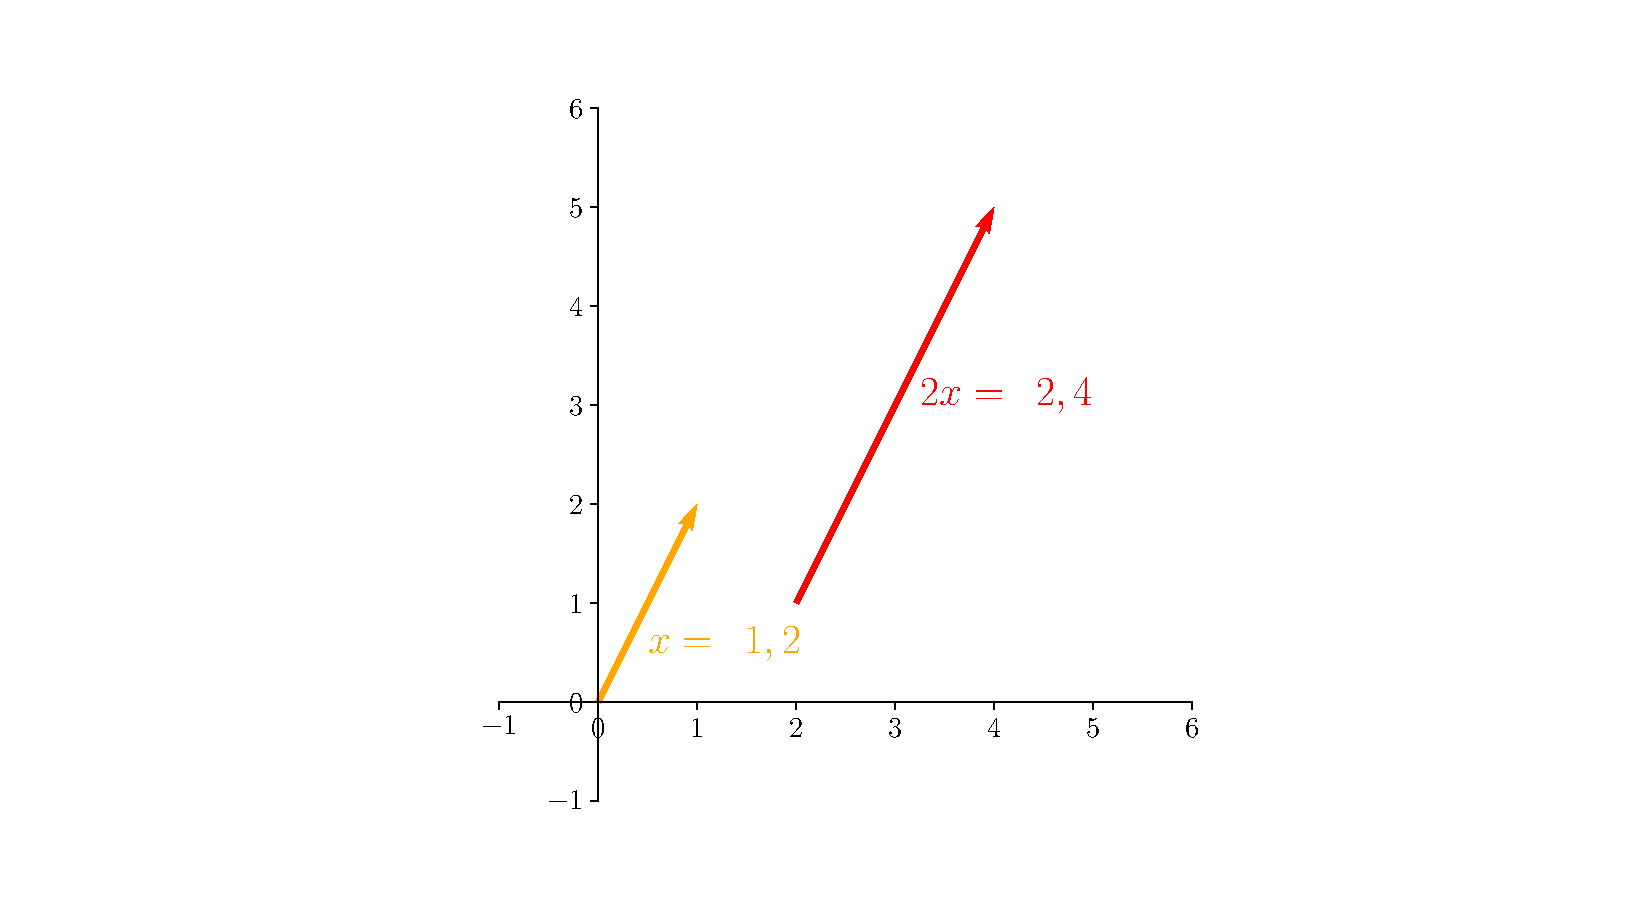
\includegraphics[width=0.7\linewidth]{figure/eps/MulFSn}
	\caption{向量长度的缩放倍率}
	\label{fig:mulfsn}
\end{figure}

同时,向量的标量乘法满足标量结合律。
\begin{corollary}
	若$a,b\in \mathbb{F},x\in \mathbb{F}^n$,满足$(ab)x=a(bx)$。
\end{corollary}

至此,我们对向量的运算法则做一个总结,我们目前只定义了2种运算法则,一种是向量和,另一种是标量积,下面我们会用这两种运算讲解一个特殊的集合,使得这个集合由这两部分构成。

\begin{example}
	已知$x\in \mathbb{R}^4$且满足$(1,1,4,-5)+2x=(5,1,-4,1)$,求$x$。
	\tcblower
	\textcolor{purple}{\textbf{解}}:等式两边同时加上$(1,1,4,-5)$的逆元$(-1,-1,-4,5)$可得$$2x+(0,0,0,0)=(5,1,-4,1)+(-1,-1,-4,5)=(4,0-8,6)$$设$x=(a,b,c,d)$可得$$(2a,2b,2c,2d)=(4,0,-8,6)$$由此可以得到方程组$$\left\{\begin{matrix} 
		2a=4 \\
		2b=0 \\
		2c=-8 \\
		2d=6
	\end{matrix}\right. $$所以可得$x=(2,0,-4,3)$
\end{example}

读者平时在作业的时候无需大费周章地严格用定理来写题目,如果你熟练的话可以直接自己写一个关于向量的减法法则(实际上就是加法法则的逆运算)来做题。

\section{线性空间$\mathbb{R}^2$与$\mathbb{R}^3$}
\subsection{线性空间}
\label{subsec:linearSpace}
如果要刻画线性空间,我们先从空间说起。

前文我们提到了``空间$\mathbb{F}^n$'',那么我们可以在此断章取义地说,空间就是一个集合,而线性空间是一个特殊的集合,我们给它一个符号$V$来表示。

下面给出定义来描述线性空间特殊的地方,线性空间$V$是一个带有加法和标量乘法的集合,下面我们将前面的向量的运算法则抽象化来定义它们。不过在此之前,我希望和大家来聊一聊一些你可能不是很了解的名词,例如函数(function)。
\begin{definition}{函数(一元)}
	对于任意的非空集合$A,B$,对集合$A$施加一个法则$f$使得$A$中的元素$x$可以转变为集合$B$中的元素$y$,记作$f(x)$或$f: A\rightarrow B$,即$y=f(x)$。
\end{definition}

上面讲述了函数的一般情形,那就是一元函数;一元函数有一个显著的特点,就是``输入一个元素并输出一个元素'',当然还有多元函数,下面请读者思考。

\begin{ascolorbox1}{思考}
	两个可以相加的元素进行加法运算,这是一种函数吗?
\end{ascolorbox1}

回答是肯定的,只不过这就不是一元函数了,这是二元函数,即``输入两个元素并输出一个元素'',翻译成数学的符号语言可以是:若$a,b\in A$则$f(a,b):=a+b$。同理,如果我们将集合内的元素特殊化为一种向量,那就是若$a,b\in \mathbb{F}^n$则$f(a,b):=a+b$。

那我们回到线性空间上来,如果一个集合$V$满足下面这一些条件的我们称其为线性空间\footnote{有些教材会叫做向量空间}。

\begin{definition}{线性空间上的加法与标量乘法}
	若集合$V$与数集$\mathbb{F}$满足以下的性质,则称$V$为$\mathbb{F}$上的线性空间:
	\begin{enumerate}
		\item $V$上的加法是一个函数使得任意一对$u,v \in V$经过法则$f(u,v)=u+v$转变为$V$中的另一个元素,这说明了$u+v\in V$。
		\item $V$上的标量乘法是一个函数使得任意一个$\alpha \in \mathbb{F}$和$u\in V$经过法则$f(u)=\alpha u$转变为$V$中的另一个元素,这说明了$\alpha u \in V$。
	\end{enumerate}
\end{definition}

根据的定义,线性空间$V$具有如下的性质:

\begin{definition}{线性空间的性质}
	\label{linear.space.sit}
	线性空间就是带有加法和标量乘法的集合$V$,满足如下的性质:
	\begin{itemize}
		\item 交换性(commutativity):对于所有的$u,v\in V$都有$u+v=v+u$;
		\item 结合性(associativity):对于所有的$u,v,w \in V$和$a,b\in \mathbb{F}$都有$(u+v)+w=u+(v+w)$和$(ab)v=a(bv)$;
		\item 加法单位元(additive identity):存在$\boldsymbol{0}\in V$使得对于所有的$v\in V$都有$v+\boldsymbol{0}=v$;
		\item 加法逆元(additive inverse):对于每一个$v\in V$都存在$w\in V$使得$v+w=\boldsymbol{0}$;
		\item 乘法单位元(multiplicative identity):对于所有的$v\in V$都存在$w\in V$使得$v+w=0$;
		\item 分配性质(distributive properties):对于所有的$a,b \in \mathbb{F}$和$u,v \in V$都有$a(u+v)=au+av$和$(a+b)v=av+bv$。
	\end{itemize}
\end{definition}

\begin{ascolorbox1}{思考}
	空集可以是线性空间吗?
\end{ascolorbox1}

答案为不是,因为空集$A$它不存在单位元$\boldsymbol{0}\in A$所以并不能是线性空间,此外,需要注意的是我们一般会说$V$是$\mathbb{F}$上的线性空间而不会直接说$V$是线性空间,因为我们在定义线性空间的时候,依赖了$\mathbb{F}$这个标量数集。

如之前所承诺的,下面给出向量的定义。

\begin{definition}{向量}
	线性空间中的元素称为向量。
\end{definition}

读者可能会觉得这样给出会有些突然,我们不妨反过来看看向量作为线性空间$V$的元素,是否满足定义\ref{linear.space.sit}的6个条件,然后与读者高中所学的向量的特性对比,发现是否吻合。如果读者觉得这样做还是太抽象,我们不妨研究一下在线性空间$\mathbb{R}^2$与$\mathbb{R}^3$中向量的相关图形表现。

\subsection{直线,平面与三维空间上的向量}

向量同时具有长度和方向两种特性,如果我们在$\mathbb{R}^2$上绘制平面直角坐标系来图像化向量这一个概念的话,向量就是一个有向箭头,由起点和终点构成,若一个有向箭头的起点为$P$,终点为$Q$,我们将此有向箭头\footnote{向量与有向箭头的区别在于,长度相同且方向相同的有向箭头,可以有很多个表示,如图\ref{fig:same.vector}所示,而这两个有向箭头表示的向量是同一个。不过,通常而言,该有向线段也可直接称为向量}记为$\overrightarrow{PQ}$。若$a\in \mathbb{R}^2,a=\overrightarrow{PQ}$,则向量$a$的长度为线段$PQ$的长度,记作$\left \| a \right \| $。

\begin{definition}{$\mathbb{R}^2$上向量的长度}
	\label{def:lengthOfVec}
	若$x\in \mathbb{R}^2$且$x=(x_1,x_2)$,则$x$的长度$\left \| x \right \| $为$$\left \| x \right \| := \sqrt{x_1^2+x_2^2}$$
\end{definition}

\begin{example}
	已知$a,b\in \mathbb{R}^2$,点$O$为平面直角坐标系的原点,$P_1,P_2$分别为一条线段的两个端点,$M$为该线段的重点,其中$a=\overrightarrow{OP_1},b=\overrightarrow{OP_2}$,求$\overrightarrow{OM}$。
	\tcblower
	\textcolor{purple}{\textbf{解}}:在长度上$\left \| \overrightarrow{P_1M} \right \|=\left \| \overrightarrow{MP_2} \right \|$且在同一条直线上,所以$\overrightarrow{P_1M}=\overrightarrow{MP_2}$,根据向量的加法法则有$$\overrightarrow{OM}=\overrightarrow{OP_1}+\overrightarrow{P_1M},\overrightarrow{OM}=\overrightarrow{OP_2}-\overrightarrow{P_1M}$$前后两式相加可得$$\overrightarrow{OM}=\frac{a+b}{2}$$
\end{example}

此外由于向量具有方向性,且可以随处移动,由此我们也可以由此性质确定$\mathbb{R}^2$和$\mathbb{R}^3$空间中直线的方向并确定直线的方程。

\begin{definition}{直线的方向向量}
	空间直线的方向用一个与该直线平行的有向箭头表示,该有向箭头所表示的向量即为空间直线的方向向量。
\end{definition}

\begin{figure}[htbp]
	\centering
	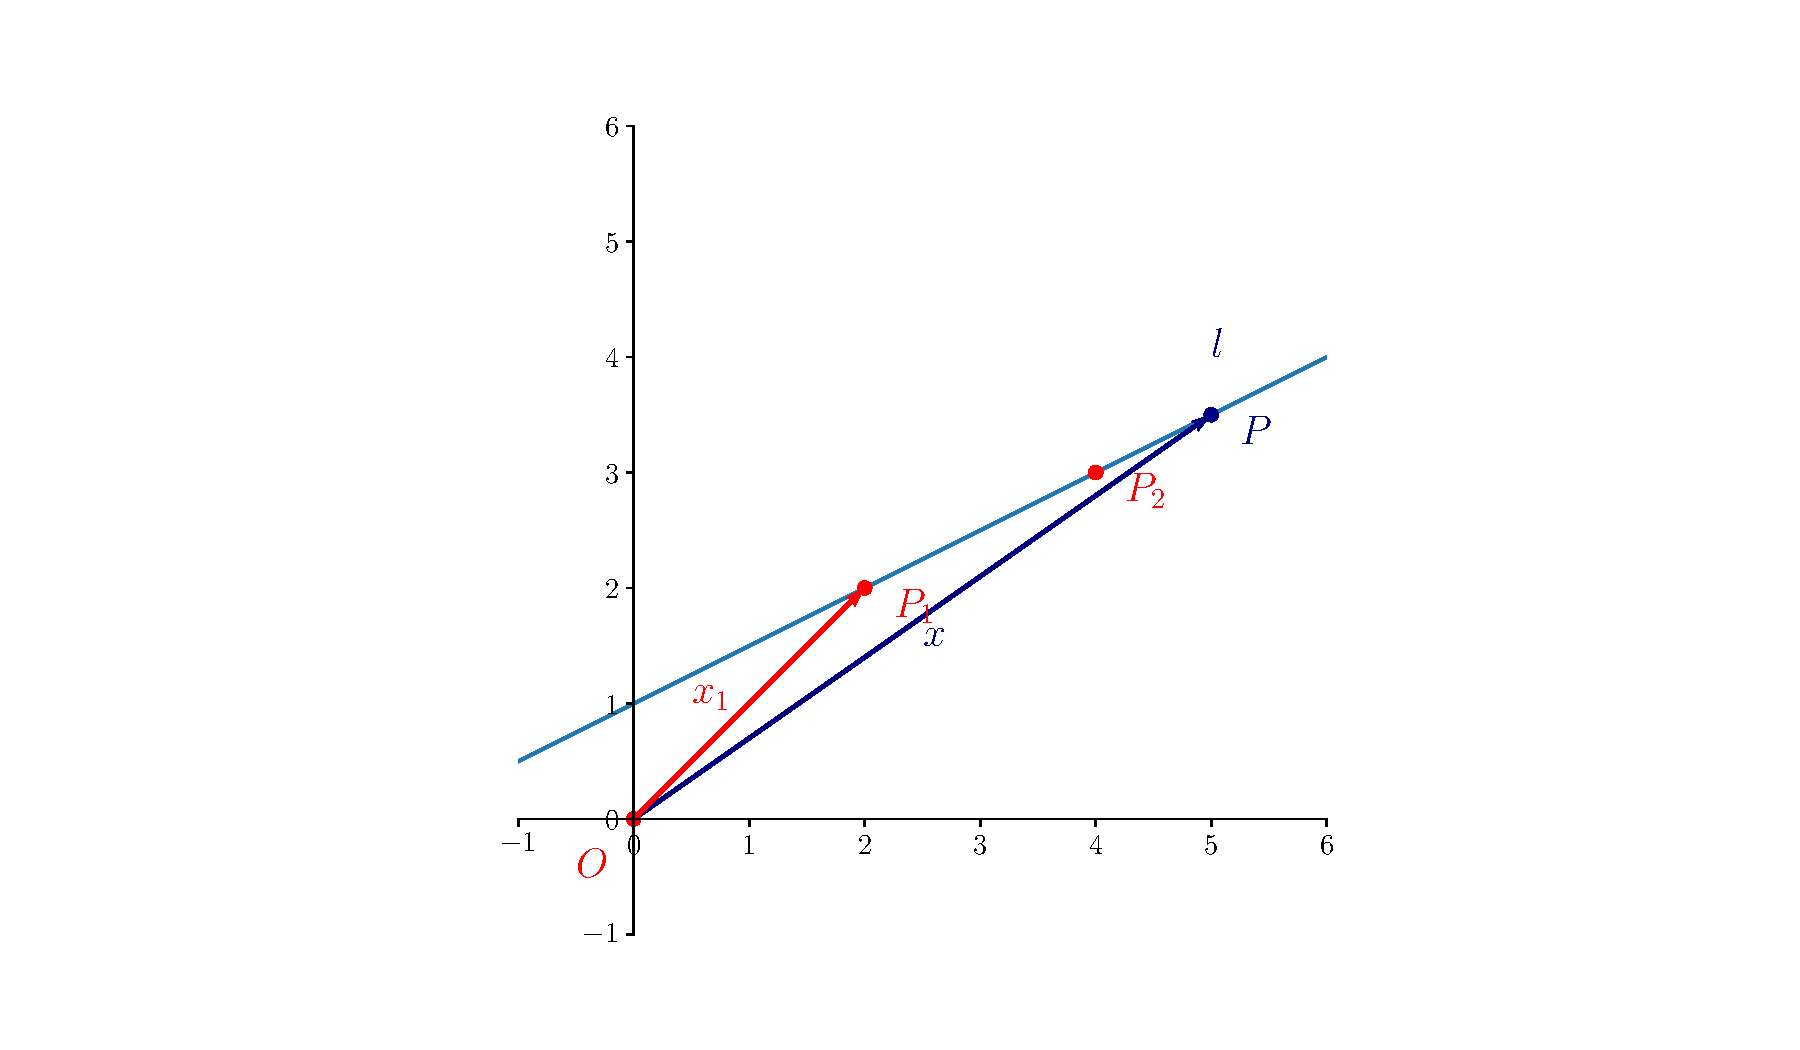
\includegraphics[width=0.7\linewidth]{figure/eps/LineAndVector2d}
	\caption{方向向量与直线方程}
	\label{fig:lineandvector2d}
\end{figure}

如图\ref{fig:lineandvector2d}所示,$P_1$和$P_2$都在直线$l$上,设$x,x_1\in \mathbb{R}^2,x=\overrightarrow{OP},x_1=\overrightarrow{OP_1}$,有向箭头$\overrightarrow{P_1P_2}$在直线$l$上,若向量$a\in \mathbb{R}^2$满足$a=\overrightarrow{P_1P_2}$,则该向量$a$是这条直线的方向向量。

既然知道了直线的方向向量和$O$到直线上某一点的有向箭头所表示的向量,我们就可以建立一个等式来唯一确定一条直线,设$t\in \mathbb{R}$,那么对于任意处于直线上的$P$点,总存在$t$使得$x=\overrightarrow{OP}$满足$$x=x_1+ta$$如果我们设直线上的$P$点坐标为$(x,y)$那么$x=(x,y)$设$P_1$的坐标是$(x_1,y_1)$,$P_2$的坐标是$(x_2,y_2)$,于是乎$a=(x_2-x_1,y_2-y_1)$,由$x=x_1+ta$并代入坐标,根据向量的加法与标量乘积的运算定理,我们可以得到下面的式子$$\left\{\begin{matrix} 
	x-x_1=t(x_2-x_1) \\  
	y-y_1=t(y_2-y_1)
\end{matrix}\right. $$所以我们可以得到这就是经过$P_1$和$P_2$两点的参数方程,如果要进一步往下化简的话,我们可以得到$$\frac{x-x_1}{x_2-x_1}=\frac{y-y_1}{y_2-y_1}$$

\begin{example}
	求二维空间$\mathbb{R}^2$内直线方程$3x+4y-5=0$的一个方向向量。
	\tcblower
	\textcolor{purple}{\textbf{解}}:设$P_1,P_2$点坐标分别为$(x_1,y_1),(x_2,y_2)$,则$a\in \mathbb{R}^2,a=\overrightarrow{P_1P_2}$为其一个方向向量,令$x_1=0$则$\displaystyle y_1=\frac{5}{4}$,$\displaystyle \overrightarrow{OP_1}=\left( 0,\frac{5}{4} \right)$,令$y_2=0$则$\displaystyle x_2=\frac{5}{3}$,$\displaystyle \overrightarrow{OP_2}=\left(\frac{5}{3},0\right)$,$\overrightarrow{P_1P_2}=\overrightarrow{OP_2}-\overrightarrow{OP_1}$所以该直线的一个方向向量为$\displaystyle \left( \frac{5}{3},-\frac{5}{4} \right) $
\end{example}

接下来我们将维度扩展到三维空间$\mathbb{R}^3$内,依然有$$x=x_1+ta$$由此如果$P_1$与$P_2$的坐标分别为$(x_1,y_1,z_1)$和$(x_2,y_2,z_2)$,我们将会得到下面的等式$$\frac{x-x_1}{x_2-x_1}=\frac{y-y_1}{y_2-y_1}=\frac{z-z_1}{z_2-z_1}$$这就是空间内的直线方程(实际上就是两个一次方程)

\begin{example}
	求三维空间$\mathbb{R}^3$内直线方程$$\left\{\begin{matrix} 
		x+y+z=3 \\  
		x+2y+3z=6
	\end{matrix}\right. $$的一个方向向量。
	\tcblower
	\textcolor{purple}{\textbf{解}}:设$P_1,P_2$点坐标分别为$(x_1,y_1,z_1),(x_2,y_2,z_2)$,则$a\in \mathbb{R}^3,a=\overrightarrow{P_1P_2}$为其一个方向向量,令$x_1=1$则$\displaystyle y_1=1,z_1=1$,$\displaystyle \overrightarrow{OP_1}=\left( 1,1,1 \right)$,令$x_2=0$则$\displaystyle y_2=3,z_2=0$,$\displaystyle \overrightarrow{OP_2}=\left(0,3,0\right)$,$\overrightarrow{P_1P_2}=\overrightarrow{OP_2}-\overrightarrow{OP_1}$所以该直线的一个方向向量为$\displaystyle \left( -1,2,-1 \right) $
\end{example}

同样的,根据两条相交直线可以确定平面,如果我们使用向量来考虑$\mathbb{R}^3$上的平面的话,通过两个不互相平行的非零向量和一点也能确定一个平面,如图\ref{tikz:space.face}所示。

\begin{figure}[htbp]
	\centering
	\tdplotsetmaincoords{60}{70}

\begin{tikzpicture}[yscale=1.5,xscale=1.5,line width=0.8pt,tdplot_main_coords]
	\coordinate (A) at (0,0,0);
	\coordinate (B) at (4,0,0);
	\coordinate (C) at (4,3,0);
	\coordinate (D) at (0,3,0);
	\coordinate (O) at (0.5,0.5,2);
	
	\coordinate (P) at (3.5,2.5,0);
	\coordinate (P1) at (0.5,0.5,0);
	\coordinate (P2) at (2.5,0.5,0);
	\coordinate (P3) at (0.5,2,0);
	\coordinate (P3t) at (0.5,2.5,0);
	\coordinate (P2t) at (3.5,0.5,0);
	
	
	\draw[rounded corners=0.05pt](A)--(B)--(C)--(D)--(A);
	
	\draw[->,>=Stealth](O)node[above=3.5pt,right=3pt]{$O$}--(P)node[above=2.5pt,right=2.5pt]{$P$};
	\draw[->,>=Stealth](O)--(P1)node[above=2.5pt,left=1.5pt]{$P_1$};
	\draw[->,>=Stealth](P1)--(P2)node[above=2.5pt,right=2.5pt]{$P_2$};
	\draw[->,>=Stealth](P1)--(P3)node[right=2.5pt]{$P_3$};
	\draw[dashed](P1)--(P3t)--(P)--(P2t)--(P1);
	\draw[->,>=Stealth](P1)--(P);
	%\draw(P)node[above=3.5pt,right=3pt]{$P$};
\end{tikzpicture}
	\caption{$P$在平面上}
	\label{tikz:space.face}
\end{figure}

类比于直线的向量表示,设向量$x,x_1,a,b\in \mathbb{R}^3$,$P,P_1,P_2,P_3$点在平面上,令$x=\overrightarrow{OP},a=\overrightarrow{P_1P_2},b=\overrightarrow{P_1P_3},x_1=\overrightarrow{OP_1}$,设$t,s\in \mathbb{R}$,对于任意处于平面上的$P$点,总存在$t,s$使得$x=\overrightarrow{OP}$满足$$x=x_1+ta+sb$$由于过空间内不在同一直线上的三个点写方程很复杂,限于篇幅结构笔者不再详细介绍推导过程\footnote{可能会有读者会说平面的点法式方程,我知道学霸读者很多,但是笔者需要考虑给入门的选手讲清楚这些,后面我们会慢慢接触它们,请不要着急。}。不过笔者在此给出平面方程的一般形式(只有一个等式)。$$ax+by+cz+d=0,a,b,c,d\in \mathbb{R}$$

\subsection{其他线性空间}

上面我们讲了$\mathbb{R}^2$和$\mathbb{R}^3$是一种线性空间,更一般的例子就是$\mathbb{R}^n$,再一般的例子就是$\mathbb{C}^n$。

\begin{definition}{实线性空间与复线性空间}
	\begin{itemize}
		\item $\mathbb{R}$ 上的线性空间称作实线性空间。
		\item $\mathbb{C}$ 上的线性空间称作复线性空间。
	\end{itemize}
\end{definition}

除此之外,还有多项式空间也是线性空间,下面给出定义。

\begin{definition}
	所有次数不超过$n$的实系数多项式的集合,记作$P_n$。
\end{definition}

$P_n$ 中的元素是形如 $p(x) = a_0 + a_1 x + a_2 x^2 + \cdots + a_n x^n$ 的多项式,其中 $a_0, a_1, \dots, a_n \in \mathbb{R}$,接下来我们来验证$P_n$是线性空间。

\begin{corollary}
	$P_n$是$\mathbb{R}$或$\mathbb{C}$上线性空间。
\end{corollary}

下面给出证明(读者并不要求)

\begin{proof}
	验证加法,两个多项式相加是按系数相加,例如:$$p(x) + q(x) = (a_0 + b_0) + (a_1 + b_1)x + \cdots + (a_n + b_n)x^n$$可以得到他们的和依然是多项式。其次验证标量乘法,标量 $c \in \mathbb{R}$ 与多项式 $p(x)$ 的乘积是$$c p(x) = c a_0 + c a_1 x + \cdots + c a_n x^n$$所得的结果依然是多项式,若$P(x)=0$,代表的是该线性空间的零向量,满足线性空间的所有公理。$\square$
\end{proof}

\begin{ascolorbox1}{思考}
	你能不能举出其他的一些例子表示线性空间?
\end{ascolorbox1}

\section{子空间}

\subsection{子空间(subspace)的定义}

\begin{definition}
	如果$V$的子集$U$也是线性空间,则称$U$是$V$的子空间。
\end{definition}

例如$U=\left\{ (x_1,x_2,0) \mid x_1,x_2 \in \mathbb{R} \right\}$是$\mathbb{R}^3$的子空间。需要要注意的是,线性空间的子集也得是线性空间所以才能是子空间,所以请读者思考下面的一个问题。

\begin{ascolorbox1}{思考}
	$U=\left\{ (x_1,x_2,1) \mid x_1,x_2 \in \mathbb{R} \right\}$是否是$\mathbb{R}^3$的子空间?
\end{ascolorbox1}

答案为不是,因为它不满足$\boldsymbol{0}\in U$,根本就不是线性空间,所以不是$\mathbb{R}^3$的子空间。除此之外,子空间需要满足下面的情况(也就是说,也需要满足作为线性空间的条件)。

\begin{corollary}
	当且仅当 $V$ 的子集 $U$ 满足以下三个条件时,$U$ 是 $V$ 的子空间。
	\begin{itemize}
		\item 存在加法单位元$\boldsymbol{0}\in U$;
		\item 对于加法封闭,即$v,w\in U$满足$v+w\in U$;
		\item 对于标量乘法封闭,即$\lambda \in \mathbb{F},v\in U$满足$\lambda v\in \mathbb{F}$。
	\end{itemize}
\end{corollary}

\begin{ascolorbox1}{思考}
	若集合$U=\left\{ (x_1,x_2,0) \mid x_1,x_2 \in \mathbb{R} \right\}$,集合$T=\left\{ (0,0,x_3) \mid x_3 \in \mathbb{R} \right\}$,$T\cup U$是否是$\mathbb{R}^3$的子空间?
\end{ascolorbox1}

答案为不是,因为它不满足对于加法封闭,取$u\in U,u=(1,1,0),t \in T,t=(0,0,1)$,$u+t=(1,1,1) \notin U\cup T$,所以不是$\mathbb{R}^3$的子空间。

\subsection{子空间之和}

为了更深入了解线性空间以及知识完整性,下面讲解子空间和的概念。

\begin{definition}{子空间的和}
	子空间的和是有其所有元素可能的和所构成的集合,其结果仍是子空间。若$V_1,V_2,V_3,\cdots,V_m$是$V$的子空间,则子空间的和$V_s$记作$$V_s=V_1+V_2+V_3+\cdots+V_m=\sum_{i=1}^{m}V_i $$或者说来$$V_s=\sum_{i=1}^{m}V_i =\left\{ \sum_{i=1}^{m}v_i \mid i\in \mathbb{N}^+,v_i \in V_i \right\}$$
\end{definition}

不要被定义上的Sigma符号吓跑了,实际上就是分别任意两个属于不同子空间的元素相加后的新元素所构成的空间,例如子空间$V_1=\left\{ (x_1,x_2,0)\mid x_1,x_2\in \mathbb{R} \right\}$和$V_2=\left\{ (0,x_3,x_4)\mid x_3,x_4\in \mathbb{R} \right\}$,则$V_1,V_2$子空间的和是$\mathbb{R}^3$,即$\mathbb{R}^3$中所有的元素$r$均存在$t,s\in \mathbb{R}$使得$v_1\in V_1$,$v_2\in V_2$满足$$r=tv_1+sv_2$$

所以可以记作$\mathbb{R}^3=V_1+V_2$。

上面讲了子空间的和,请读者先思考子空间的和与子空间的并的区别。

\begin{ascolorbox1}{思考}
	子空间的并是否一定是子空间?在什么情况下子空间的并是子空间?
\end{ascolorbox1}

首先回答第一个,子空间的并不一定是子空间,如上面的一个思考$T\cup U$一样,$U,T$均为$\mathbb{R}^3$的子空间,但是我们证明了它们的并集不是子空间。对于第二个问题,首先我们考虑$V$子空间$T$和$U$,如果$T$是$U$的非空子集(思考为什么非空?),那么$T \cup U=U$是子空间显然成立,若$T$不是$U$的非空子集,设$t\in T,u\in U$由子空间的性质应有$t+u$属于$V$,即$t+u$可能属于$T$也可能属于$U$。但是若$t+u$属于$T$,而根据封闭性$u=(t+u)-t$也应当属于$T$,$t+u$和$u$都是子空间$T$的元素,所以与``若$T$不是$U$的非空子集''的设定不符。

\begin{corollary}
	两个子空间的并集是子空间,当且仅当其中一个包含于另一个。
\end{corollary}

\subsection{直和}

首先我们回顾一下笛卡尔积\footnote{笛卡尔积的另一个名称叫做直积,和本部分的直和的运算方式有关联。},如果读者已经忘记了的话请阅读定义\ref{def:dicar},我们了解到$\mathbb{R}^3$空间由$\mathbb{R}\times\mathbb{R}\times\mathbb{R}$通过笛卡尔积生成。而直和也是生成生成空间的一种方式,是一种特殊的子空间之和。

\begin{definition}{直和(direct sum)}
	设$V_1,V_2,V_3,\cdots,V_m$是$V$的子空间,如果$V_1+V_2+V_3+\cdots+V_3$中的每个元素都能用$\sum_{i=1}^{m}v_i ,v_i\in V_i$唯一地表示出来,则称子空间之和$\sum_{i=1}^{m}V_i $为直和,可写作$$V=V_1\oplus V_2\oplus V_3\oplus \cdots \oplus V_m$$
\end{definition}

例如$A=\left\{ (x,y,0)\mid x,y \in \mathbb{R} \right\},B=\left\{ (0,0,z)\mid z\in \mathbb{R} \right\}$,则$\mathbb{R}^3=A \oplus B$;而$A=\left\{ (x,y,z)\mid x,y,z \in \mathbb{R} \right\},B=\left\{ (0,0,z)\mid z\in \mathbb{R} \right\}$,则$\mathbb{R}^3\neq A \oplus B$。

\begin{corollary}
	$U$ 和 $W$ 是 $V$ 的子空间且$V=U\oplus W$,当且仅当$W\cap U=\left\{ 0 \right\}$。
\end{corollary}

接下来我们继续研究构建线性代数的基本内容,即向量与空间的关系。

\section{张成空间与线性相关性}

\subsection{线性组合与张成空间}

一组向量进行标量乘法后相加形成的一个向量,称作该向量的线性组合。

\begin{definition}{线性组合(linear combination)}
	给定向量集合 $\{v_1, v_2, \dots, v_k\}$ 和标量集合 $\{c_1, c_2, \dots, c_k\}$,向量 $v$ 的线性组合表示为:$$v = c_1 v_1 + c_2 v_2 + \dots + c_k v_k$$其中,$c_1, c_2, \dots, c_k$ 称为组合系数。
\end{definition}

通过一组向量的线性组合所产生的向量能表示的空间是这个向量的张成空间,下面给出定义。

\begin{definition}{张成空间(span)}
	给定向量集合 $ S = \{v_1, v_2, \dots, v_k\} $(其中 $ v_i $ 是线性空间 $ V $ 中的向量),这些向量的张成空间是所有可能的线性组合构成的集合,记作:$$\text{Span}(S) = \{ c_1 v_1 + c_2 v_2 + \dots + c_k v_k \mid c_1, c_2, \dots, c_k \in \mathbb{F} \}$$如果$V=\text{Span}(S)$,则称向量集合$S$张成\footnote{这里的张成是动词。}空间$V$。
\end{definition}

例如$(1,2,4) \in \text{Span}(\left\{ (1,0,0),(0,1,2) \right\})$因为存在线性组合使得$(1,2,4)=(1,0,0)+2(0,1,2)$,而$(1,2,5) \notin \text{Span}(\left\{ (1,0,0),(0,1,2) \right\})$因为不存在线性组合使得$(1,2,5)=\lambda (1,0,0)+\beta (0,1,2)$。

再有例子$\mathbb{R}^3=\text{Span}(\left\{ (1,0,0),(0,1,0),(0,0,1) \right\})$,因为任何一个$v\in \mathbb{R}^3$都可以由$\left\{ (1,0,0),(0,1,0),(0,0,1) \right\}$的线性组合构成。

\begin{corollary}
	张成空间$\text{Span}(S)$是包含向量$S$空间的子空间。
\end{corollary}

不要笑!可能这个概念对读者来说就像$2+2=4$一样简单,这个推论是显然的,张成空间是子空间,但是我们还是来证明它。

\begin{proof}
	对于$V=\text{Span}(S),S=\left\{ v_1,v_2,v_3,\cdots,v_n \right\}$,有加法单位元$\boldsymbol{0}\in V$,在此空间$V$中$$\boldsymbol{0}=\sum_{i=1}^{n}(0v_i) $$在空间$V$中满足在加法封闭$$\sum_{i=1}^{n}a_iv_i+ \sum_{i=1}^{n}c_iv_i=\sum_{i=1}^{n}(a_i+c_i)v_i$$也满足在标量乘法下封闭$$\lambda \sum_{i=1}^{n}a_iv_i= \sum_{i=1}^{n}\lambda a_iv_i$$所以张成空间$\text{Span}(S)$是包含向量$S$空间的子空间。
	\begin{flushright}
		$\square$
	\end{flushright}
\end{proof}

\subsection{线性相关性}

\label{subsec:LinearDependence}
下面我们给出线性代数的一个关键定义,从此往后,我们线性代数研究的内容就是有限维的线性空间。

\begin{definition}{有限维线性空间}
	线性空间如果可以由其空间内的有限个向量张成,则这个线性空间是有限维的。
\end{definition}

同时,我们在此基础上研究线性相关性;设$v_1,v_2,v_3,\cdots,v_n \in V$且$v \in \text{Span}(V)$,根据张成空间的定义我们有$a_1,a_2,a_3,\cdots,a_n \in \mathbb{F}$使得$$v = \sum_{i=1}^{n}a_iv_i =a_1v_1+a_2v_2+a_3v_3+\cdots+a_nv_n$$若$v=\boldsymbol{0}$,我们有一组显然的结果,即当$a_1=a_2=a_3=\cdots=a_n=0$的时候,$v=\boldsymbol{0}$,然而通常来说,我们可能还会遇到其他的$a_i$组合也可以使得$v=\boldsymbol{0}$,于是我们做出如下定义:

\begin{definition}{线性无关\footnote{有些书中会写成线性独立}(linearly independent)}
	对于向量$v_1,v_2,v_3,\cdots,v_n$如果使得其线性组合$a_1v_1+a_2v_2+a_3v_3+\cdots+a_nv_n=\boldsymbol{0}$的情况只有$a_1=a_2=a_3=\cdots=a_n=0$,则称向量$v_1,v_2,v_3,\cdots,v_n$线性无关。
\end{definition}

\begin{definition}{线性相关(linearly dependent)}
	若一些向量不是线性无关的,就称为线性相关。
\end{definition}

给出例子,向量$(1,0,0),(2,0,0),(0,0,3)$是线性相关的,因为存在$\boldsymbol{0}=2(1,0,0)+(-1)(2,0,0)+0(0,0,3)$而$(1,0,0),(0,2,0),(0,0,3)$是线性无关的,因为只有$a_1=a_2=a_3=0$使得$\boldsymbol{0}=0(1,0,0)+0(0,2,0)+0(0,0,3)$。

\begin{example}
	向量$(2,3,1),(1,-1,2),(7,3,c)$线性相关,求$c$的值。
	\tcblower
	\textcolor{purple}{\textbf{解}}:若三个向量线性相关,则有$\alpha,\beta,\gamma \in \mathbb{R},\alpha (2,3,1)+\beta (1,-1,2)+\gamma (7,3,c)=0$,可得线性方程$$\left\{\begin{matrix} 
		2\alpha +1\beta+7\gamma = 0 \\  
		3\alpha +(-1)\beta+3\gamma=0 \\
		1\alpha +2\beta+c\gamma=0
	  \end{matrix}\right.$$若使得线性方程组有非全为0解,我们任意取$\alpha = 1$,则根据前两个式子可得$$\left\{\begin{matrix} 
		1\beta+7\gamma = -2 \\
		(-1)\beta+3\gamma= -3 
		\end{matrix}\right.$$解其可得$\beta=1.5,\gamma=-0.5$而$\alpha=1$,带入第三式,$1+2\times 1.5-0.5c=0$最终结果为$$c=8$$
\end{example}

\begin{corollary}
	如果一组向量线性相关,那么其中一个向量均可以由其他向量的线性组合表示。
\end{corollary}

\begin{proof}
	一组向量 $v_1, v_2, \dots, v_n$ 是线性相关的,当且仅当存在不全为零的标量 $c_1, c_2, \dots, c_n$,使得:$$c_1 v_1 + c_2 v_2 + \dots + c_n v_n = \mathbf{0}$$由于向量组线性相关,至少存在一个标量 $c_k \neq 0$($1 \leq k \leq n$)而将上述等式中的 $v_k$ 单独移到等式一侧:$$c_k v_k = -c_1 v_1 - c_2 v_2 - \dots - c_{k-1} v_{k-1} - c_{k+1} v_{k+1} - \dots - c_n v_n$$两边同除$c_k$可得$$v_k = -\frac{c_1}{c_k} v_1 - \frac{c_2}{c_k} v_2 - \dots - \frac{c_{k-1}}{c_k} v_{k-1} - \frac{c_{k+1}}{c_k} v_{k+1} - \dots - \frac{c_n}{c_k} v_n$$本题得证。$\square$
\end{proof}

这个例子也说明了线性相关的向量集合张成的空间与其去掉任意一个向量后张成的空间是同一个空间。

此外也有一条重要的结论,若向量集合$V$内的元素线性无关,则$V$中元素的个数不大于张成该空间$U$的向量的个数。举个例子,$\left( 0,0,1 \right)$和$(0,1,0)$在$\mathbb{R}^3$线性无关,而张成$\mathbb{R}^3$的向量可能由$(1,0,0),(0,1,0),(0,0,1)$(或更多其他3个不共面的向量)构成,但是既要线性无关,而且还要张成这个空间的向量集合(下面会给这些向量集合一个名字叫做基)在$\mathbb{R}^3$上为3个\footnote{关于这个推论可能会比较抽象,读者可以回想在高中的学习生活中,通过空间直角坐标系的三个基底可以表示整个空间,缺一不可,且3个不共面的向量都可以成为基底,在后面的学习中,我们会给它一个名词叫做极大线性无关组。}。

根据上述推论我们有 Steinitz 替换定理:

\begin{theorem}{Steinitz 替换定理}
	\label{the:Steinitz}
	一个向量集合 $ A $ 是线性无关的,另一个向量组 $ B $ 生成了 $ A $ 所在线性空间,设 $A,B$ 的向量个数分别为 $s,r$ 则 $s\le r$。
\end{theorem}

这里我们不作证明,但是希望读者能够理解这个定理;例如在线性空间$\mathbb{R}^3$上,我们可以选择3个线性无关向量作为基底,此外也有3个及以上能够张成此空间的向量。\footnote{关于此内容我们会在节\ref{subsec:preRank}详细讲述}

\subsection{基与维数}

通过线性无关和张成空间的两个概念的结合,我们可以得到基的概念。

\begin{definition}{基(basis)}
	若$V$中的一组向量线性无关且能够张成$V$,则称这组向量的集合称作$V$的基。
\end{definition}

所以按照上面的定义,基有两个方面的约束:
\begin{itemize}
	\item 基的选取必须是线性无关的,例如$\left\{ (1,0),(2,0),(0,1) \right\}$不能选为$\mathbb{R}^2$的基,因为$\boldsymbol{0}=-2(1,0)+(2,0)+0(0,1)$,这个例子说明二维平面内的基不能共线。
	\item 基的选取必须能张成选取的空间,例如$\left\{ (1,0,0),(0,1,0) \right\}$不能选为$\mathbb{R}^3$的基,因为它们只能张成\\$\left\{ (x,y,0)\mid x,y \in \mathbb{R} \right\}$,这个例子说明两个不共线的向量只能表示整个平面。
\end{itemize}

集合$\left\{ (1,0,0,\cdots,0),(0,1,0,\cdots,0),(0,0,1,\cdots,0),\cdots,(0,0,0,\cdots,1) \right\}$是$\mathbb{F}^n$的基,它比较特殊,是为$\mathbb{F}^n$的\textbf{标准基}。

\begin{corollary}
	若空间$V$包含向量集合$S=\left\{ v_1,v_2,v_3,\cdots,v_n \right\}$且$S$是空间$V$的基,则仅有唯一的$a_1,a_2,a_3,\cdots \in \mathbb{F}$线性组合表示任意一个$V$的元素$v$,即每个$v\in V$都能唯一地表示成下面的形式:$$v=a_1v_1+a_2v_2+a_3v_3+\cdots+a_nv_n$$
\end{corollary}

\begin{example}
	求$U=\left\{ (a,b,c,d,e)\in \mathbb{R}^5 \mid a=2b,c=4d \right\}$的一个基集合。
	\tcblower
	\textcolor{purple}{\textbf{解}}:子空间 $ U $ 中的向量可以表示为:$$(a, b, c, d, e) = (2b, b, 4d, d, e)$$将向量表示为自由变量的线性组合$$(2b, b, 4d, d, e) = b(2, 1, 0, 0, 0) + d(0, 0, 4, 1, 0) + e(0, 0, 0, 0, 1)$$这表明 $ U $ 中的任意向量都可以由向量组 $ \left\{ (2, 1, 0, 0, 0), (0, 0, 4, 1, 0), (0, 0, 0, 0, 1) \right\} $ 线性表示,因此,子空间 $ U $ 的一个基集合为$$\left\{ (2,1,0,0,0), (0,0,4,1,0), (0,0,0,0,1) \right\}$$
\end{example}

接下来我们引入维数的概念:

\begin{definition}{维数(dimension)}
	有限维线性空间的任意一个基集合元素的个数称为该空间的维数,若$V$是有限维的,那么它的维数记作$\text{dim} V$。
\end{definition}

例如上面的例题所表示,子空间$U$的基向量元素的个数为3,即$\text{dim} U=3$,需要注意的是它虽然在$\mathbb{R}^5$空间内,但是张成它至少只需要3个向量,维度为3而不是5。相当于$\{(1,0,0),(0,1,0)\}$只能张成一个平面,但这个平面是放在立体空间内的。

至此,关于线性空间的内容我们就讲到这里,后面给出一些练习供读者参考。

\section{章节练习}

\subsection{A组}

\begin{reidai}
	求$\displaystyle \left( \frac{-1+\sqrt{3}\mathrm{i}}{2} \right)^3$。
\end{reidai}

\begin{reidai}
	设子空间$$U=\left\{ (x,x,y,y)\mid x,y\in \mathbb{F} \right\},W=\left\{ (x,x,x,y)\mid x,y\in \mathbb{F} \right\}$$求子空间的和$U+W$。
\end{reidai}

\begin{reidai}
	判断$\left\{ (x,y,z) \mid x,y,z\in \mathbb{R},xyz=0 \right\}$是否是$\mathbb{R}^3$的子空间。
\end{reidai}

\begin{reidai}
	写出在$\mathbb{R}^3$中过点$(1,4,1)$且方向向量等于$(2,3,1)$的直线方程。
\end{reidai}

\begin{reidai}
	写出在$\mathbb{R}^3$中的平面$2x-y+3z=1$的一个向量表示。
\end{reidai}

\begin{reidai}
	求$t\in \mathbb{R}$使得${(3,1,4),(2,-3,5),(5,9,t)}$线性相关。
\end{reidai}

\begin{reidai}
	求$\left\{ (x,x,y)\mid x,y \in \mathbb{R} \right\}$的一个基集合。
\end{reidai}

\begin{reidai}
	若子空间$V$的$\text{dim} V=1$,求子空间$V$的一个可能解。
\end{reidai}

\subsection{B组}

\begin{reidai}
	若$a,b\in \mathbb{R}^2$,设$O$是平面直角坐标系的原点,$P_1,P_2$分别为平面上一点,其中$a=\overrightarrow{OP_1}=(x_1,y_1),b=\overrightarrow{OP_2}=(x_2,y_2)$,若直线$OP_1$与直线$OP_2$垂直,求$x_1y_1+x_2y_2$。
\end{reidai}

\begin{reidai}
	若$\text{Span}(\left\{ v_1,v_2,v_3,v_4 \right\})=\left\{ (a,b,b,b,b)\mid a,b \in \mathbb{R} \right\}$,求$\text{Span}(\left\{ v_1-v_2,v_2-v_3,v_3-v_4,v_4 \right\})$。
\end{reidai}

\begin{reidai}
	若$U_1,U_2$是有限维线性空间的子空间,已知$\text{dim}U_1=3,\text{dim}U_2=4,\text{dim}(U_1 \cap U_2)=2$,求$\text{dim}(U_1+U_2)$的值。
\end{reidai}

\begin{reidai}
	若$U_1,U_2$是有限维线性空间的子空间,求证$$\text{dim}U_1+\text{dim}U_2-\text{dim}(U_1 \cap U_2)=\text{dim}(U_1+U_2)$$
\end{reidai}

\begin{reidai}
	设$U,W$是$\mathbb{R}^n$的子空间且$\text{dim}U+\text{dim}W=\mathbb{R}^n$,求$U \oplus W$。
\end{reidai}

\begin{reidai}
	若$U_1,U_2,U_3,\cdots,U_m$均为$V$的有限维子空间,证明$$\text{dim} \sum_{i=1}^{m}U_i\le \sum_{i=1}^{m} \left ( \text{dim} U_i \right ) $$
\end{reidai}



\chapterimage{chapters/2.jpg}
\newcommand\myarrow{%
  \tikz\draw[thick,->] (0,0) -- ++(0,-1.1);
}

\chapter{矩阵与线性映射}
\begin{center}
	% \textcolor[RGB]{255, 0, 0}{\faHeart}所以生命啊,它苦涩如歌.\textcolor[RGB]{255, 0, 0}{\faHeart}
	「所以生命啊,它苦涩如歌」
\end{center}
\rightline{——《我用什么把你留住》}
\vspace{-5pt}
\begin{center}
	\pgfornament[width=0.36\linewidth,color=lsp]{88}
\end{center}

\section{线性方程组与矩阵}

\subsection{向量的矩阵表示}

这是一个前置知识,只需要读者记住即可,向量的矩阵表示是将向量竖起来写。

\begin{definition}{向量的矩阵表示}
	设向量$x\in \mathbb{F}^n$,$x=(x_1,x_2,x_3,\cdots,x_n)$的矩阵表示是$$\begin{pmatrix}  
		x_1 \\  
		x_2 \\
		x_3 \\
		\vdots \\
		x_n
	  \end{pmatrix} 
	$$记作$\boldsymbol{x}$\footnote{今后我们表示矩阵使用粗体的字母}或$\mathcal{M}(x)$;而矩阵的向量表示则表示为$\mathcal{V}(\boldsymbol{x})$,因此,满足下面的等式$$\boldsymbol{x}=\mathcal{M}(x);x=\mathcal{V}(\boldsymbol{x})$$
\end{definition}

则该$n\times 1$的矩阵也有相关的运算法则,分别为矩阵和与标量积,类比向量进行相关运算后竖着写则其表示形式,这里不再重复赘述相关性质,读者可根据章节\ref{sec:vector.operator}来自行证明,下面给出相关定义:

\begin{definition}{$n\times 1$矩阵的加法}
	若矩阵$\mathbf{A},\mathbf{B}$同为$n\times 1$矩阵,其中$\mathbf{A}=\begin{pmatrix}  
		x_1 \\  
		x_2 \\
		x_3 \\
		\vdots \\
		x_n  
	  \end{pmatrix},\mathbf{B}=\begin{pmatrix}  
		y_1 \\  
		y_2 \\
		y_3 \\
		\vdots \\
		y_n  
	  \end{pmatrix}  $则$\mathbf{A}+\mathbf{B}$定义为$$\mathbf{A}+\mathbf{B}:=\begin{pmatrix}  
		x_1+y_1 \\  
		x_2+y_2 \\
		x_3+y_2 \\
		\vdots \\
		x_n+y_n  
		\end{pmatrix}$$
\end{definition}

同样的道理我们定义乘法

\begin{definition}{$n\times 1$矩阵的标量乘法}
	若标量 $\lambda\in \mathbb{F}$,其对一个$n\times 1$矩阵 $\boldsymbol{x} = \begin{pmatrix}  
		x_1 \\  
		x_2 \\
		x_3 \\
		\vdots \\
		x_n  
		\end{pmatrix}$ 的乘积定义为$$\lambda\boldsymbol{x}:=\begin{pmatrix}  
				\lambda x_1 \\  
				\lambda x_2 \\
				\lambda x_3 \\
				\vdots \\
				\lambda x_n  
				\end{pmatrix}$$
\end{definition}

\subsection{线性方程组与平面上的线性变换}

回顾初中所学的一些内容,我们了解到了二元一次方程组,它们形如:
$$\left\{\begin{matrix} 
	a_1x+b_1y=c_1 \\  
	a_2x+b_2y=c_2
  \end{matrix}\right. $$
这就是线性方程组的一种,通常可用于平面上的线性变换,下面一种情况就是平面上的线性变换:

\begin{figure}[htbp]
	\centering
	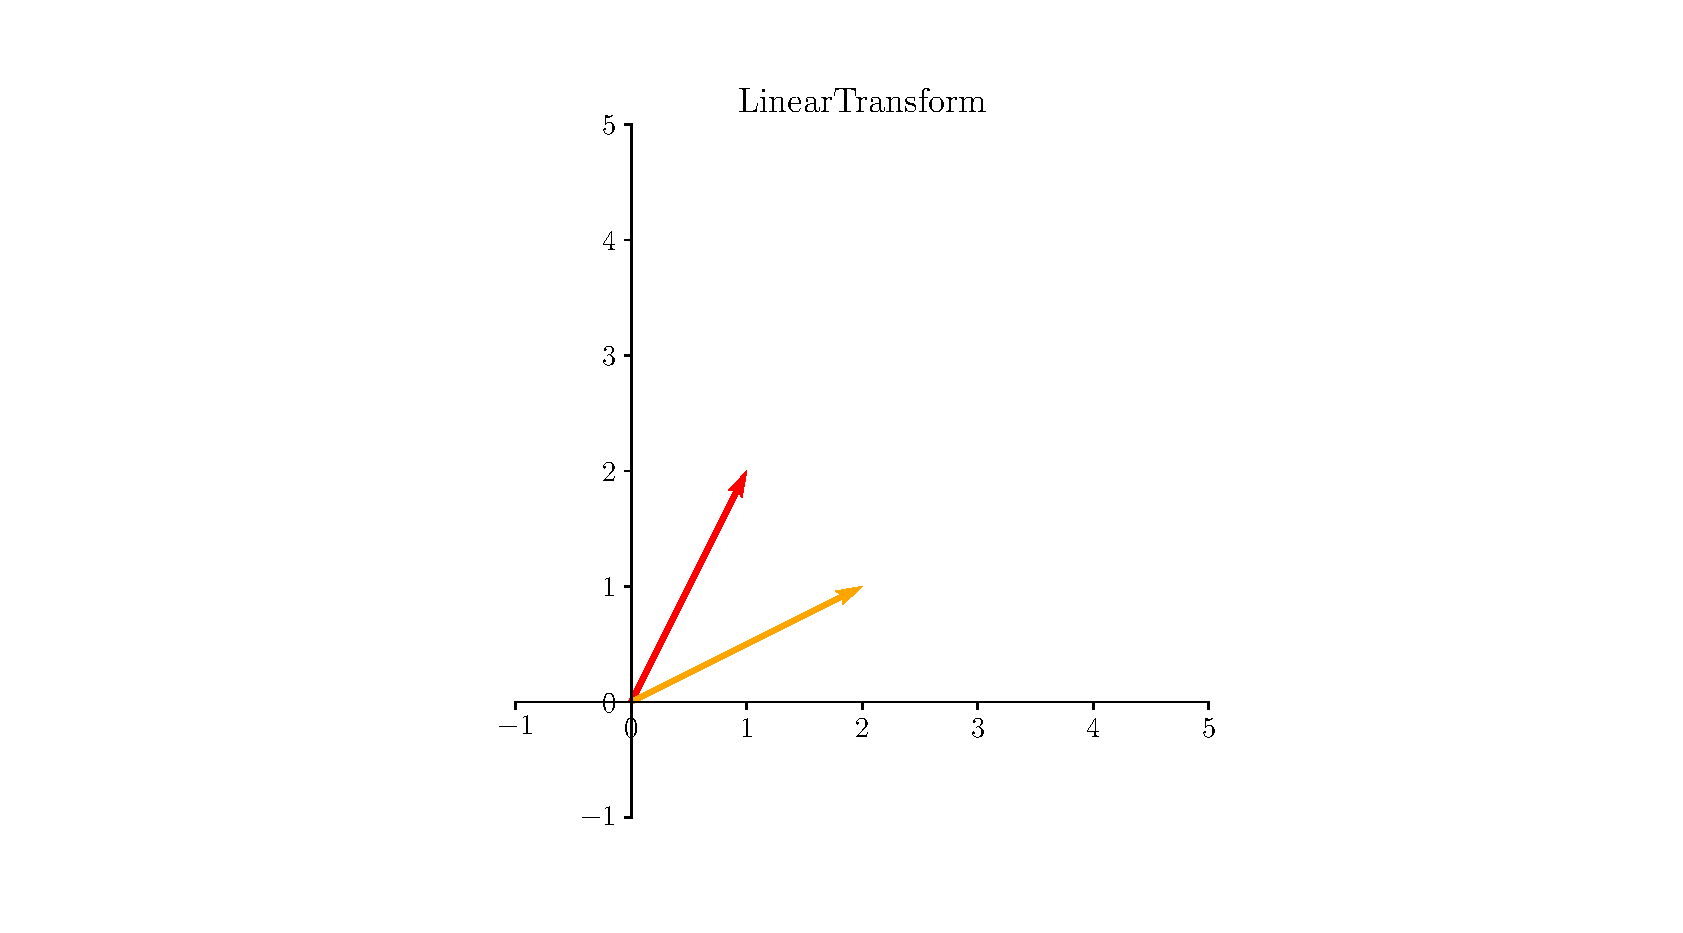
\includegraphics[width=0.7\linewidth]{figure/eps/LinearTransform.eps}
	\caption{线性变换}
	\label{fig:LinearTransform}
\end{figure}

我们平常所使用的坐标系是直角坐标系,表示向量使用标准基$\left\{ (1,0),(0,1) \right\}$,所谓的线性变换是指如果将坐标系进行一个变化,使得构成这个系的基由原来的$\left\{ (1,0),(0,1) \right\}$变化成$\left\{ (x_1,y_1),(x_2,y_2) \right\}$后所表示的向量在原坐标系中所表示的坐标。如图\ref{fig:LinearTransform}所示,如果我们的基由原来的$\left\{ (1,0),(0,1) \right\}$变化成$\left\{ (1,2),(2,1) \right\}$,那么变换前坐标$(4,5)$的线性组合是$(4,5)=4(1,0)+5(0,1)$,而变化基后的坐标则变为$(14,13)=4(1,2)+5(2,1)$,即空间内的每一点$(x,y)=x(1,0)+y(0,1)$都变化为$(x+2y,2x+y)=x(1,2)+y(2,1)$,设变化后的空间的每一个点在原坐标系的坐标表示为$(x',y')$;表示为线性方程组就是$$\left\{\begin{matrix} 
	1x+2y=x' \\  
	2x+1y=y'
  \end{matrix}\right. $$如果我们把这个式子进一步抽象,可以得到一个矩阵方程\begin{equation}
	\begin{pmatrix}  
	1 & 2 \\  
	2 & 1  
  \end{pmatrix} \begin{pmatrix}  
	x \\  
	y  
  \end{pmatrix} =\begin{pmatrix}  
	x' \\  
	y'  
  \end{pmatrix}
  \label{eq:MatrixIntro}
\end{equation}

\begin{example}
	\label{exam:scale}
	在平面直角坐标系中,向量$a=\overrightarrow{OP_1}=(3,2),b=\overrightarrow{OP_2}=(4,7)$;
	\begin{enumerate}
		\item 求$\triangle OP_1P_2$的面积;
		\item 若将$x$轴的每一个值扩大一倍,求标准基经过变换后的向量集合;
		\item 若将$y$轴的每一个值扩大一倍,求变换后的三角形面积$\triangle OP_1'P_2'$
	\end{enumerate}
	\tcblower
	\textcolor{purple}{\textbf{解}}:
	\begin{enumerate}
		\item 可使用割补法和叉积法,对于割补法,如图\ref{fig:source.gb}所示,则是将其填充为矩形,即$S=4\times 7-S_1-S_2-S_3$其中$S_1=4\times 7\div 2=14,S_2=(2+7)\times 1 \div 2=4.5,S_3=2\times 3 \div 2 =3$则$\triangle OP_1P_2$的结果为$S=28-14-18-3=6.5$,若使用叉积法,则有公式$$S=\frac{1}{2}\left| x_1y_2-x_2y_1 \right|=\frac{1}{2}=\left| 3\times 7-2\times 4 \right|=6.5$$
		\item $\left\{ (2,0),(0,1) \right\}$
		\item 若$y$轴扩大一倍,则该部分所有的面积都扩大一倍,所以$6.5\times 2=13$
	\end{enumerate}
\end{example}

\begin{figure}[htbp]    % 常规操作\begin{figure}开头说明插入图片
	% 后面跟着的[htbp]是图片在文档中放置的位置, 也称为浮动体的位置, 关于这个我们后面的文章会聊聊, 现在不管, 照写就是了
	\centering            % 前面说过, 图片放置在中间
	\subfloat[三角形$\triangle OP_1P_2$图]   % 第一张子图的下标(注意: 注释要写在[]中括号内)
	{
		\label{fig:source}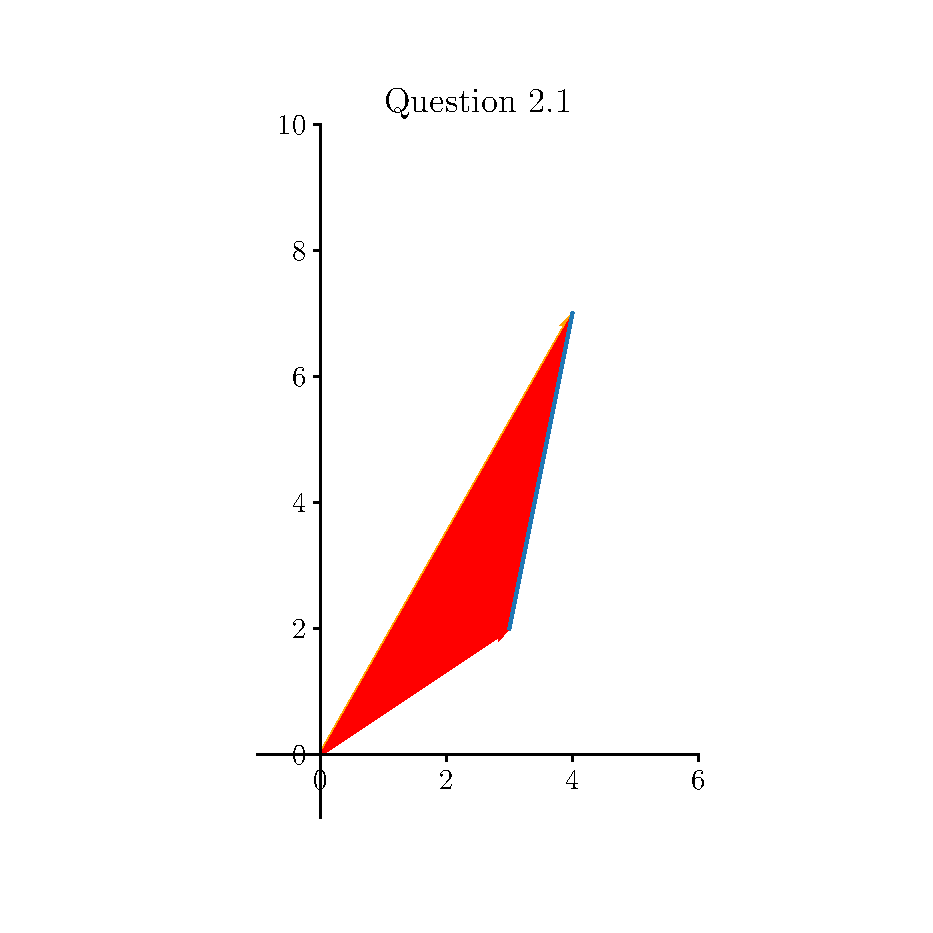
\includegraphics[width=0.5\textwidth]{eps/q21.eps}
		% \label{}命令为每个子图添加标签, 方便在正文中引用. 如果你不需要引用的话, 也可以不加这个命令, 写法在下面有: 
		% \label{}命令的{}内第一个{}中的内容fig:subfig1就是你插入的这张子图的标签, 注意每个标签都不能一样, 要用合适的编号去区分, 比如1, 2, 3......
		% \label{}命令中{}内\includegraphics[]{}就是真正插入图片的命令, []中的是图片的一些参数, {}就是图片的相对路径
		% width=0.4\textwidth 就是设置图片的大小, 这里设置的是文档宽度(\textwidth)的0.4倍, 在设置时注意不要超宽, 不然会报错, 大家多设置几个数尝试一下就能理解了
	}
	\subfloat[割补法]
	{
		\label{fig:source.gb}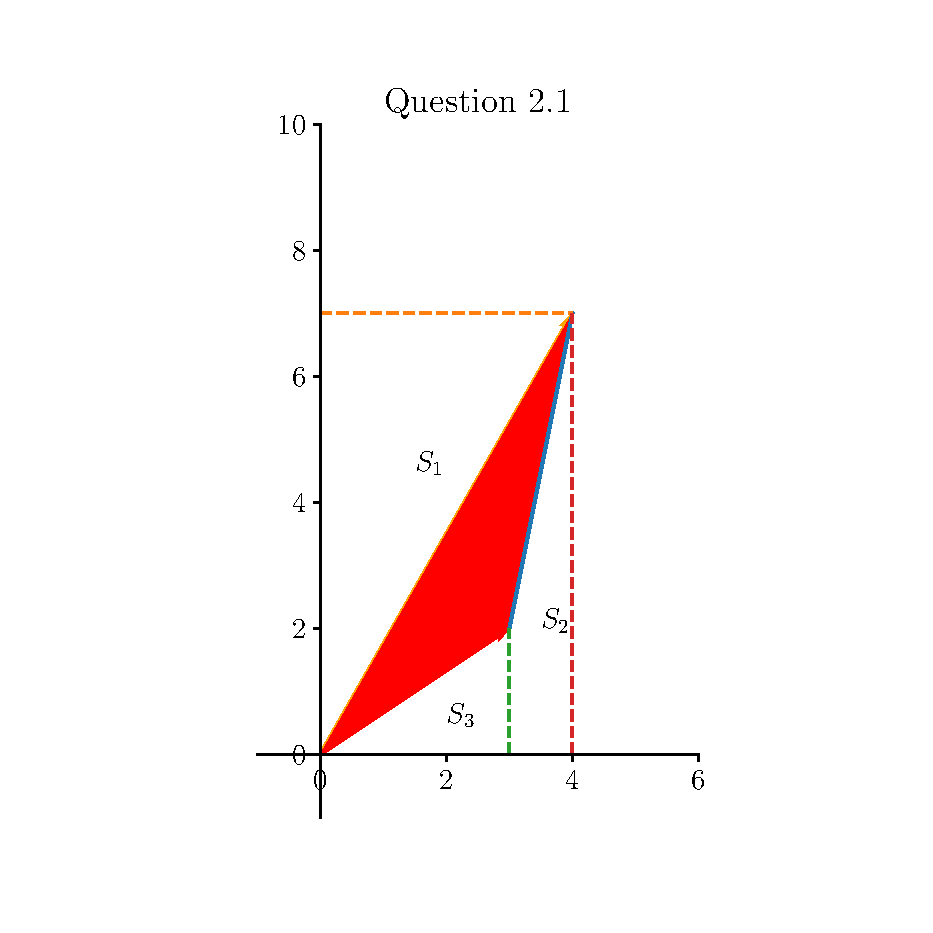
\includegraphics[width=0.5\textwidth]{eps/q21_gb.eps}
	}
	\caption{例题 2.1 图像}    % 整个图片的说明, 注释写在{}内
	\label{fig:pic.21}            % 整个图片的标签编号, 注意这里跟子图是一样的道理, 标签不能重复 
\end{figure}

为了方便表示,我们把公式\ref{eq:MatrixIntro}乘式中最左边的内容提取出来,称作变化矩阵,这个例子将是我们以后研究矩阵的一个特殊情况;为了方便描述,我们将该矩阵用$\mathbf{A}$表示
$$\mathbf{A}=\begin{pmatrix}  
	1 & 2 \\  
	2 & 1  
  \end{pmatrix}$$

若使用$\boldsymbol{x}$和$\boldsymbol{x'}$分别表示$(x,y)$和$(x',y')$的矩阵形式,那么公式\ref{eq:MatrixIntro}可表示为$$\boldsymbol{x'}=\mathbf{A}\boldsymbol{x}$$

接下来我们将矩阵$\mathbf{A}$中的第$i$行第$j$列元素表示为$\mathbf{A}_{i,j}$,例如$A_{1,2}=2$。

通过上面的描述,虽然我们并没有严格证明,但是我们也可以得知线性空间经过线性变换后,其结果仍然是线性空间。我们还是从二维平面出发来讲解矩阵的相关性质,于是我们有如下推论:

\begin{corollary}
	在二维平面内,矩阵$\mathbf{A}$表示其空间内的线性变换,设$x,y \in \mathbb{R}^2$且其矩阵表示分别为$\boldsymbol{x},\boldsymbol{y}$,则有如下推论:
	\begin{enumerate}
		\item $\mathbf{A}(\boldsymbol{x}+\boldsymbol{y})=\mathbf{A}\boldsymbol{x}+\mathbf{A}\boldsymbol{y}$
		\item 若$\lambda \in \mathbb{R}$则有$\lambda (\mathbf{A}\boldsymbol{x})=\mathbf{A}(c\boldsymbol{x})$
	\end{enumerate}
\end{corollary}

\begin{proof}
	\begin{enumerate}
		\item 设$x=(x_1,y_1),y=(x_2,y_2)$,则对于等式左侧$x+y=(x_1+x_2,y_1+y_2)$,其矩阵表示为$\begin{pmatrix}  
			x_1+y_1 \\  
			x_2+y_2  
		  \end{pmatrix} $,设$2\times 2$矩阵$\mathbf{A}$,令$$\mathbf{A}=\begin{pmatrix}  
			a & b \\  
			c & d  
		  \end{pmatrix} ,a,b,c,d \in \mathbb{R}$$那么类比矩阵方程\ref{eq:MatrixIntro},设结果向量为$(x',y')$我们可得矩阵式$$\begin{pmatrix}  
			a & b \\  
			c & d  
		  \end{pmatrix} \begin{pmatrix}  
			x_1+y_1 \\  
			x_2+y_2  
		  \end{pmatrix} $$的方程组式为$$\left\{\begin{matrix} 
			x'=a(x_1+y_1)+b(x_2+y_2) \\  
			y'=c(x_1+y_1)+d(x_2+y_2)
		  \end{matrix}\right. $$而根据标量加法分配法则,方程组可写成\begin{equation}\left\{\begin{matrix} 
			x'=ax_1+ay_1+bx_2+by_2 \\  
			y'=cx_1+cy_1+dx_2+dy_2
		  \end{matrix}\right. \label{eq:eqarray}\end{equation}同理右侧可表示为方程组式\ref{eq:eqarray},等式成立。$\square$
		\item 读者自证
	\end{enumerate}
\end{proof}

\subsection{矩阵表示线性方程组}

首先讲解什么是线性方程组,定义如下:

\begin{definition}{线性方程组}
	线性方程组是由多个线性方程组成的集合,通常表示为$$\begin{cases}
		a_{11}x_1 + a_{12}x_2 + \cdots + a_{1n}x_n = b_1 \\
		a_{21}x_1 + a_{22}x_2 + \cdots + a_{2n}x_n = b_2 \\
		\vdots \\
		a_{m1}x_1 + a_{m2}x_2 + \cdots + a_{mn}x_n = b_m
		\end{cases}$$
		其中,$ x_1, x_2, \ldots, x_n $ 是未知数,$ a_{ij} $ 是系数,$ b_i $ 是常数项。
\end{definition}

根据上面的矩阵式\ref{eq:MatrixIntro}所表示的二元一次方程组的几何意义,同样这里也可以看作是$n$维向量$x=(x_1,x_2,\\x_3,\cdots,x_n)$经过一个复杂的变化$\mathbf{A}$变为$b=(b_1,b_2,b_3,\cdots,b_n)$一样,所以同样我们可以将线性方程组的一般形式抽象成一个矩阵:$$\mathbf{A} \boldsymbol{x} = \boldsymbol{b}$$其中$$\mathbf{A} = \begin{pmatrix}
	a_{11} & a_{12} & \cdots & a_{1n} \\
	a_{21} & a_{22} & \cdots & a_{2n} \\
	\vdots & \vdots & \ddots & \vdots \\
	a_{m1} & a_{m2} & \cdots & a_{mn}
	\end{pmatrix},\boldsymbol{x}=\begin{pmatrix}
		x_1 \\
		x_2 \\
		\vdots \\
		x_n
		\end{pmatrix},\boldsymbol{b}=\begin{pmatrix}
			b_1 \\
			b_2 \\
			\vdots \\
			b_m
			\end{pmatrix}$$

\subsection{矩阵的定义}

我们已经对矩阵有了一个较为感性的认知,终于我们来到了系统讲解矩阵的这一部分,不过可能会让读者失望的是,矩阵的定义并非是你之前所认识的那样,是一个表示线性变换的符号;事实上,矩阵的真正定义其实就是一堆数字按照$m\times n$的方式排列而已,下面我们给出矩阵的定义。

\begin{definition}{矩阵的定义}
	矩阵是一个由圆括号\footnote{在一些教材中,会使用方形括号表示}包裹的按照矩形排列的$m\times n$的数表,一个 $m \times n$ 的矩阵 $ \mathbf{A} $ 可以表示为:
	$$\mathbf{A} = \begin{pmatrix}
		a_{11} & a_{12} & \cdots & a_{1n} \\
		a_{21} & a_{22} & \cdots & a_{2n} \\
		\vdots & \vdots & \ddots & \vdots \\
		a_{m1} & a_{m2} & \cdots & a_{mn}
		\end{pmatrix}$$其中:$ m $ 是行数,$ n $ 是列数。$ a_{ij} $ 表示矩阵中第 $ i $ 行第 $ j $ 列的元素。
\end{definition}

所有元素都是实数的矩阵叫作实矩阵,接下来我们将上面所讲到的$n\times 1$矩阵拓展到一般的矩阵计算。

\section{矩阵的运算法则}

\subsection{矩阵和}

\begin{definition}{$m\times n$矩阵的加法}
	若两个$m\times n$的同类型矩阵$\mathbf{A},\mathbf{B}$如果
	$$
	\mathbf{A} = \begin{pmatrix}
		a_{11} & a_{12} & \cdots & a_{1n} \\
		a_{21} & a_{22} & \cdots & a_{2n} \\
		\vdots & \vdots & \ddots & \vdots \\
		a_{m1} & a_{m2} & \cdots & a_{mn}
		\end{pmatrix},
		\mathbf{B} = \begin{pmatrix}
			b_{11} & b_{12} & \cdots & b_{1n} \\
			b_{21} & b_{22} & \cdots & b_{2n} \\
			\vdots & \vdots & \ddots & \vdots \\
			b_{m1} & b_{m2} & \cdots & b_{mn}
			\end{pmatrix},
	$$
	那么$$
	\mathbf{A}+\mathbf{B}=\begin{pmatrix}
		a_{11}+b_{11} & a_{12}+b_{12} & \cdots & a_{1n}+b_{1n} \\
		a_{21}+b_{21} & a_{22}+b_{22} & \cdots & a_{2n}+b_{2n} \\
		\vdots & \vdots & \ddots & \vdots \\
		a_{m1}+b_{m1} & a_{m2}+b_{m2} & \cdots & a_{mn}+b_{mn}
		\end{pmatrix}
	$$
\end{definition}

实际上,两个矩阵相加,就是把它们里面的所有元素依次相加并得到一个新的矩阵。与向量的加法相同的是,我们只定义了同类型的矩阵才能相加。

\begin{postulate}
	\label{pos:addOfMatrix}
	只有类型相同的矩阵才能互相相加。
\end{postulate}

那么也是和向量一样,它们满足交换律。

\begin{corollary}
	若$\mathbf{A},\mathbf{B},\mathbf{C}$均为$m\times n$的矩阵,它们满足交换律$\mathbf{A}+\mathbf{B}=\mathbf{B}+\mathbf{A}$和结合律$(\mathbf{A}+\mathbf{B})+\mathbf{C}=\mathbf{B}+(\mathbf{A}+\mathbf{C})$
\end{corollary}

请读者仿照向量的运算律,验证上述推论。

\subsection{0 矩阵}

根据公设\ref{pos:addOfMatrix},我们得知相同类型的矩阵的加法才有意义,所以我们定义在矩阵$\mathbf{A}+\mathbf{B}=\mathbf{A}$,那么$\mathbf{B}$就是 0 矩阵

\begin{definition}{0 矩阵}
	若$\mathbf{A},\mathbf{B}$均为$m\times n$的矩阵,且满足$\mathbf{A}+\mathbf{B}=\mathbf{A}$,那么$\mathbf{B}$为$m\times n$矩阵的单位元,显然,0 矩阵就是全是由 0 组成的矩阵,记作$\mathbf{O}$\footnote{不同于向量的记法,是以粗体形式出现的字母$\mathbf{O}$。},那么$$
	\mathbf{O}  = \begin{pmatrix}  
		0 & 0 & \cdots & 0 \\  
		0 & 0 & \cdots & 0 \\  
		\vdots & \vdots & \ddots & \vdots \\  
		0 & 0 & \cdots & 0  
	  \end{pmatrix} 
	$$
\end{definition}

\subsection{加法逆元}

类似于标量加法的$x,y\in \mathbb{C},x+y=0$与向量加法的$x,y\in \mathbb{F}^n,x+y=\boldsymbol{0}$,矩阵中同样表示若$\mathbf{A},\mathbf{B}$为同类型的矩阵,$\mathbf{A}+\mathbf{B}=\boldsymbol{O}$,$\mathbf{B}=-\mathbf{A}$表示$\mathbf{A}$的加法逆元。

\begin{definition}{加法逆元}
	对于矩阵$\mathbf{A}$,$\mathbf{A}$的加法逆元表示满足下面条件的矩阵$-\mathbf{A}$有$$\mathbf{A}+(-\mathbf{A})=\boldsymbol{O}$$换而言之当$$\mathbf{A}=\begin{pmatrix}  
		a_{11} & \cdots & a_{1n} \\  
		\vdots & \ddots & \vdots \\  
		a_{m1} & \cdots & a_{mn}  
	  \end{pmatrix} $$时,$$-\mathbf{A}=\begin{pmatrix}  
		-a_{11} & \cdots & -a_{1n} \\  
		\vdots & \ddots & \vdots \\  
		-a_{m1} & \cdots & -a_{mn}  
	  \end{pmatrix} $$
\end{definition}

\subsection{标量乘法}

\begin{definition}{矩阵的标量乘法}
	若标量$\lambda \in \mathbb{F}$,其对一个矩阵$\begin{pmatrix}  
		a_{11} & \cdots & a_{1n} \\  
		\vdots & \ddots & \vdots \\  
		a_{m1} & \cdots & a_{mn}  
	  \end{pmatrix} $的乘积满足以下的运算法则$$\lambda\begin{pmatrix}  
		a_{11} & \cdots & a_{1n} \\  
		\vdots & \ddots & \vdots \\  
		a_{m1} & \cdots & a_{mn}  
	  \end{pmatrix} =\begin{pmatrix}  
		\lambda a_{11} & \cdots & \lambda a_{1n} \\  
		\vdots & \ddots & \vdots \\  
		\lambda a_{m1} & \cdots & \lambda a_{mn}  
	  \end{pmatrix} $$
\end{definition}

同时,矩阵的标量乘法满足标量结合律。

\begin{corollary}
	若$a,b \in \mathbb{F}$,$\mathbf{A}$表示一个$m\times n$的矩阵,满足$(ab)\mathbf{A}=a(b\mathbf{A})$
\end{corollary}

\subsection{矩阵乘法}

这里讲一个特殊的乘法叫做矩阵乘法,矩阵乘法是线性代数中的一种基本运算,用于将两个矩阵相乘,得到一个新的矩阵。需要注意的是,我们在定义矩阵乘法的时候,只有左侧的矩阵行数等于右侧矩阵的列数,这个矩阵乘法才有意义,例如下面的矩阵乘法是有意义的。
\begin{enumerate}
	\item $\begin{pmatrix}  
		2 & 4 & 8\\    
	  \end{pmatrix} \begin{pmatrix}  
		1  \\  
		3  \\
		7
	  \end{pmatrix} $
	\item $\begin{pmatrix}  
		1 & 5 \\  
		8 & 1  
	  \end{pmatrix} \begin{pmatrix}  
		2 & 4 \\  
		3 & 7  
	  \end{pmatrix} $
\end{enumerate}

下面给出矩阵乘法的定义。

\begin{definition}{矩阵乘法的定义}
	\label{def:matrixMul}
	假设有两个矩阵 $ A $ 和 $ B $,其中 $ A $ 是一个 $ m \times n $ 的矩阵,$ B $ 是一个 $ n \times p $ 的矩阵,那么它们的乘积 $ C = A \times B $ 将是一个 $ m \times p $ 的矩阵。

矩阵乘法的计算规则如下:

对于矩阵 $ C $ 中的每一个元素 $ c_{ij} $,它是通过将矩阵 $ A $ 的第 $ i $ 行与矩阵 $ B $ 的第 $ j $ 列对应元素相乘后再相加得到的。具体公式为:$$c_{ij} = \sum_{k=1}^{n} a_{ik} \times b_{kj}$$
其中\begin{itemize}
	\item $ a_{ik} $ 是矩阵 $ A $ 的第 $ i $ 行第 $ k $ 列的元素,
	\item $ b_{kj} $ 是矩阵 $ B $ 的第 $ k $ 行第 $ j $ 列的元素。
\end{itemize}
\end{definition}

如定义所示,sigma符号还是如此的令人讨厌,读者不妨和笔者慢下来,在大脑内建立一个乘积的画面,下面我们给出矩阵乘法的直观操作。请注意,下面的内容请结合定义\ref{def:matrixMul}一起阅读,这样可以加深对矩阵加法的理解。

根据定义\ref{def:matrixMul},直观的矩阵乘应该以下面这样的结构进行相乘运算:$$\begin{pmatrix}  
	\xrightarrow[]{\qquad\qquad} \\  
	\xrightarrow[]{\qquad\qquad}  
  \end{pmatrix} \begin{pmatrix}  
	\myarrow & \myarrow\\
  \end{pmatrix}$$

最简单的如$\begin{pmatrix}  
	2 & 4 & 8\\    
  \end{pmatrix} \begin{pmatrix}  
	1  \\  
	3  \\
	7
  \end{pmatrix}$,乘法则为左矩阵从左往右,右矩阵从上到下,依次相乘的结果相加,我们可得
$$\begin{pmatrix}  
	\textcolor{red}{2} & \textcolor{blue}{4} & \textcolor{orange}{8} \\    
  \end{pmatrix} 
\begin{pmatrix}  
	\textcolor{red}{1}  \\  
	\textcolor{blue}{3}  \\
	\textcolor{orange}{7}
  \end{pmatrix} = (\textcolor{red}{1}\times \textcolor{red}{2}+\textcolor{blue}{3}\times \textcolor{blue}{4}+\textcolor{orange}{7}\times \textcolor{orange}{8})=(\textcolor{red}{2}+\textcolor{blue}{12}+\textcolor{orange}{56})=(70)\footnote{这里的70不是元组,也不是向量,而是$1\times 1$矩阵}
$$

再复杂一些,我们尝试$\begin{pmatrix}  
	1 & 5 \\  
	8 & 6  
  \end{pmatrix} \begin{pmatrix}  
	2 & 4 \\  
	3 & 7  
  \end{pmatrix}$,求矩阵就是重复按照上述操作填充表的过程,依照公式,
$c_{11}=a_{11}b_{11}+a_{12}b_{21}$
$$\begin{pmatrix}  
	\textcolor{red}{1} & \textcolor{blue}{5} \\  
	8 & 6  
  \end{pmatrix} \begin{pmatrix}  
	\textcolor{red}{2} & 4 \\  
	\textcolor{blue}{3} & 7  
  \end{pmatrix}=\begin{pmatrix}  
	\textcolor{red}{1}\times\textcolor{red}{2}+\textcolor{blue}{5}\times \textcolor{blue}{3}=17 & ? \\  
	? & ?  
\end{pmatrix} $$
以此类推,$c_{12}=a_{11}b_{12}+a_{12}b_{22}$
$$\begin{pmatrix}  
	\textcolor{red}{1} & \textcolor{blue}{5} \\  
	8 & 6  
  \end{pmatrix} \begin{pmatrix}  
	2 & \textcolor{red}{4} \\  
	3 & \textcolor{blue}{7}  
  \end{pmatrix}=\begin{pmatrix}  
	17&\textcolor{red}{1}\times \textcolor{red}{4} +\textcolor{blue}{5}\times \textcolor{blue}{7} =39 \\  
	? & ?  
\end{pmatrix} $$

$c_{21}=a_{21}b_{11}+a_{22}b_{21}$

$$\begin{pmatrix}  
	1 & 5 \\  
	\textcolor{red}{8} & \textcolor{blue}{6}  
  \end{pmatrix} \begin{pmatrix}  
	\textcolor{red}{2} & {4} \\  
	\textcolor{blue}{3} & {7}  
  \end{pmatrix}=\begin{pmatrix}  
	17 & 39 \\  
	\textcolor{red}{8}\times \textcolor{red}{2}+\textcolor{blue}{6} \times\textcolor{blue}{3}=34 & ?  
\end{pmatrix} $$

$c_{22}=a_{21}b_{12}+a_{22}b_{22}$

$$\begin{pmatrix}  
	1 & 5 \\  
	\textcolor{red}{8} & \textcolor{blue}{6}  
  \end{pmatrix} \begin{pmatrix}  
	{2} & \textcolor{red}{4} \\  
	{3} & \textcolor{blue}{7}  
  \end{pmatrix}=\begin{pmatrix}  
	17 & 39 \\  
	34 & \textcolor{red}{8}\times \textcolor{red}{4}+\textcolor{blue}{6}\times \textcolor{blue}{7}=74
\end{pmatrix} $$

至此,我们填充了整个矩阵表,所以$\begin{pmatrix}  
	1 & 5 \\  
	8 & 6  
  \end{pmatrix} \begin{pmatrix}  
	2 & 4 \\  
	3 & 7  
  \end{pmatrix}=\begin{pmatrix}  
	17 & 39 \\  
	34 & 74  
  \end{pmatrix} $

\begin{example}
	求下列矩阵的乘积:
	\begin{enumerate}
		\item $\begin{pmatrix}  
			1 & 4 & -1 \\  
			-2 & 6 & 5  
		  \end{pmatrix} \begin{pmatrix}  
			0 & 2 & 5 \\  
			-1 & 1 & 7 \\
			3 & 2 & -3
		  \end{pmatrix}$
		\item $\begin{pmatrix}  
			1 & 1 & -4 \\  
			5 & -1 & 4 \\
			-1 & 9 & 1
		  \end{pmatrix}\begin{pmatrix}  
			9 \\
			8 \\
			1
		  \end{pmatrix}$
		\item $\begin{pmatrix}  
			a & b \\  
			c & d  
		  \end{pmatrix} \begin{pmatrix}  
			e & f \\  
			g & h  
		  \end{pmatrix} $
		\item $\begin{pmatrix}  
			e & f \\  
			g & h  
		  \end{pmatrix} \begin{pmatrix}  
			a & b \\  
			c & d  
		  \end{pmatrix} $
		\item 矩阵乘法是否满足交换律?
	\end{enumerate}
	\tcblower
	\textcolor{purple}{\textbf{解}}:
	\begin{enumerate}
		\item $\begin{pmatrix}  
			-7 & 4 & 36 \\  
			9 & 12 & 17 \\  
		  \end{pmatrix} $
		\item $\begin{pmatrix}  
			21 \\  
			41 \\ 
			64 
		  \end{pmatrix} $
		\item $\begin{pmatrix}  
			bg+ae & af+bh \\  
			cd+gh & cf+dh  
		  \end{pmatrix} $
		\item $\begin{pmatrix}  
			cf+ae & df+be \\  
			ag+ch & bg+dh  
		  \end{pmatrix} $
		\item 否
	\end{enumerate}
\end{example}

\subsection{平面上的线性变换}

欲要了解矩阵的作用,我们先来了解一下线性变换。

平面上的线性变换是指通过一个矩阵将平面上的每一个点(向量)映射到另一个点的变换。这种变换满足线性性质,即保持向量加法和标量乘法。

在平面直角坐标系内,常见的线性变换包括:
\begin{enumerate}
	\item 缩放:沿坐标轴方向拉伸或压缩,例如例题\ref{exam:scale}的第2,3小问;
	\item 旋转:坐标轴绕原点旋转一定角度$\theta$;
	\item 剪切:使图形沿某一方向倾斜,例如图\ref{fig:pic.21};
	\item 反射:关于某条直线或点的对称变换。
\end{enumerate}

由此,我们可以得到在$\mathbb{R}^2$线性变换的性质:

\begin{itemize}
	\item 保持原点不变;
	\item 保持直线性:直线变换后仍为直线。
\end{itemize}

而矩阵则表示了线性变换的过程,矩阵与矩阵的乘积表示线性变换后的过程,在这里我们介绍一个术语叫做左乘,矩阵的乘法表示一般从右往左写,例如:如果我们将正交的直角坐标系中的每一个向量都顺时针旋转$\alpha$,那么一个向量$a=(x,y)$经过变化后的坐标$(x',y')$满足下面这一个式子:
$$
\left\{\begin{matrix} 
	x'=\cos \alpha \cdot x-\sin \alpha \cdot y \\  
	y'=\sin \alpha \cdot x+\cos \alpha \cdot y
  \end{matrix}\right. 
$$
接下来我们将这个方程组抽象为矩阵,可得
$$
\begin{pmatrix}  
	x' \\  
	y'  
  \end{pmatrix} =\begin{pmatrix}  
	\cos \alpha & -\sin \alpha  \\  
	\sin \alpha & \cos \alpha   
  \end{pmatrix} \begin{pmatrix}  
	x \\  
	y
  \end{pmatrix} 
$$
提取矩阵并给其一个符号
$$
\mathbf{A}=\begin{pmatrix}  
	\cos \alpha & -\sin \alpha  \\  
	\sin \alpha & \cos \alpha   
  \end{pmatrix} 
$$
仔细观察矩阵$\mathbf{A}$第一列的两个数按序写成2元组,即为$(\cos \alpha,\sin \alpha)$,如果读者观察仔细的话,正是标准基其中的一个$(1,0)$经过该变换后的坐标,而第二列的$(-\sin \alpha,\cos \alpha)$是标准基另一个$(0,1)$变化后的坐标,而该矩阵乘积所得的矩阵,正是变化后在原坐标系中的向量表示。

那如果我们在旋转的基础上继续旋转$\beta$弧度,我们直接可以得到矩阵$\mathbf{C}=\begin{pmatrix}  
	\cos (\alpha+\beta) & -\sin (\alpha+\beta)  \\  
	\sin (\alpha+\beta) & \cos (\alpha+\beta) 
\end{pmatrix} $,如果表示成两个矩阵相乘,则是矩阵$\mathbf{A}$左乘一个矩阵$\mathbf{B}$,该矩阵$\mathbf{B}$即为只旋转$\beta$弧度的矩阵表示,则
$$
\mathbf{B}=\begin{pmatrix}  
	\cos \beta & -\sin \beta  \\  
	\sin \beta & \cos \beta   
  \end{pmatrix} 
$$
写完整些是这样的
$$
\begin{pmatrix}  
	\cos (\alpha+\beta) & -\sin (\alpha+\beta)  \\  
	\sin (\alpha+\beta) & \cos (\alpha+\beta) 
\end{pmatrix}=\begin{pmatrix}  
	\cos \beta & -\sin \beta  \\  
	\sin \beta & \cos \beta   
  \end{pmatrix} \begin{pmatrix}  
	\cos \alpha & -\sin \alpha  \\  
	\sin \alpha & \cos \alpha   
  \end{pmatrix} 
$$
请读者按照矩阵的乘法验证该等式成立。

\section{线性映射}

\subsection{从平面走向更高维度}

线性代数研究的不只是平面,更是更高维度的内容,如果我们把目光从平面$\mathbb{R}^2$与$\mathbb{R}^3$上移到$\mathbb{F}^n$,那么我们现在把``线性变换''这个词改一个说法,改成``线性映射''来表示一种函数。

\subsection{线性空间中的线性映射}

如果读者忘记了什么是线性空间,请回到章节\ref{subsec:linearSpace}回顾一下它们的基本性质,在线性空间中,线性映射表示的是一个线性空间$V$的元素到另一个线性空间的元素$W$,即$T: V\rightarrow W$

\begin{definition}{线性映射}
	若$V,W$均为线性空间,$y\in W,x\in V$,则函数$y=T(x)$表示线性映射当且仅当满足下面的性质:
	\begin{enumerate}
		\item 加性(additivity):对所有$u,v\in V$都有$T(u+v)=T(u)+T(v)$;
		\item 齐性(homogeneity):对所有$\lambda \in \mathbb{F}$和$v\in V$都有$T(\lambda v)=\lambda T(v)$
	\end{enumerate}
	通常满足从$V$到$W$的所有线性映射所构成的集合记为$\mathcal{L}(V,W)$,例如上面的函数$T\in\mathcal{L}(V,W)$
\end{definition}

\begin{ascolorbox1}{思考}
	分别验证在平面上的旋转,剪切,缩放是一种线性映射。
\end{ascolorbox1}

对于旋转线性映射,设$V$是映射前的空间,映射前向量$v=(x,y),v\in V$经过绕远点旋转$\alpha$后其空间变为$W$,设$w=(x',y'),w\in W$为映射后的向量,那么它们满足$$
\begin{pmatrix}  
	x' \\  
	y'  
  \end{pmatrix} =\begin{pmatrix}  
	\cos \alpha & -\sin \alpha  \\  
	\sin \alpha & \cos \alpha   
  \end{pmatrix} \begin{pmatrix}  
	x \\  
	y
  \end{pmatrix} 
$$
首先他们满足加性,若有向量$v_1=(x_1,y_1)$,旋转后则变为$w_1=(x_1',x_2')$满足
$$
\begin{pmatrix}  
	x_1' \\  
	y_1'  
  \end{pmatrix} =\begin{pmatrix}  
	\cos \alpha & -\sin \alpha  \\  
	\sin \alpha & \cos \alpha   
  \end{pmatrix} \begin{pmatrix}  
	x_1 \\  
	y_1
  \end{pmatrix} 
$$
则一定满足
$$
\begin{pmatrix}  
	x'+x_1' \\  
	y'+y_1'  
  \end{pmatrix} =\begin{pmatrix}  
	\cos \alpha & -\sin \alpha  \\  
	\sin \alpha & \cos \alpha   
  \end{pmatrix} \begin{pmatrix}  
	x+x_1 \\  
	y+y_1
  \end{pmatrix} 
$$
其次他们满足齐性,设$\lambda \in \mathbb{F}$,则有
$$
\begin{pmatrix}  
	\lambda x' \\  
	\lambda y'  
  \end{pmatrix} =\begin{pmatrix}  
	\cos \alpha & -\sin \alpha  \\  
	\sin \alpha & \cos \alpha   
  \end{pmatrix} \begin{pmatrix}  
	\lambda x \\  
	\lambda y
  \end{pmatrix} 
$$
所以旋转在平面上是一种线性映射,限于篇幅,请读者自行验证剪切与放缩。

\subsection{零空间}

我们将线性映射从$V$到$W$中,将原来空间中的某个映射为$\boldsymbol{0}$的子空间叫做零空间,下面给出其定义:

\begin{definition}{零空间(null space)}
	对于映射$T:V\rightarrow W$,$T$的零空间是在$V$中经过$T$映射为$\boldsymbol{0}$ 向量的子空间,记为$\text{null}T$\footnote{有些书本会使用核空间,并记作$Ker~T$},则$$\text{null}T=\left\{ v\in V: T(v)\footnote{对于线性映射$T$,一些书本会将其简写为$Tv$}=0 \right\}$$
\end{definition}

同样用$\mathbb{R}^2$的例子,存在一个映射$T: \mathbb{R}^2\rightarrow \mathbb{R}^2$,$T\in \mathcal{L}(\mathbb{R}^2,\mathbb{R}^2)$,若表示这是一个将平面上的所有点压缩为一条线的一个映射,设该法则将$v\in \mathbb{R}^2,v=(x,y)$映射为$w\in \mathbb{R}^2,w=(x,0)$,记为$T(v)=w$或$T((x,y))=(x,0)$,那么零空间$\text{null}T$则为:
$$
\text{null}T=\left\{ (0,t)\mid t\in \mathbb{R} \right\}
$$
\begin{ascolorbox1}{思考}
	上面的$\text{dim}~\text{null}T$的值是多少?
\end{ascolorbox1}

由于$\text{null}T$只需要一个基$\left\{ (0,1) \right\}$,使得任意一个$v\in \text{null}T$存在$\alpha\in \mathbb{R}$满足$v=\alpha (0,1)$表示,所以$\text{dim}~\text{null}T=1$,即使它放在了$\mathbb{R}^2$中。

\begin{example}
	若$\varphi \in \mathcal{L}(\mathbb{C}^3,\mathbb{C}),v_1\in \mathbb{C}^3,v_2\in \mathbb{C}$,定义线性映射$\varphi(v_1)=v_2$,其中$v_1=(x_1,x_2,x_3)$,$v_2=x_1+2x_2+3x_3$则$\varphi((x_1,x_2,x_3))=x_1+2x_2+3x_3$\footnote{如果以后没有特殊说明,在线性映射中的每个未知数前后相通},求$\text{null}\varphi$的一个基集合与$\text{null}\varphi$的维数。
	\tcblower
	\textcolor{purple}{\textbf{解}}:$\text{null}\varphi=\left\{ (a,b,c)\mid a+2b+3c=0 \right\}$令$a=0$则$b=3,c=-2$,若令$b=0$则$a=-3,c=1$,若令$c=0$则$a=-2,b=1$而向量$c$可由$a,b$的线性组合得到,所以3者向量线性相关,故去除一个向量后二者向量线性无关,则$\text{null}\varphi$的一个基为$\left\{ (0,3,-2),(-3,0,1) \right\}$\footnote{后面我们会讲解求线性方程组并使用更加正确的方式求基},根据基的元素个数,我们可以推断$\text{dim}~\text{null}\varphi =2$。
\end{example}

\subsection{值域空间}

作为一个函数有个映射法则$T$,那么我们给经过$T$映射后的空间取个名字叫做值域空间。

\begin{definition}{值域空间(range space)}
	对于映射$T:V\rightarrow W$,$T$的值域空间是在$V$中经过$T$法则映射为$W$的所有元素的集合,记作$\text{range}T$\footnote{有些书本会使用像空间,并记作$Im~T$},则
	$$
	\text{range}T=\left\{ T(v)\mid v\in V \right\}
	$$
\end{definition}

用之前一个$\mathbb{R}^2$的例子,存在一个映射$T: \mathbb{R}^2\rightarrow \mathbb{R}^2$,$T\in \mathcal{L}(\mathbb{R}^2,\mathbb{R}^2)$,若表示这是一个将平面上的所有点压缩为一条线的一个映射,设该法则将$v\in \mathbb{R}^2,v=(x,y)$映射为$w\in \mathbb{R}^2,w=(x,0)$,记为$T(v)=w$或$T((x,y))=(x,0)$,那么值域空间$\text{range}T$则为:
$$
\text{range}T=\left\{ (t,0)\mid t\in \mathbb{R} \right\}
$$
很显然,此处的$\text{dim}~\text{range}T=1$。
\begin{example}
	%\label{exam:rangeT}
	若$\varphi \in \mathcal{L}(\mathbb{C}^3,\mathbb{C}),v_1\in \mathbb{C}^3,v_2\in \mathbb{C}$,定义线性映射$\varphi(v_1)=v_2$,其中$v_1=(x_1,x_2,x_3)$,$v_2=x_1+2x_2+3x_3$则$\varphi((x_1,x_2,x_3))=x_1+2x_2+3x_3$,求$\text{range}\varphi$的一个基集合与$\text{range}\varphi$的维数。
	\tcblower
	\textcolor{purple}{\textbf{解}}:$\text{range}\varphi=\mathbb{C}$那么$\text{null}\varphi$的一个基为$\left\{ 1 \right\}$,也就是说$\mathbb{C}$上的任意一个元素都可以用$\alpha 1,\alpha\in \mathbb{C}$的线性组合表示,所以$\text{dim}~\text{range}\varphi =1$。
\end{example}

\subsection{线性映射基本定理}

下面是一个非常重要的一个定理。

\begin{theorem}{线性映射基本定理}
	$V,W$是有限维线性空间,法则$T\in\mathcal{L}(V,W),T:V\rightarrow W$使得下述成立:$$\text{dim}V=\text{dim}~\text{null}T+\text{dim}~\text{range}T$$
\end{theorem}

\begin{proof}
	设$A=\left\{ v_1,v_2,v_3,\cdots,v_m \right\}$是$\text{null}T$,则$\text{dim}~\text{null}T=m$且集合$\left\{ v_1,v_2,v_3,\cdots,v_m \right\}$线性无关,那么$V$的基一定包含集合$B$,但是$V$的基的元素个数一定大于$B$元素的个数,可设$\left\{ v_1,v_2,v_3,\cdots,v_m,u_1,u_2,\cdots,u_m \right\}$是$V$的基,则$\text{dim}V=m+n$;我们只需要证明$\text{dim}~\text{range}T=n$。

	对于每一个$v\in V$都可以使用$\left\{ v_1,v_2,v_3,\cdots,v_m,u_1,u_2,\cdots,u_m \right\}$的线性组合表示,即$$v=a_1v_1+a_2v_2+a_3v_3+\cdots+a_mv_m+b_1u_1+b_2u_2+\cdots+b_mu_m,a_i\in \mathbb{F},i\in \mathbb{N}^+\footnote{$\mathbb{N}^+$代表正整数}$$对等式两边的所有向量进行$T$法则映射,则一部分属于$\text{null}T$的基$A$将会被映射为$\boldsymbol{0}$,即$$T(v)=\boldsymbol{0}+\boldsymbol{0}+\boldsymbol{0}+\cdots+\boldsymbol{0}+b_1T(u_1)+b_2T(u_2)+\cdots+b_mT(u_m)$$所以我们可以得到$A_{T}=\left\{ T(u_1),T(u_2),T(u_3),\cdots,T(u_m) \right\}$张成$\text{range}T$,即$\text{Span}(A_{T})=\text{range}T$。

	下面继续证明$A_{T}$线性无关,设$\boldsymbol{0}$可以由$A_{T}$的线性组合得到,即$$c_1T(u_1)+c_2T(u_2)+c_3T(u_3)+\cdots+c_nT(u_n)=\boldsymbol{0}$$那么根据线性映射的标量乘法的性质$$T(c_1u_1+c_2u_2+c_3u_3+\cdots+c_mu_m)=\boldsymbol{0}$$设$u=c_1u_1+c_2u_2+c_3u_3+\cdots+c_mu_m$则有$u\in \text{null}T$,而$\text{Span}(A)=\text{null}T$且$A$线性无关,那么当且仅当$c_1=c_2=c_3=\cdots=c_m=0$时,可由$A$的线性组合表示$u$,此时仅可表示$\boldsymbol{0}$向量,所以$A_{T}$线性无关,故$\text{range}T$的基为$\left\{ u_1,u_2,\cdots,u_m \right\}$,所以\begin{equation*}
		\text{dim}V=\text{dim}~\text{null}T+\text{dim}~\text{range}T \teoe
	\end{equation*}
\end{proof}

拿之前的例子我们验证该定理,例如例题2.4所表示的那样,$\text{dim}\mathbb{R}^3=3$,$\text{null}\varphi=\left\{ (a,b,c)\mid a+2b+3c=0 \right\}$则$\text{dim}~\text{null}\varphi=2$,同时$\text{dim}~\text{range}\varphi =1$满足题设条件。

其实这个定理也说明了线性映射后只会丢失信息而不会增加信息,线性映射后的空间维度只会减少不会增加,即使你是$\mathcal{L}(\mathbb{R}^2,\mathbb{R}^3)$看似升高维度,实际上这种映射在三维空间中还是一个平面,只不过这个平面只能在三维空间中表示。所以它们只需要两个线性无关的向量的线性组合就可以表示映射后空间内所有的向量。

\section{矩阵表示线性映射}

\subsection{线性映射的运算法则}

线性映射也有加法和标量乘法,它们定义如下:

\begin{definition}{线性映射的加法与标量乘法}
	若$S,T\in \mathcal{L}(V,W)$,$\alpha\in \mathbb{F}$则$S+T$是一个从$V$到$W$的线性映射,若$v\in V$,它们满足$$(S+T)(v)=S(v)+T(v)$$
	标量积$\alpha T$满足$$(\alpha T)(v)=\alpha(T(v))$$
\end{definition}

此外,线性映射也有相乘操作,它们如同矩阵一样,从右往左相乘,表示先进行右边的线性映射,再进行左边的线性映射。

\begin{definition}{线性映射的乘法}
	若$S,T\in \mathcal{L}(V,W)$,则$ST$是一个从$V$到$W$的线性映射,若$v\in V$,它们满足$$(ST)(v)=S(T(v))\footnote{从右往左,一定是先进行$T$再进行$S$}$$
\end{definition}

\subsection{矩阵描述线性映射}

根据线性映射的基本定理,我们知道经过线性映射后维度不会升高,若$\left\{ v_1,v_2,v_3,\cdots,v_n \right\}$为$V$的一个基,对于每一个经过线性映射$T\in \mathcal{L}(V,W)$的基为$W_t=\left\{ Tv_1,Tv_2,Tv_3,\cdots,Tv_n \right\}$必然有$\text{range}T=\text{Span}(W_t)$,接下来我们使用矩阵记录$V$上的基的每一项经过映射后的$T(v_i)$,都可以由$W$上的基的线性组合表示。

这么说可能有些抽象且复杂,我们给出定义并从定义入手:

\begin{definition}{线性映射的矩阵表示}
	设$T\in\mathcal{L}(V,W)$,$\left\{ v_1,v_2,v_3,\cdots,v_n \right\}$是线性空间$V$的基,$\mathcal{M}(T)$为$m\times n$的矩阵,其元素的第$i$行第$j$列表示为$a_{ij}$,那么根据这些基的线性映射的矩阵表示中的元素$a_{ij}$满足
	$$T(v_k)=a_{1k}w_1+a_{2k}w_2+a_{3k}w_3+\cdots+a_{mk}w_m$$
\end{definition}

或许读者会感觉这个定义更加抽象了,我们还是不妨使用老朋友$\mathbb{R}^2$和$\mathbb{R}^3$来描述。

\begin{example}
	设$T\in \mathcal{L}(\mathbb{R}^2,\mathbb{R}^3)$若向量$a=(x,y)$经过变换后的向量为$b=(x+3y,2x+5y,7x+9y)$那么$T(a)=b,T((x,y))=(x+3y,2x+5y,7x+9y)$,求关于$\mathbb{R}^2$与$\mathbb{R}^3$上的标准基$\left\{ (1,0),(0,1) \right\}$和$\left\{ (1,0,0),(0,1,0),(0,0,1) \right\}$线性映射的矩阵表示。\footnote{本题参见Linear Algebra Done Right的3.33}
	\tcblower
	\textcolor{purple}{\textbf{解}}:$T((1,0))=(1,2,7)$那么$\mathbb{R}^3$的标准基$w_1=(1,0,0),w_2=(0,1,0),w_3=(0,0,1)$可表示为$$v_1=(1,0),T(v_1)=(1,2,7)=1w_1+2w_2+7w_3$$所以$(1,2,7)$依次为矩阵第一列的元素$a_{11},a_{21},a_{31}$,而$T((0,1))=(3,5,9)$,那么$$v_2=(0,1),T(v_2)=(3,5,9)=3w_1+5w_2+9w_3$$所以$(3,5,9)$依次为矩阵第二列的元素$a_{12},a_{22},a_{32}$,所以关于标准基的线性映射矩阵表示为$$\begin{pmatrix}  
		1 & 3 \\  
		2 & 5 \\
		7 & 9 
	  \end{pmatrix} $$
\end{example}

前文我们说过线性映射也有自己的运算法则,然后矩阵也有自己的运算法则,那么两者之间是否存在关系,或者说这两者可以是统一的呢?其实答案相信对在座的学霸们来说已经能够看到这两者的关系了。

线性映射的加法可以描述为法则$S,T$将向量$v$经过这两个法则映射后的和,反应在矩阵上便有如下的推论(我们假设$S,T,S+T$都使用同样的基):

\begin{corollary}
	若$S,T\in \mathcal{L}(V,W),\alpha\in\mathbb{F}$,则$\mathcal{M}(S+T)=\mathcal{M}(S)+\mathcal{M}(T),\alpha\mathcal{M}(T)=\mathcal{M}(\alpha T)$。
\end{corollary}

同样的道理,线性映射的乘法同样可以抽象为矩阵的乘法,需要注意的是,它们都不满足交换律,表示从右往左,先后映射的内容。

\begin{corollary}
	若$T\in \mathcal{L}(U,V),S\in \mathcal{L}(V,W)$则$\mathcal{M}(ST)=\mathcal{M}(S)\mathcal{M}(T)$。
\end{corollary}

\section{章节练习}

\subsection{A组}

\begin{reidai}
	计算矩阵$\mathbf{A}=\begin{pmatrix}  
		3 & -1 & 5 \\  
		\sqrt{2} & 4 & 0 \\  
		-2 & -7 & 6  
	  \end{pmatrix} $与$\mathbf{B}=\begin{pmatrix}  
		3 & 2 & \sqrt{7} \\  
		4 & -2 & 1 \\  
		-5 & 0 & 6  
	  \end{pmatrix} $的和。
\end{reidai}

\begin{reidai}
	计算矩阵$\mathbf{A}=\begin{pmatrix}  
		1 & 3+\mathrm{i} & \sqrt{5}  \\  
		2-\mathrm{i} & 3 & -4 
	  \end{pmatrix} $与$\mathbf{B}=\begin{pmatrix}  
		-1 & \mathrm{i} & \sqrt{2} & 4  \\  
		9 & 3 & -4 & 3 \\
		2-\mathrm{i} & 4 & 8 & 1
	  \end{pmatrix} $的乘积。
\end{reidai}

\begin{reidai}
	若$T\in \mathcal{L}(\mathbb{R}^3,\mathbb{R}^2)$,有$$T((x,y,z))=(a+x+y,bxyz)$$求$b,c$的值。
\end{reidai}

\begin{reidai}
	根据线性映射的加法和标量乘法,试证明$\mathcal{L}(V,W)$是线性空间。
\end{reidai}

\begin{reidai}
	三体文明有一个工具叫做二向箔,这个工具可以将空间二维化,设该变化为简单的线性映射$T:V\rightarrow W$,$T\in \mathcal{L}(V,M)$满足$$T((x,y,z))=(x,y)$$求$\text{range}T$和$\text{null}T$。
\end{reidai}

\begin{reidai}
	平面上有三点$A(3,2),B(-1,4),C(2,0)$,请使用叉积法求$S_{\triangle ABC}$。
\end{reidai}

\begin{reidai}
	三维空间$\mathbb{R}^3$中任意一点$(x,y,z)$,若将$\mathbb{R}^3$的标准基均向直线方向$x=y=z$旋转$\displaystyle \frac{\pi}{3}$,请使用关于$(x,y,z)$的矩阵式表示$(x',y',z')$
\end{reidai}

\begin{reidai}
	举例线性映射$T$使得$\text{dim}~\text{range}T=2,\text{dim}~\text{null}T=3$
\end{reidai}

\subsection{B组}

\begin{reidai}
	线性方程组常数项为0
	$$\left\{\begin{matrix} 
		a_{11}x_1+a_{12}x_2+a_{13}x_3+\cdots+a_{1n}x_n=0 \\  
		a_{21}x_1+a_{22}x_2+a_{23}x_3+\cdots+a_{2n}x_n=0 \\
		\cdots \\
		a_{m1}x_1+a_{m2}x_2+a_{m3}x_3+\cdots+a_{mn}x_n=0
	\end{matrix}\right. $$可视为线性映射$$T(x_1,x_2,\cdots,x_n)=\left( \sum_{i=1}^{n}a_{1i}x_i,\sum_{i=1}^{n}a_{2i}x_i,\cdots,\sum_{i=1}^{n}a_{mi}x_i \right)$$
	除$x_1=x_2=x_3=\cdots=x_n=0$外,$\text{dim}~\text{null}T$需要满足条件才有其他解?
\end{reidai}

\begin{reidai}
	若$S\in\mathcal{L}(V,W),T\in\mathcal{L}(U,V)$求证$$\text{dim}~\text{null}ST\le \text{dim}~\text{null}S+\text{dim}~\text{null}T$$
\end{reidai}

\begin{reidai}
	请不要看笔者的证明过程,自己复盘一遍线性映射的基本定理,并尝试自己写证明过程。
\end{reidai}



\chapterimage{chapters/3.jpg}
\chapter{内积空间}
\begin{center}
	% \textcolor[RGB]{255, 0, 0}{\faHeart}所以生命啊,它苦涩如歌.\textcolor[RGB]{255, 0, 0}{\faHeart}
	「花有重开日,人无再少年」
\end{center}
\rightline{——《续侄溥赏酴醾劝酒二首·其一》}
\vspace{-5pt}
\begin{center}
	\pgfornament[width=0.36\linewidth,color=lsp]{88}
\end{center}

\section{内积}

\subsection{向量的点积与长度表示}

本章请读者自行考虑是否阅读,如果读者对线性代数要求不是那么高,可以跳过该章节,本章较有难度,但是看下去会很有意思。

在高中的学习生涯中,我们总是把二维空间$\mathbb{R}^2$与三维空间$\mathbb{R}^3$中的向量具体化为一个有向箭头。通常我们求两点之间的坐标距离会使用勾股定理,在前面的学习中,定义\ref{def:lengthOfVec}就是使用此方法计算的向量长度。

根据定义\ref{def:lengthOfVec}我们可以得到平面上向量$x=(x_1,x_2)$的长度$\left \| x \right \|=\sqrt{x_1^2+x_2^2} $,将等式两边同时平方我们可得$$\left \| x \right \| ^2=x_1^2+x_2^2,$$同时下面定义向量的点积$x \cdot y$:

\begin{definition}{向量的点积(dot product)}
	设$x,y \in \mathbb{R}^n,x=(x_1,x_2,x_3,\cdots,x_n),y=(y_1,y_2,y_3,\cdots,y_n)$则向量$x$与$y$的点积$x\cdot y$定义为$$x\cdot y := x_1y_1+x_2y_2+\cdots+x_ny_n$$
\end{definition}

由于这个概念由实空间出发,所以满足如下公设。

\begin{postulate}
	只有$\mathbb{R}^n$上的向量才能进行点积运算。
\end{postulate}

需要注意的是,点积是将两个向量$x,y\in \mathbb{R}^n$映射为一个实数,所以它们具有如下的性质。

\begin{corollary}
	对于所有的$x,y,z\in \mathbb{R}^n$有:
	\begin{enumerate}
		\item $x\cdot y=y\cdot x$
		\item $x\cdot (y\cdot z)=(x\cdot y)\cdot z$
		\item $x\cdot (y+ z)=x\cdot y+x\cdot z$
		\item 若$T(x,y)=x\cdot y$则$T\in \mathcal{L}((\mathbb{R}^n,\mathbb{R}^n),\mathbb{R})$(表示内积法则操作是线性映射)
		\item $\left \| x \right \| ^2=x\cdot x$
	\end{enumerate}
\end{corollary}

下面的例题可以用于验证上述推论的其中几个。

\begin{example}
	已知点$A(1,3),B(4,1)$在平面直角坐标系中,若向量$x,y,z \in \mathbb{R}^2$,其中$x=\overrightarrow{OA},y=\overrightarrow{OB},z=\overrightarrow{AB}$;
	\begin{enumerate}
		\item 求向量$z$的表示;
		\item 求$\left \| z \right \| ^2$;
		\item 使用勾股定理求线段$AB\footnote{如果没有加任何标记,则表示线段}$的长度
	\end{enumerate}
	\tcblower
	\textcolor{purple}{\textbf{解}}:\begin{enumerate}
		\item $z=y-x,z=(4,1)-(1,3)=(3,-2)$
		\item $\left \| z \right \| ^2=z\cdot z=9+4=13$
		\item 略
	\end{enumerate}
\end{example}

\subsection{内积的定义}

我们刚刚了解了点积,并定义了在实空间上的定义,实际上内积就是点积的推广形式,使其在复空间内可用。我们知道对于一个实数$r\in R$,有$$\left | r \right | =\sqrt{r ^2}$$那么对于一个在二维平面$\mathbb{R}^2$和三维空间$\mathbb{R}^3$中的向量求它的长度,例如$x=(r_1,r_2,r_3)$那么有$$\left \| x \right \| =\sqrt{\left | r_1 \right |^2+\left | r_2 \right |^2+\left | r_3 \right |^2 }$$如果继续向更高维度推广,那么对于$r\in \mathbb{R}^n,r=(r_1,r_2,r_3,\cdots,r_n)$就有$$\left \| r \right \|=\sqrt{\left | r_1 \right |^2+\left | r_2 \right |^2+\left | r_3 \right |^2+\cdots+\left | r_n \right |^2 }$$

那如果我们将其推广到复空间,对于$z=a+b\mathrm{i}$,复空间向量的``长度''\footnote{后面我们会给它一个名字就叫做范数}就可以这样表示,若$z\in \mathbb{C}^n,z=(z_1,z_2,z_3,\cdots,z_n)$那么$$\left \| z \right \|=\sqrt{\left | z_1 \right |^2+\left | z_2 \right |^2+\left | z_3 \right |^2+\cdots+\left | z_n \right |^2 }$$

至于$\left| z \right|^2$如何计算,下面给出复数的模的定义:

\begin{definition}{复数的模,共轭复数}
	复数$z$可以表示为$z=a+b\mathrm{i},a,b\in \mathbb{R}$,我们定义$$\left| z \right|^2:=a^2+b^2$$同时$\left| z \right|^2=(a+b\mathrm{i})(a-b\mathrm{i})$,而$a-b\mathrm{i}$我们称其为$z$的共轭复数,记作$\overline{z}$,所以我们有$$\left| z \right|^2=z\overline{z}$$
\end{definition}

所以$z\in \mathbb{C}^n,z=(z_1,z_2,z_3,\cdots,z_n)$,根据到复空间的推广和复数的模的定义可得$$\left \| z \right \| =\sqrt{z_1\overline{z_1}+z_2\overline{z_2}+z_3\overline{z_3}+\cdots+z_n\overline{z_n}}$$

推广到复空间的向量点积我们称其为内积,如果我们将范围限定在$\mathbb{R}^n$上对两个向量进行操作,那么实空间上的内积就是点积,下面我们给出定义:

\begin{definition}{内积的定义}
	若向量$a,b\in \mathbb{C}^n,a=(z_1,z_2,z_3,\cdots,z_n),b=(c_1,c_2,c_3,\cdots,c_n)$那么它们的内积记作$\left \langle a , b \right \rangle $表示为$$\left \langle a , b \right \rangle :=z_1\overline{c_1}+z_2\overline{c_2}+z_3\overline{c_3}+\cdots+z_n\overline{c_n}$$
\end{definition}

我们知道,$c\in \mathbb{R},c=a+0\mathrm{i}$,所以$\left| c \right|^2=c^2$,所以说实空间上面的内积就是点积。

\begin{corollary}
	\label{cor:innerProduct}
	$V$是$\mathbb{C}$上的线性空间,向量$u,v\in V$,标量$\lambda \in \mathbb{C}$对于其内积$\left \langle u,v \right \rangle $有如下性质
	\begin{enumerate}
		\item 正性(positivity):对于所有的$v$,$\left \langle v,v \right \rangle\ge 0 $;
		\item 定性(definiteness):当且仅当$v=0$时$\left \langle v,v \right \rangle= 0 $;
		\item 对第一变量的线性(linearly for first slot):$\lambda \left \langle u,v \right \rangle=\left \langle \lambda u,v \right \rangle,\left \langle u+w,v \right \rangle=\left \langle u,v \right \rangle+\left \langle w,v \right \rangle$;
		\item 共轭对称性(conjugate symmetry):$\left \langle u,v \right \rangle= \overline{\left \langle v,u \right \rangle} $。
	\end{enumerate}
\end{corollary}

\begin{example}
	求证:对所有的$u,v,w \in \mathbb{C}^n$都有$\left \langle u,v+w \right \rangle =\left \langle u,v \right \rangle +\left \langle u,w \right \rangle $
	\tcblower
	\textcolor{purple}{\textbf{解}}:根据共轭对称性,则有$$\left \langle u,v+w \right \rangle =\overline{\left \langle v+w,u \right \rangle } $$根据内积的定义,有$$\overline{\left \langle v+w,u \right \rangle } =\overline{\left \langle v,u \right \rangle } +\overline{\left \langle w,u \right \rangle }$$再根据共轭对称性有$$\overline{\left \langle v,u \right \rangle } +\overline{\left \langle w,u \right \rangle }=\left \langle u,v \right \rangle +\left \langle u,w \right \rangle $$这证明了内积的第二个变量也满足线性。
\end{example}

\subsection{范数}

我们把之前所有实空间长度和复空间$v\in \mathbb{C}^n$与自身的内积$\left \langle v,v \right \rangle $赋予一个新名词叫做范数,它的定义如下:

\begin{definition}{范数(norm)}
	对于$v\in V$那么$v$的范数$\left \| v \right \| $定义为$$\left \| v \right \| :=\sqrt{\left \langle v,v \right \rangle }$$
\end{definition}

\subsection{内积空间}

本章节主要研究内积空间,所以我们做出如下定义:

\begin{definition}{内积空间}
	若线性空间$H$有$x,y,z\in H$使得在$H$上存在函数$f(x,y)=z$,它们满足下面的内积映射条件$$f: (H,H)\rightarrow \mathbb{C}$$其中$$f(x,y)=\left \langle x,y \right \rangle =z$$那么称$H$为内积空间\footnote{完备的内积空间称为Hilbert(希尔伯特)空间}并满足推论\ref{cor:innerProduct}的相关性质。
\end{definition}

\begin{ascolorbox1}{思考}
	内积空间是否是线性空间?
\end{ascolorbox1}

答案是一定是线性空间,留给读者自己思考并查阅相关资料证明。

至于内积空间它能够干什么,下面给出通过内积空间衍生的几个著名不等式。

\subsection{Cauchy-Schwarz 不等式}
%cite
首先我们来看 Cauchy-Schwarz\footnote{一般译作柯西-施瓦茨} 不等式。

\begin{theorem}{Cauchy-Schwarz 不等式}
	设内积空间$H$中有$v,w\in H$则有如下不等式成立:$$\left | \left \langle u,v \right \rangle  \right | \le \left \| u \right \| \left \| v \right \| $$当且仅当$u=\lambda v,\lambda \in \mathbb{F}$。
\end{theorem}

\begin{proof}
	由正性与定性\footnote{可以合起来,叫做正定性}可得,对于任意的$x,y\in H,\lambda \in \mathbb{F}$有$$\left \langle x+\lambda y,x+\lambda y \right \rangle \ge 0$$由共轭对称性可知$$\left \langle x+\lambda y,x+\lambda y \right \rangle=\overline{\left \langle x+\lambda y,x+\lambda y \right \rangle}$$将其展开可得$$\left \langle x+\lambda y,x+\lambda y \right \rangle =\left \langle x,x \right \rangle +\overline{\lambda} \left \langle x,y \right \rangle +\lambda \left \langle y,x \right \rangle+\left | \lambda \right |^2\left \langle y,y \right \rangle \ge 0$$首先考虑$y=0$的情况,$(\left \langle x,0 \right \rangle )^2=0,\left \langle x,x \right \rangle =x,\left \langle 0,0 \right \rangle =0$等号严格成立,若$y\neq 0$令$\displaystyle \lambda =-\frac{\left \langle x,y \right \rangle }{\left \langle y,y \right \rangle }$并带入可以证明。$\square$
\end{proof}

下面是 Cauchy-Schwarz 不等式的两种形式,其中第一种是法国数学家Augustin Louis Cauchy\footnote{一般译作:奥古斯丁$\cdot$路易斯$\cdot$柯西}在1821年证明,第二个由德国数学家Hermann Amandus Schwarz\footnote{一般译作:赫尔曼$\cdot$阿曼杜斯$\cdot$施瓦茨}在1886年证明。

\begin{corollary}
	\begin{enumerate}
		\item 若$x_1,x_2,x_3,\cdots,x_n,y_1,y_2,y_3,\cdots,y_n\in \mathbb{R}$则有$$\left( x_1y_1+x_2y_2+\cdots+x_ny_n \right)^2\le \left( x_1^2+x_2^2+x_3^2+\cdots+x_n^2 \right)\left( y_1^2+y_2^2+y_3^2+\cdots+y_n^2 \right)$$写成求和符号就是$$\left ( \sum_{i=1}^{n}x_iy_i  \right ) ^2\le \left ( \sum_{i=1}^{n}x_i^2  \right ) \left ( \sum_{i=1}^{n}y_i^2  \right ) $$
		\item 设$f,g$在$\left [ -1,1 \right ] $上连续,则$$\left ( \int_{-1}^{1}f(x)g(x)\mathrm{d}x \right )  ^2\le \left ( \int_{-1}^{1}\left ( f(x) \right )^2 \mathrm{d}x \right ) \left ( \int_{-1}^{1}\left ( g(x) \right )^2 \mathrm{d}x \right ) $$
	\end{enumerate}
\end{corollary}

\subsection{余弦定理}

在二维空间$\mathbb{R}^2$和三维空间$\mathbb{R}^3$的空间中,有一条余弦定理,它能够帮助我们解三角形,定理如下。
%cite
\begin{theorem}{余弦定理}
	在三角形内,设$a,b$为角$C$的邻边,$c$为角$C$的对边,则它们满足$$c^2=a^2+b^2-2ab\cos C$$
\end{theorem}

读者可使用几何法尝试验证,留作练习。

下面我们对其进行推广,我们可以得到内积空间上的余弦定理,同时有内积公式。

\begin{corollary}
	若$a,b \in H$则有$$\left \| c \right \| ^2=\left \| a \right \| ^2+\left \| b \right \| ^2-2\left \langle a,b \right \rangle $$
\end{corollary}

为了更好的引入内积公式,下面我们定义$\mathbb{C}^n$上的两向量的夹角的值。

\begin{definition}{两向量夹角的值}
	若$a,b\in \mathbb{C}^n$则$a,b$的夹角$\varphi$满足$$\varphi := \cos^{-1}\frac{\left \langle a,b \right \rangle }{\left \| a \right \| \left \| b \right \| }$$
\end{definition}

请读者举例验证在$\mathbb{R}^2,\mathbb{R}^3$上的正确性,并使用余弦定理证明在$\mathbb{R}^2,\mathbb{R}^3$的正确性。

\begin{example}
	给出复变反余弦函数的公式:若$z\in \mathbb{c}$那么其反余弦的值为$$\cos^{-1} z=-\mathrm{i}+\ln \left( z+ \mathrm{i} \sqrt{1-z^2}\right)$$
	利用上述公式计算:已知$a,b \in \mathbb{C}^n,a=(\mathrm{i},2\mathrm{i},3),b=(1,2,3\mathrm{i})$求向量$a,b$的夹角的余弦值$\varphi$。
	\tcblower
	\textcolor{purple}{\textbf{解}}:根据定义,计算$\left \langle a,b \right \rangle =\mathrm{i}+4\mathrm{i}-9\mathrm{i}=-4\mathrm{i} ,\left \| a \right \| =\left \| b \right \|=\sqrt{14}$所以$$\varphi =\cos ^{-1} \left( -\frac{2}{7}\mathrm{i} \right)$$带入上述公式,可得$$\varphi=-\mathrm{i}+\ln \left( -\frac{2}{7}\mathrm{i}+\mathrm{i}\sqrt{1+\frac{4}{49}} \right)$$实数部分化简后可得$$\varphi=-\mathrm{i}+\ln \left( \frac{\sqrt{53}-2}{7}\mathrm{i} \right)\footnote{由于这本书不讲复变,所以就化简至此,不取其主值。}$$
\end{example}

下面给出内积公式。

\begin{theorem}{内积公式}
	若$u,v \in \mathbb{C}^n$,$\varphi$为$u,v$的夹角,那么它们的内积表示为$$\left \langle u,v \right \rangle =\left \| u \right \| \left \| v \right \| \cos \varphi$$
\end{theorem}

根据两向量夹角的值代入可以轻松证明该定理成立,或使用余弦定理证明在$\mathbb{R}^2,\mathbb{R}^3$上的正确性。

\subsection{三角不等式}
%pic
如图\ref{fig:TrangleIneq},我们都知道,三角形两边之和大于第三边,在二维空间$\mathbb{R}^2$和三维空间$\mathbb{R}^3$的空间中\footnote{这里的空间体系都是欧几里得体系},这是作为一条公理存在的,即:

\begin{figure}[htbp]
	\centering
	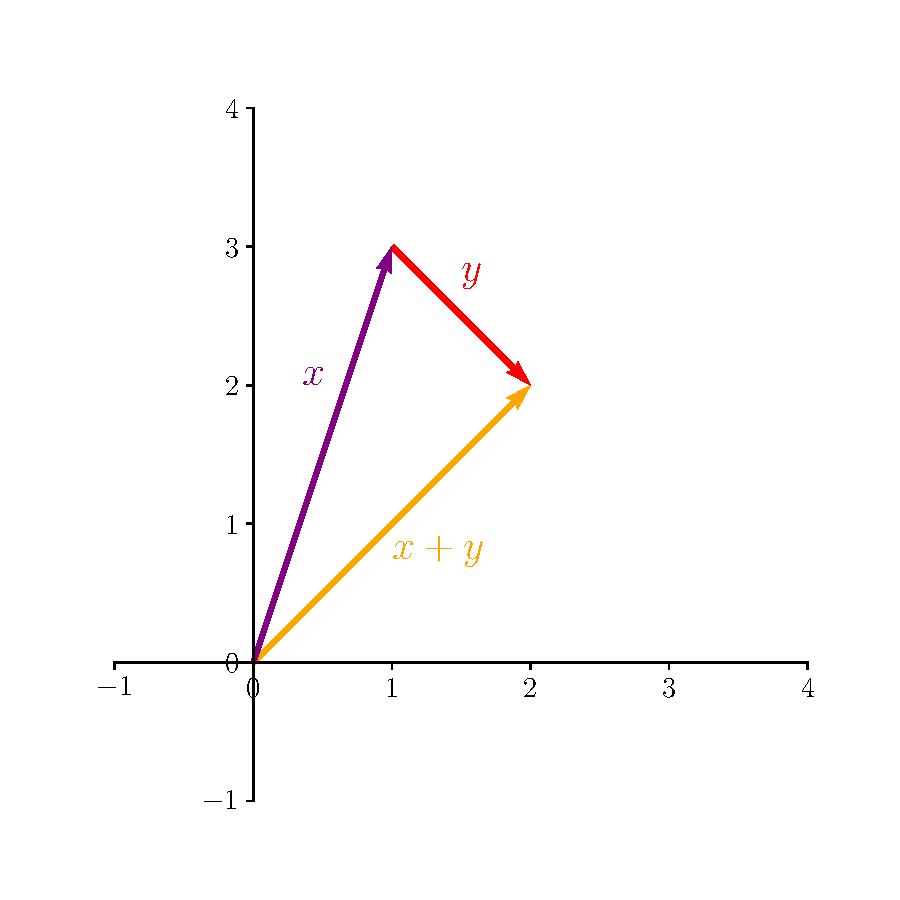
\includegraphics[width=0.4\linewidth]{figure/eps/TrangleIneq.eps}
	\caption{三角不等式}
	\label{fig:TrangleIneq}
\end{figure}

\begin{axiom}{平面长度最短公理}
	在平面内,两点之间,线段最短。
\end{axiom}

如果将其推广到内积空间,则有如下不等式成立:

\begin{theorem}{三角不等式}
	若$u,v\in H$,则$$\left \| u+v \right \| \le \left \| u \right \| +\left \| v \right \| $$当且仅当$u=\lambda v,\lambda>0$等号成立。
\end{theorem}

\begin{proof}
	首先根据范数的定义,我们可以得到$$\left \| u+v \right \|^2 =\left \langle u+v,u+v \right \rangle $$根据两个变量的线性,我们可以得到$$\left \langle u+v,u+v \right \rangle =\left \langle u,u \right \rangle +\left \langle v,v \right \rangle +\left \langle u,v \right \rangle +\left \langle v,u \right \rangle $$根据共轭对称性可得$$\left \langle u+v,u+v \right \rangle =\left \langle u,u \right \rangle +\left \langle v,v \right \rangle +\left \langle u,v \right \rangle +\overline{\left \langle u,v \right \rangle} $$化简并合并可得$$\left \| u+v \right \|^2=\left \| u \right \| ^2+\left \| v \right \| ^2+2\text{Re}\left \langle u,v \right \rangle \footnote{若$x=a+b\mathrm{i}$那么$\text{Re}(x)$表示取$x$的实数部分$a$,$\text{Im}(x)$表示取$x$的虚数部分$b$}$$适当取放缩可得$$\left \| u+v \right \|^2\le \left \| u \right \| ^2+\left \| v \right \| ^2+2\left | \left \langle u,v \right \rangle  \right | $$根据Cauchy-Schwarz不等式可得$$\left \| u \right \| ^2+\left \| v \right \| ^2+2\left | \left \langle u,v \right \rangle  \right | \le \left \| u \right \| ^2+\left \| v \right \| ^2+2\left \| u \right \|\left \| v \right \|$$最后我们合并不等式右侧,可得$$\left \| u+v \right \|^2 \le \left( \left \| u \right \| +\left \| v \right \|  \right)^2$$
	两边开二次根即可得证。$\square$
\end{proof}

\section{正交}

\subsection{正交的定义}

根据内积公式$\left \langle u,v \right \rangle =\left \| u \right \| \left \| v \right \| \cos \varphi$,特别地,两个向量的内积等于0的时候我们有一个关键的定义:正交。

\begin{definition}{正交(orthogonal)的定义}
	若向量$a,b \in H$有$\left \langle a,b \right \rangle = 0$则称$a,b$是正交的\footnote{有些教材会使用$a,b$是垂直的}。
\end{definition}

通常来讲,向量的范数不为0,当$\cos \varphi$为0的时候两个向量正交;也就是说,通常两个向量的夹角为$\displaystyle \frac{\pi}{2}$的时候两个向量正交。

对于向量$\boldsymbol{0}$我们有如下推论:

\begin{corollary}
	\begin{enumerate}
		\item $\boldsymbol{0}$与$H$中的任何向量正交;
		\item $\boldsymbol{0}$与自身正交。
	\end{enumerate}
\end{corollary}

\subsection{正交基}

首先是正交基的概念,若基集合$\left\{ a_1,a_2,a_3\cdots,a_n \right\}$是正交基,则该基的元素两两正交。

\begin{definition}{正交基(orthonormal basis)}
	若内积空间$H$上的基$S=\left\{ a_1,a_2,a_3\cdots,a_n \right\}$满足对于任意一个$i,j \in \mathbb{N}^+$且$i\neq j$使得$$\left \langle a_i,a_j \right \rangle =0$$我们称$S$为空间$H$的正交基。
\end{definition}

举个例子,$\mathbb{R}^3$的正交基可以是$\left\{ (0,0,1),(0,1,0),(1,0,0) \right\}$。

\subsection{Gram-Schmidt 正交化}

在前面的学习中,若线性空间$V$的基为$S=\left\{ a_1,a_2,a_3,\cdots,a_n \right\}$那么对于任意一个$v\in V$都可以使用$S$的线性组合表示,即对于任何一个$v \in V$存在$\lambda_1,\lambda_2,\lambda_3,\cdots,\lambda_n$满足下面的式子成立。$$v=\lambda_1a_1+\lambda_2a_2+\lambda_3a_3+\cdots+\lambda_na_n$$由于正交基是一种特殊的基,所以它们也满足该性质,我们有如下的等式来描述它们的线性组合表示的向量,称作正交分解。

\begin{theorem}{正交分解(orthogonal decomposition)}
	\label{the:orthogonalDecomposition}
	设内积空间$V$上的基为$S=\left\{ a_1,a_2,a_3,\cdots,a_n \right\}$,则对于任何一个$v\in V$满足等式$$v=\left \langle v,a_1 \right \rangle a_1+\left \langle v,a_2 \right \rangle a_2+\cdots+\left \langle v,a_n \right \rangle a_n$$成立,写成求和符号就是$$v=\sum_{i=1}^{n} \left \langle v,a_i \right \rangle a_i$$并同时满足$$\left \| v \right \| ^2=\sum_{i=1}^{n}\left( \frac{\left | \left \langle v,a_i \right \rangle  \right |}{\left \| a_i \right \|} \right)^2$$
\end{theorem}

我们还是从$\mathbb{R}^2$和$\mathbb{R}^3$入手考虑,通常在我们高中的物理学习中会学到力的分解,下面是在$\mathbb{R}^2$上的图形直观的解释。

\begin{figure}[htbp]
	\centering
	
\begin{tikzpicture}[yscale=1,xscale=1,line width=0.8pt]
    \draw (0,0) rectangle (4,2);
    \draw[->,>=Stealth] (2,1)--(6,3)node[above=2.5pt,right=2.5pt]{$F$};

	\draw[->,>=Stealth,dashed] (2,1)--(2,3)node[above=2.5pt,right=2.5pt]{$F_{\text{垂直}}$};

    \draw[->,>=Stealth,dashed] (2,1)--(6,1)node[above=2.5pt,right=2.5pt]{$F_{\text{平行}}$};

    \coordinate (O) at (2,1);
    \coordinate (A) at (3,1.5);
    \coordinate (B) at (3,1);
    \draw pic["$\varphi$",draw,angle radius=1cm,angle eccentricity=1.4] {angle = B--O--A};
\end{tikzpicture}
	\caption{力的合成与分解}
	\label{tikz:force}
\end{figure}

如图\ref{tikz:force}所示,$F_{\text{垂直}}$和$F_{\text{平行}}$是正交的,我们可以将$F$分解为这两个向量,根据内积公式,$\left \langle F,F_{\text{平行}} \right \rangle =\left \| F \right \| \left \| F_{\text{平行}} \right \|\cos \varphi $所以分解为$F_{\text{平行}}$的分量可以使用正交分解公式,同理$F_{\text{垂直}}$也是如此,这样一来可以将$F$分解为两个正交基的和即$$F=F_{\text{垂直}}+F_{\text{平行}}$$

同理,在$\mathbb{R}^n$上的向量均可使用定理\ref{the:orthogonalDecomposition}使其正交化;而下面要讲的一个内容表示的是,可以将一些线性无关的向量正交化,使其两两正交。且正交化后张成的空间与原向量张成的空间相同,这就是 Gram-Schmidt\footnote{一般译作格拉姆-施密特,由两位数学家的名字构成,分别是丹麦数学家Jørgen Pedersen Gram和德国数学家Erhard Schmidt} 正交化过程。
%cite

\begin{theorem}{Gram-Schmidt 正交化}
	设向量$S=\left\{ v_1,v_2,v_3,\cdots,v_n \right\}$线性无关,存在向量$S'=\left\{ a_1,a_2,a_3,\cdots,a_n \right\}$为正交基,并满足
	$$a_k=v_k-\sum_{i=1}^{k-1} \frac{\left \langle a_i,v_k \right \rangle }{\left \langle a_i,a_i \right \rangle }a_i $$
	成立,且$$\text{Span}(S)=\text{Span}(S')$$
\end{theorem}

下面是一个利用 Gram-Schmidt 正交化的一个例子。

\begin{example}
	在三维空间$\mathbb{R}^3$中,有一组基$\left\{ a_1,a_2,a_3 \right\}$,其中$a_1=(1,1,1),a_2=(1,1,0),a_3=(1,0,0)$请使用 Gram-Schmidt 正交化将其转化为$S'=\left\{ v_1,v_2,v_3 \right\}$,$S'$为$\mathbb{R}^3$的正交基。
	\tcblower
	\textcolor{purple}{\textbf{解}}:根据 Gram-Schmidt 正交化依次可得\begin{align}
		&v_1=a_1=(1,1,1)\\&v_2=a_2-\frac{\left \langle v_1,a_1 \right \rangle }{\left \langle v_1,v_1 \right \rangle }v_1=(0,1,1)-\frac{2}{3}(1,1,1)=\left( -\frac{2}{3},\frac{1}{3},\frac{1}{3} \right)\\&v_3=a_3-\frac{\left \langle v_1,a_3 \right \rangle }{\left \langle v_1,v_1 \right \rangle }v_1-\frac{\left \langle v_2,a_3 \right \rangle }{\left \langle v_2,v_2 \right \rangle }v_2\notag\\&v_3=(0,0,1)-\frac{1}{3}(1,1,1)-\frac{1/3}{2/3}\left( -\frac{2}{3},\frac{1}{3},\frac{1}{3}  \right)=\left( 0,-\frac{1}{2},\frac{1}{2} \right)
	\end{align}
\end{example}

\begin{ascolorbox1}{思考}
	如果向量$S$线性相关,如果对其使用 Gram-Schmidt 正交化会发生什么?
\end{ascolorbox1}

答案是最后一个向量正交化后会变为$\boldsymbol{0}$向量,它们确实两两正交,不过$\boldsymbol{0}$向量不能成为基的一个。

读者不难发现,向量在正交化的时候也相当于一个线性映射,即原向量$v_i$被映射为了$a_i$,同时也不难发现这是一个从自己空间映射到自己空间的映射,我们给它一个名称叫做算子(operator)。

\begin{definition}{算子(operator)}
	线性映射从$V$到$V$的集合$\mathcal{L}(V,V)$中的元素称作$V$上的算子,我们把线性映射到本身的集合简写为$\mathcal{L}(V)$。
\end{definition}

例如线性映射,$T((x,y))=(y,x)$,$T$就是$\mathbb{R}^2$上的算子,因为映射前后的空间都是$\mathbb{R}^2$,可以写作$T\in \mathcal{L}(\mathbb{R}^2)$。

回到刚刚所说的原向量$v_i$被映射为了$a_i$,若映射法则$T$将$v_i$被映射为了$a_i$,如果我们将此线性映射表示为矩阵积,那么它应当满足:$$\begin{pmatrix}
	a_1& a_2 & a_3 & \cdots & a_n
  \end{pmatrix}=\begin{pmatrix}
	v_1& v_2 & v_3 & \cdots & v_n
\end{pmatrix}\mathcal{M}(T)\footnote{这种写法用向量的矩阵表示,即若$a_i,v_i\in \mathbb{R}^m$则这两个是$m\times n$的矩阵}$$在正交化这样的过程中,我们可以得到$\mathcal{M}(T)$是上三角矩阵,即$$\begin{pmatrix}
	a_1& a_2 & a_3 & \cdots & a_n
  \end{pmatrix}=\begin{pmatrix}
	v_1& v_2 & v_3 & \cdots & v_n
	\end{pmatrix}=\begin{pmatrix}  
	1 & * & \cdots &* & * \\  
	0 & * & \cdots &* & * \\  
	\vdots & \vdots & \ddots & \vdots & \vdots \\  
	0 & 0 & \cdots & 0 & * 
  \end{pmatrix} $$

\subsection{正交投影}

想象一下在$\mathbb{R}^3$中,有一条直线和一个平面垂直,在高中的学习生涯中我们知道在平面上任意取一个有向箭头,都与这条直线垂直,换句话说,平面上所有有向箭头表示的向量都与这条直线的方向向量正交。

所以我们引入一个正交补空间,表示该空间内向量对一个子空间中的任意一个向量正交,下面我们给出定义:

\begin{definition}{正交补空间}
	设子空间$U$中的向量均与子空间$V$中的向量正交,我们称$V$是$U$的正交补空间,并有一个符号$U^{\bot}$表示;即$$U^{\bot}:=\left\{ a\in V\mid \forall\footnote{符号$\forall$ 表示对于所有的,这个集合的描述为,$U^{\bot}$集合的元素$a\in V$对于所有的$u \in U$的使得$\left \langle u,a \right \rangle =0$成立} u\in U\Longrightarrow \left \langle u,a \right \rangle =0 \right\}$$
\end{definition}

\begin{figure}[htbp]
	\centering
	\tdplotsetmaincoords{70}{100}

\begin{tikzpicture}[yscale=1,xscale=1,line width=0.8pt,tdplot_main_coords]
	\coordinate (A) at (0,0,0);
	\coordinate (B) at (4,0,0);
    \coordinate (C) at (4,4,-2);
    \coordinate (D) at (0,4,-2);

    \coordinate (L1) at (2,3,1);
    \coordinate (L2) at (2,1,-3);

    \draw (L1)--(L2) node[above=3.5pt,right=3pt]{$l$};
    
    \fill[pink!40!white,opacity=0.6] (A)--(B)--(C)--(D)--cycle;
    \draw (B)node[above=3.5pt,right=3pt]{$\alpha$};
	%\draw(P)node[above=3.5pt,right=3pt]{$P$};
\end{tikzpicture}
	\caption{正交补空间}
	\label{tikz:botspace}
\end{figure}

如图\ref{tikz:botspace}所示,$\mathbb{R}^3$上满足$l \bot \alpha$所以$l$和$\alpha$表示的线性空间相互正交补,即$\alpha^{\bot}=l,l^{\bot}=\alpha$,由此我们引入正交投影的概念,并解决一些极小化问题。

\begin{definition}{正交投影(orthogonal projection)}
	设$V$的一个有限维子空间为$U$,定义$V$到$U$上的正交投影为$P_{U}\in \mathcal{L}(V)$为对所有的$v\in V$均可写成$v=u+w$,其中$u\in U$且$w\in U^{\bot}$,则$P_U(v)=w$,向量$w$称为$v$在$U$上的投影。
\end{definition}

结合我们之前讲过的线性映射的零空间和值域空间,便有如下推论。

\begin{corollary}
	若$U$是$V$的有限维子空间,则$P_U\in \mathcal{L}(V)$满足$$\text{range}P_U=\left( \text{null} P_U \right)^{\bot}=U$$
\end{corollary}

\section{极小化问题}

\subsection{到子空间的最短距离}

还是在高中的学习生涯中我们遇到过在空间$\mathbb{R}^3$上给定一个点,并求它到直线或平面的最短距离,为了后续抽象化的操作,我们先来定义什么是点。

\begin{definition}{点(point)与点的距离(point distance)}
	子空间$V$上的点$v\in V$是一个向量,在图形中通常表示为从 $\boldsymbol{0}$开始的有向箭头。若两个不相同的点$v,w \in V$则它们的距离表示为$$d(v,w) := \left \| v-w \right \| \footnote{在这一部分,我们都用欧几里得体系表示空间}$$
\end{definition}

例如在$\mathbb{R}^2$中点$v=(3,4)$和点$w=(0,1)$的距离为$d(v,w)=\sqrt{3^2+3^2}=3\sqrt{2}$,根据定义我们可以把上面的问题描述成:给定一个空间$V$的子空间$U$和点$v\in V$,求点$u\in U$使得$\left \| v-u \right \| $最小;在解决该问题的策略中,我们知道点到直线或平面的距离最短的情况应该是垂直到点的情形,所以到子空间的最小距离应当是到该子空间正交补空间上取点,下面的一个命题表示将点通过$P_U$映射到子空间后点的距离最短。

\begin{theorem}{到子空间的最短距离}
	设$U$为$V$有限维子空间,有$v\in V$且$u\in U$那么$$\left \| v-P_U(v) \right \| \le \left \| v-u \right \| $$
\end{theorem}

\begin{figure}[htbp]
	\centering
	\begin{tikzpicture}[yscale=1,xscale=1,line width=0.8pt]
	\coordinate (A) at (-1,-1);
	\coordinate (B) at (4,4);
    \coordinate (O) at (0,0);
    \coordinate (V) at (1,3);
    \coordinate (P) at (2,2);
    \draw (A)--(B) node[above=3.5pt,right=3pt]{$U$};
    \draw[->,>=Stealth](O)--(V)node[above=2.5pt,left=1.5pt]{$v$};
    \draw[->,>=Stealth](O)--(P)node[above=2.5pt,right=1.5pt]{$P_U(v)$};
    \filldraw[black] (O) circle (2pt) node[anchor=west]{$O$};
    \draw (P)--(V);
	%\draw(P)node[above=3.5pt,right=3pt]{$P$};
\end{tikzpicture}
	\caption{$P_U(v)$是$v$的最短距离}
	\label{tikz:botDistanceLine}
\end{figure}

如图\ref{tikz:botDistanceLine}所示,将$v$正交投影到$U$上的$P_U$点,它们距离最短。

\subsection{多项式与最小化}

首先我们给出两个函数内积的定义。

\begin{definition}{函数的内积}
	定义区间$S=\left[ a,b \right]$上的连续实值函数构成的的向量可定义内积如下:
	$$\left \langle f,g \right \rangle =\int_{a}^{b} f(x)g(x)\mathrm{d}x $$
\end{definition}

下面将以此介绍一个最小化方法,求解一些函数的多项式近似。在之前微积分的学习中,我们学到了麦克劳林近似,它在0处对函数有着极好的逼近。

\begin{theorem}{麦克劳林近似}
	函数$f(x)$的$n$阶导数为$f^{(n)}(x)$满足公式$$f(x)=f(0)+f'(0)x+\frac{f''(0)}{2!}x^2+\cdots+\frac{f^{(0)}}{n!}x^n+\frac{f^{(n+1)}(\theta x)}{(n+1)!}x^{n+1}(0<\theta<1)$$
\end{theorem}

下面我们新介绍一个方法叫做 Legendre 多项式,利用正交的极小化完成对函数的多项式近似,为了形成对比,我们先使用泰勒近似取最高次数项为 5 次的结果$$\sin x\sim x-\frac{x^3}{3!}+\frac{x^5}{5!}$$根据 Python-Matplotlib 工具我们绘制了这样的图:

\begin{figure}[htbp]
	\centering
	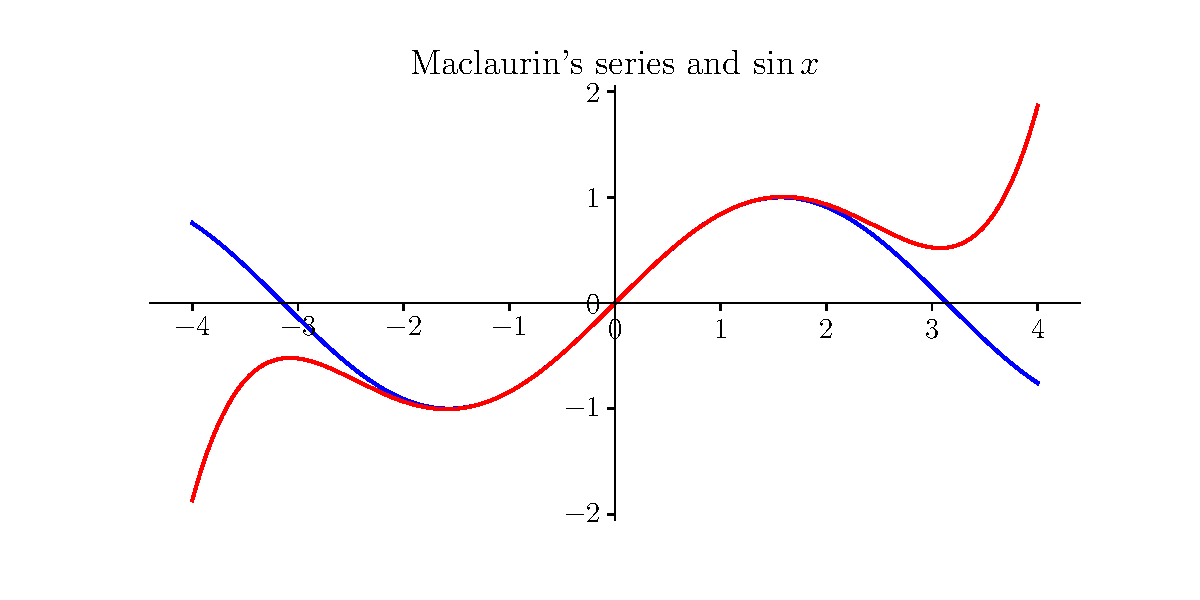
\includegraphics[width=0.7\linewidth]{figure/eps/FunctionPolMaclaurin.eps}
	\caption{蓝色为$\sin x$的图像,红色为麦克劳林近似多项式}
	\label{fig:Maclaurin}
\end{figure}

接下来使用正交最小化的方式来取近似,首先我们令多项式为函数$g(x)$设函数$f(x)=\sin x$与函数$g(x)$在$\left[ -\pi,\pi \right]$的内积表示为$$\left \langle f,g \right \rangle =\int_{-\pi}^{\pi} f(x)g(x)\mathrm{d}x $$下面选取$u(x)$的基$\left\{ 1,x,x^2,x^3,x^4,x^5 \right\}$对其使用Gram-Schmidt正交化,设$\left\{ v_0,v_1,v_2,v_3,v_4,v_5 \right\}$为正交化过程后的基,我们有:
\begin{align}
	&v_0=1\\
	&v_1=x-\frac{\left \langle x,v_0 \right \rangle }{\left \langle v_0,v_0 \right \rangle }v_0=x\\
	&v_2 = x^2 - \frac{\langle x^2, v_0 \rangle}{\langle v_0, v_0 \rangle} v_0 - \frac{\langle x^2, v_1 \rangle}{\langle v_1, v_1 \rangle} v_1\\&\cdots\notag
\end{align}
重复采用函数内积公式将对空间$U=\left\{ v_0,v_1,v_2,v_3,v_4,v_5 \right\}$和函数空间$f(x)=\sin x$计算$P_U(f)$,计算$P_U(f)$表示函数空间$$g(x)=0.987862x-0.155271x^3+0.00564312x^5$$%cite、

如果你使用的是电子介质,你可以放大并看到它们拟合的几乎严丝合缝,相较于麦克劳林近似,这种近似法在 3 处仅有微小差别。而麦克劳林近似由于采用的在0处展开,所以越靠近0,拟合的效果越好,下面给出一张表来观察两种近似的对比:

如图表所示,麦克劳林近似在越靠近0处的拟合效果更好,而纵观全局,Legendre 多项式近似法在$\left[ -\pi,\pi \right]$上拟合效果更好。正交投影最小化帮我们找到了一个方法,改进了我们在微积分学习中学到的近似。实际上,如果我们给定一个函数如下$$\mathcal{F}(x)=\int_{-\pi}^{\pi} \left | \sin x-u(x) \right |^2 \mathrm{d}x $$这个函数表示在拟合过程中,多项式函数与被拟合函数相减并平方围成的面积,这个值越小,在这种情况下拟合效果越好,实际上,使用 Legendre 多项式近似法要比麦克劳林近似,该值要小得多。

\begin{figure}[htbp]
	\centering
	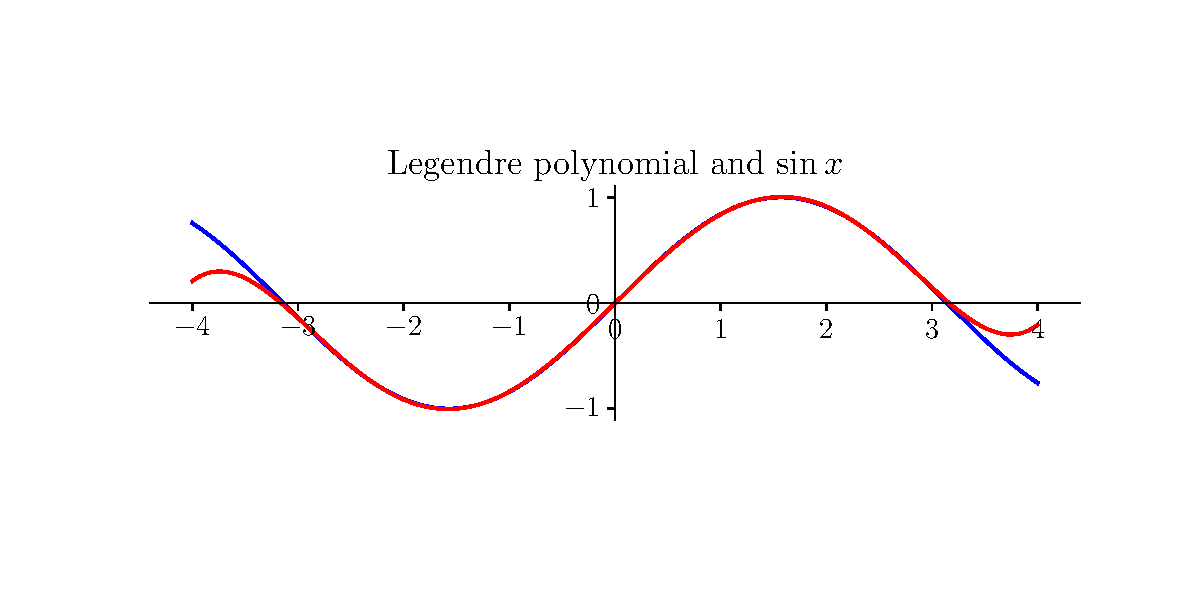
\includegraphics[width=0.7\linewidth]{figure/eps/FunctionPolLegendre.eps}
	\caption{蓝色为$\sin x$的图像,红色为 Legendre 多项式近似法}
	\label{fig:PolLegendre}
\end{figure}

\begin{table}
	\centering
	\begin{minipage}[c]{\textwidth}
		% Please add the following required packages to your document preamble:
% \usepackage[table,xcdraw]{xcolor}
% Beamer presentation requires \usepackage{colortbl} instead of \usepackage[table,xcdraw]{xcolor}

\centering
\caption{Legendre 多项式近似与麦克劳林近似的数值比较}
\begin{tabular}{|
>{\columncolor[HTML]{EAECF0}}l |l|l|l|}
\hline
        & \cellcolor[HTML]{EAECF0}$\sin x$ & \cellcolor[HTML]{EAECF0}Legendre 多项式近似 & \cellcolor[HTML]{EAECF0}麦克劳林近似 \\ \hline
$x=0$   & 0.0                              & 0.0                                    & 0.0                            \\ \hline
$x=1/3$ & 0.3271946967961522               & 0.3235597782716049                     & 0.3271947873799726             \\ \hline
$x=2/3$ & 0.618369803069737                & 0.6133115713580247                     & 0.6183813443072702             \\ \hline
$x=1$   & 0.8414709848078965               & 0.8382341200000001                     & 0.8416666666666667             \\ \hline
$x=4/3$ & 0.9719379013633127               & 0.9728796167901235                     & 0.9733882030178327             \\ \hline
$x=5/3$ & 0.9954079577517649               & 1.0001604320987654                     & 1.0022290809327847             \\ \hline
$x=2$   & 0.9092974268256817               & 0.9141358400000001                     & 0.9333333333333333             \\ \hline
$x=7/3$ & 0.7230858817383246               & 0.7227987441975305                     & 0.7924211248285326             \\ \hline
$x=8/3$ & 0.457272626635812                & 0.4508624039506175                     & 0.6299039780521267             \\ \hline
$x=3$   & 0.1411200080598672               & 0.14254716000000012                    & 0.5249999999999999             \\ \hline
\end{tabular}

	\end{minipage}
\end{table}

\section{章节练习}

\subsection{A组}

\begin{reidai}
	设$V$为实内积空间,尝试证明极化恒等式成立,即对$v,w\in V$有$$\left \langle v,w \right \rangle =\frac{\left \| v+w \right \|^2-\left \| v-w \right \|^2  }{4}$$
\end{reidai}

\begin{reidai}
	设$v,w\in V$,若$\left \| v \right \| =3, \left \| v+w \right \| =4, \left \| v-w \right \| =6$求$\left \| w \right \| $的值。
\end{reidai}

\begin{reidai}
	请自行选取一个关于$\mathbb{R}^4$的非正交基,使用 Gram-Schmidt 正交化将其转化为正交基。
\end{reidai}

\begin{reidai}
	证明,菱形的对角线相互垂直,即对角线表示的有向箭头正交。
\end{reidai}

\begin{reidai}
	比较大小:设数列$\left\{ a_n \right\}$,比较它们的平均数的平方的和与它们和的平方的平均数的大小,即$$\frac{1}{n} \left ( \sum_{i=0}^{n}a_i^2  \right ) \quad \text{and} \quad \left ( \frac{1}{n} \left ( \sum_{i=1}^{n}a_i \right )  \right )  ^2$$
\end{reidai}

\begin{reidai}
	若基$S=\left\{ (1,2,3,4),(9,8,7,6) \right\}$其张成空间为$\text{Span}(S)=U$为$\mathbb{R}^4$的子空间,求$U$的一个正交基和$U^{\bot}$的一个正交基。
\end{reidai}

\begin{reidai}
	若基$S=\left\{ (1,1,0,0),(1,1,1,2) \right\}$其张成空间为$\text{Span}(S)=U$为$\mathbb{R}^4$的子空间,求$u\in U$的使得$\left \| u-(1,2,3,4) \right \| $最小。
\end{reidai}

\subsection{B组}

\begin{reidai}
	多项式$P(x)$的最高次数为2,在此之上考虑内积$$\left \langle f,g \right \rangle =\int_{0}^{1} f(x)g(x)\mathrm{d}x $$对基$\left\{ 1,x,x^2 \right\}$使用Gram-Schmidt正交化求$P(x)$的一个正交基。
\end{reidai}

\begin{reidai}
	请使用 Legendre 多项式与正交化,对$\ln x$在$\left [ 1,2 \right ] $上进行最高次数为 5 的多项式拟合。
\end{reidai}



\partsimage{figure/parts/2.png}
\part{基础部分}
\chapterimage{chapters/4.png}
\chapter{行列式}
\begin{center}
	% \textcolor[RGB]{255, 0, 0}{\faHeart}所以生命啊,它苦涩如歌.\textcolor[RGB]{255, 0, 0}{\faHeart}
	「鸟下绿芜秦苑夕,蝉鸣黄叶汉宫秋」
\end{center}
\rightline{——《咸阳城东楼》}
\vspace{-5pt}
\begin{center}
	\pgfornament[width=0.36\linewidth,color=lsp]{88}
\end{center}

\section{面积与体积}

\subsection{面积}

考虑在如图\ref{tikz:areaDet}所示平面直角坐标系中$u,v\in \mathbb{R}^2$,有向箭头$\overrightarrow{OA}=v=(v_1,v_2),\overrightarrow{OB}=u=(u_1,u_2),\overrightarrow{OC}=u+v$,求平行四边形$OACB$的面积。

\begin{figure}[htbp]
	\centering
	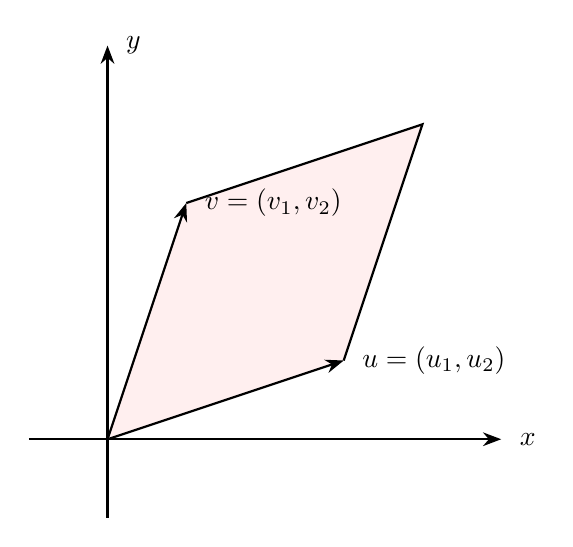
\begin{tikzpicture}[yscale=1,xscale=1,line width=0.8pt]
    \coordinate (O) at (0,0);
    \coordinate (A) at (1,3);
    \coordinate (B) at (3,1);
    \coordinate (C) at (4,4);
    \fill[pink!40!white,opacity=0.6] (O)--(A)--(C)--(B)--cycle;
    \draw[->,>=Stealth] (O)--(B) node[above=3.5pt,right=3pt]{$u=(u_1,u_2)$};
    \draw[->,>=Stealth] (-1,0)--(5,0) node[above=3.5pt,right=3pt]{$x$};
    \draw[->,>=Stealth] (0,-1)--(0,5) node[above=3.5pt,right=3pt]{$y$};
    \draw[->,>=Stealth] (O)--(A) node[above=3.5pt,right=3pt]{$v=(v_1,v_2)$};

    \draw (B)--(C)--(A);
    
    % \draw (A)--(B) node[above=3.5pt,right=3pt]{$U$};
    % \draw[->,>=Stealth](O)--(V)node[above=2.5pt,left=1.5pt]{$v$};
    % \draw[->,>=Stealth](O)--(P)node[above=2.5pt,right=1.5pt]{$P_U(v)$};
    % \filldraw[black] (O) circle (2pt) node[anchor=west]{$O$};
    % \draw (P)--(V);
	%\draw(P)node[above=3.5pt,right=3pt]{$P$};
\end{tikzpicture}
	\caption{平行四边形}
	\label{tikz:areaDet}
\end{figure}

在小时候我们没有学习过高级方法的时候,我们通常会使用割补法来计算它们的面积,通常会如下作图

\begin{figure}[htbp]
	\centering
	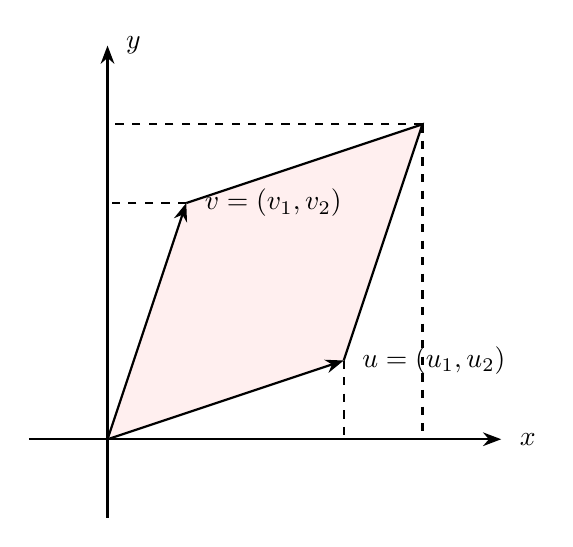
\begin{tikzpicture}[yscale=1,xscale=1,line width=0.8pt]
    \coordinate (O) at (0,0);
    \coordinate (A) at (1,3);
    \coordinate (B) at (3,1);
    \coordinate (C) at (4,4);
    \fill[pink!40!white,opacity=0.6] (O)--(A)--(C)--(B)--cycle;
    \draw[->,>=Stealth] (O)--(B) node[above=3.5pt,right=3pt]{$u=(u_1,u_2)$};
    \draw[->,>=Stealth] (-1,0)--(5,0) node[above=3.5pt,right=3pt]{$x$};
    \draw[->,>=Stealth] (0,-1)--(0,5) node[above=3.5pt,right=3pt]{$y$};
    \draw[->,>=Stealth] (O)--(A) node[above=3.5pt,right=3pt]{$v=(v_1,v_2)$};

    \draw (B)--(C)--(A);
    
    \draw[dashed] (A)--(0,3);
    \draw[dashed] (B)--(3,0);
    \draw[dashed] (C)--(0,4);
    \draw[dashed] (C)--(4,0);
    % \draw (A)--(B) node[above=3.5pt,right=3pt]{$U$};
    % \draw[->,>=Stealth](O)--(V)node[above=2.5pt,left=1.5pt]{$v$};
    % \draw[->,>=Stealth](O)--(P)node[above=2.5pt,right=1.5pt]{$P_U(v)$};
    % \filldraw[black] (O) circle (2pt) node[anchor=west]{$O$};
    % \draw (P)--(V);
	%\draw(P)node[above=3.5pt,right=3pt]{$P$};
\end{tikzpicture}
	\caption{割补法求面积}
	\label{tikz:areaDetDashed}
\end{figure}

设平行四边形面积为$S$那么$$S=(v_1+u_1)(v_2+u_2)-2u_2v_1-u_1u_2-v_1v_2=u_1v_2-u_2v_1\footnote{向量$u$在向量$v$的顺时针方向上时为正否则为负}$$所以我们可以快速地写出它们围成的平行四边形面积,即在平面直角坐标系内两个向量$u=(u_1,u_2)$和向量$v=(v_1,v_2)$围成的平行四边形面积$S$为$$S=\left| u_1v_2-u_2v_1 \right|$$

\begin{example}
	求向量$u=(3,1)$和向量$v=(1,2)$围成的平行四边形面积$S$。
	\tcblower
	\textcolor{purple}{\textbf{解}}:$S=3\times 2-1\times 1=5$
\end{example}

我们引入一个记号来表达这两个向量围成的平行四边形面积,即$$\begin{vmatrix}
	u_1&u_2 \\
	v_1&v_2
\end{vmatrix}:=u_1v_2-u_2v_1$$也称为$2\times 2$矩阵的行列式,该行列式的值的绝对值为平行四边形面积。

我们注意到该行列式由两个向量构成,如果我们尝试交换行列式的第一行和第二行,也就是交换一下围成这个四边形的向量的顺序,我们可以得到$$\begin{vmatrix}
	v_1&v_2 \\
	u_1&u_2
\end{vmatrix}:=u_2v_1-u_1v_2=-\begin{vmatrix}
	u_1&u_2 \\
	v_1&v_2
\end{vmatrix}$$读者可以将其理解为这个面积是一个带符号的面积,这个符号和两个向量顺序有关。通过观察发现,如果第二个向量在第一个向量的顺时针方向上的话,其值为正。

如果我们将某个向量放缩$\lambda$倍那么面积也会进行相对应的伸缩,即$$\lambda\begin{vmatrix}
	v_1&v_2 \\
	u_1&u_2
\end{vmatrix}=\begin{vmatrix}
	\lambda v_1& \lambda v_2 \\
	u_1&u_2
\end{vmatrix}=\begin{vmatrix}
	v_1&v_2 \\
	\lambda u_1&\lambda u_2
\end{vmatrix}$$

\subsection{体积}

考虑在三维空间$\mathbb{R}^3$中,一个直的四棱柱的面积计算公式为$S_{\text{底面积}}\times h$,考虑由图\ref{tikz:areaDet}作为空间直角坐标系的底面,从原点长出一个$z$轴后如图\ref{tikz:areaDet3d}所示。

\begin{figure}[htbp]
	\centering
	\tdplotsetmaincoords{70}{100}

\begin{tikzpicture}[yscale=1,xscale=1,line width=0.8pt,tdplot_main_coords]
    \coordinate (O) at (0,0,0);
    \coordinate (A) at (1,3,0);
    \coordinate (B) at (3,1,0);
    \coordinate (C) at (4,4,0);
    \coordinate (D) at (0,0,2);
    \fill[pink!40!white,opacity=0.6] (O)--(A)--(C)--(B)--cycle;
    \draw[->,>=Stealth] (O)--(B) node[above=3.5pt,right=3pt]{$u=(u_1,u_2,0)$};
    \draw[->,>=Stealth] (O)--(5,0,0) node[above=3.5pt,right=3pt]{$x$};
    \draw[->,>=Stealth] (O)--(0,5,0) node[above=3.5pt,right=3pt]{$y$};
    \draw[->,>=Stealth] (O)--(0,0,5) node[above=3.5pt,right=3pt]{$z$};
    \draw[->,>=Stealth] (O)--(A) node[above=3.5pt,right=3pt]{$v=(v_1,v_2,0)$};
    \draw[->,>=Stealth] (O)--(D) node[above=3.5pt,right=3pt]{$w=(0,0,w_3)$};

    \draw (B)--(C)--(A);
    \draw[dashed] (D)--(1,3,2)--(4,4,2)--(3,1,2)--(D);
    \draw[dashed] (4,4,2)--(C);
    \draw[dashed] (1,3,2)--(A);
    \draw[dashed] (3,1,2)--(B);
    % \draw (A)--(B) node[above=3.5pt,right=3pt]{$U$};
    % \draw[->,>=Stealth](O)--(V)node[above=2.5pt,left=1.5pt]{$v$};
    % \draw[->,>=Stealth](O)--(P)node[above=2.5pt,right=1.5pt]{$P_U(v)$};
    % \filldraw[black] (O) circle (2pt) node[anchor=west]{$O$};
    % \draw (P)--(V);
	%\draw(P)node[above=3.5pt,right=3pt]{$P$};
\end{tikzpicture}
	\caption{三维体积行列式表示}
	\label{tikz:areaDet3d}
\end{figure}

所以如果我们在$z$上取一个向量围成一个四棱柱,那么它的体积就是$S_{\text{底面积}}\times h$计算如图\ref{tikz:areaDet3d}的四棱柱体积为$w_3(u_1v_2-u_2v_1)$;下面引入三阶行列式,分别写三个向量来表示这个体积,即$$\begin{vmatrix}
	u_1&u_2  &0 \\
	v_1&v_2  &0 \\
	0&0  &w_3 
  \end{vmatrix}=w_3(u_1v_2-u_2v_1)$$经过割补法验证,对于$u=(u_1,u_2,u_3),v=(v_1,v_2,v_3),w=(w_1,w_2,w_3) \in \mathbb{R}^3$其张成的四棱柱体积计算公式为$$S=|u_1(v_2w_3 - v_3w_2) - u_2(v_1w_3 - v_3w_1) + u_3(v_1w_2 - v_2w_1)|$$故我们定义一个三阶行列式,表示由这三个向量构成的立方体的体积,即$$\begin{vmatrix}
	u_1& u_2 &u_3 \\
	v_1& v_2 &v_3 \\
	w_1& w_2 &w_3
  \end{vmatrix}:=u_1(v_2w_3 - v_3w_2) - u_2(v_1w_3 - v_3w_1) + u_3(v_1w_2 - v_2w_1)$$

\subsection{2或3阶行列式的性质}

前面我们定义了2,3阶的行列式,通过几何意义我们不难发现如下性质。

\begin{corollary}
	2阶,3阶行列式有如下性质
	\begin{enumerate}
		\item 行列式某几行所表示的向量线性相关,行列式值为0。
		\item 行列式某行向量乘以标量$\lambda$,行列式值也乘$\lambda$。
	\end{enumerate}
\end{corollary}

%cite 测度

我们通过图形的角度证明两个性质,第一个如果某几行向量线性相关说明三维图形会坍缩为一个平面,平面会坍缩为直线,所以它们对应的体积或面积均为0。第二个如果某行向量乘以标量$\lambda$那么它们的测度\footnote{这里的测度指的是,当描述的是一维空间其测度就是长度,二维测度为面积,三维测度为体积}也会放缩为$\lambda$倍。

\section{$n$阶行列式}

\subsection{$n$阶行列式的定义}

首先我们定义一下什么叫作$n$阶方阵。

\begin{definition}{$n$阶方阵}
	若矩阵$\mathbf{A}$是一个$m\times n$矩阵,当$m=n$时,我们称$\mathbf{A}$是$n$阶方阵
\end{definition}

例如$\mathbf{A}=\begin{pmatrix}  
	a_{11} & \cdots & a_{1n} \\  
	\vdots & \ddots & \vdots \\  
	a_{n1} & \cdots & a_{nn}  
\end{pmatrix} $表示为$n$阶方阵,我们以此定义一个数表示该方阵的行列式。

\begin{definition}{$n$阶行列式}
	定义$n$阶方阵$\mathbf{A}$的行列式为$n$阶行列式,记作$\det \mathbf{A}$,也可以记作$$\det \mathbf{A}=\begin{vmatrix}  
		a_{11} & \cdots & a_{1n} \\  
		\vdots & \ddots & \vdots \\  
		a_{n1} & \cdots & a_{nn}  
	\end{vmatrix}$$
\end{definition}

前面说到了2阶,3阶行列式,我们来讨论更一般的情况,在$n$维空间上的测度。如果我们把$\mathbb{R}^n$空间上的标准正交基$\left\{ (1,0,0,\cdots,0),(0,1,0,\cdots,0),(0,0,1,\cdots,0),\cdots,(0,0,0,\cdots,1) \right\}$放入行列式内,我们就可以得到$$\begin{vmatrix}
	1 & 0 & \cdots & 0 \\
	0 & 1 & \cdots & 0 \\
	\vdots & \vdots & \ddots & \vdots\\
	0 & 0 & \cdots & 1
\end{vmatrix}=1$$实际上,行列式的几何意义就是$n$向量张成的一个$n$维``图形''的测度。后面我们会以行展开的方式,来讲解它的运算\footnote{注意,这本书不会使用逆序排列法详细讲行列式的计算,虽然我们定义它的运算是这样的,但是这不会让我们更加理解行列式,且前面用几何法定义了它的含义,所以我们在后面的讲解中会直接讲运算方法}。

\subsection{2阶与3阶行列式的运算}

首先对于2阶行列式,计算方式肯定是:主对角线的乘积减去副对角线的乘积;对于三阶行列式,我们有如图\ref{tikz:SarrusRule}的计算记忆方法,这种方法称为 Sarrus\footnote{一般译作:萨鲁法} 法。

\begin{figure}[htbp]
	\centering
	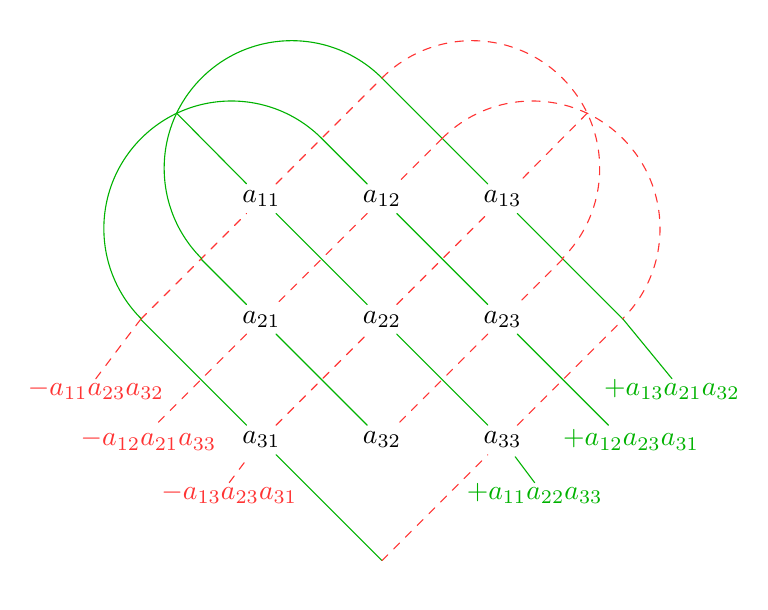
\begin{tikzpicture}[
    every node/.style = {circle,outer sep=0pt,inner sep=.1pt},
    lineleft/.style = {color = red!80,dashed,line cap=round},
    lineright/.style = {color = green!70!black,line cap=round},
    ]
    \node (node-22) {$a_{22}$};
    \node (node-21) [left = of node-22] {$a_{21}$};
    \node (node-23) [right = of node-22] {$a_{23}$};
    \node (node-12) [above = of node-22] {$a_{12}$};
    \node (node-11) [left = of node-12] {$a_{11}$};
    \node (node-13) [right = of node-12] {$a_{13}$};
    \node (node-32) [below = of node-22] {$a_{32}$};
    \node (node-31) [left = of node-32] {$a_{31}$};
    \node (node-33) [right = of node-32] {$a_{33}$};
    \node (extra-north) [above = of node-12] {\phantom{$a_{12}$}};
    \node (extra-east) [right = of node-23] {\phantom{$a_{23}$}};
    \node (extra-west) [left = of node-21] {\phantom{$a_{21}$}};
    \node (extra-south) [below = of node-32] {\phantom{$a_{32}$}};
    \node (extra-southeast) [right = of node-33] {\phantom{$a_{31}$}};
    \node (extra-southwest) [left = of node-31] {\phantom{$a_{31}$}};
    \node (M1) at ($(node-11)!.5!(extra-west)$) {};
    \node (M2) at ($(node-11)!.5!(extra-north)$) {};
    \node (N1) at ($(node-13)!.5!(extra-east)$) {};
    \node (N2) at ($(node-13)!.5!(extra-north)$) {};
    \draw[lineright] 
    (extra-north.center) -- (node-13) -- (extra-east.center)
    (M2.center) -- (node-12) -- (node-23) -- (extra-southeast)
    (node-11) -- (node-22) -- (node-33)
    (M1.center) -- (node-21) -- (node-32)
    (extra-west.center) -- (node-31) -- (extra-south.center)
    ;
    \draw[lineleft] 
    (extra-west.center) -- (node-11) -- (extra-north.center) 
    (N2.center) -- (node-12) -- (node-21) -- (extra-southwest)
    (node-31) -- (node-22) -- (node-13)
    (N1.center) -- (node-23) -- (node-32)
    (extra-south.center) -- (node-33) -- (extra-east.center)
    ;
    \draw[lineright,name path=circ1] let \p1 = ($(M2.center) - (extra-west.center)$),
        \n{radius} = {veclen(\x1,\y1)/2}
        in
        (M2.center) arc (45:225:\n{radius});
    \draw[lineright,name path=circ2] let \p1 = ($(M1.center) - (extra-north.center)$),
        \n{radius} = {veclen(\x1,\y1)/2}
        in
        (extra-north.center) arc (45:225:\n{radius});
    \draw[lineleft,name path=circ3] let \p1 = ($(N2.center) - (extra-east.center)$),
        \n{radius} = {veclen(\x1,\y1)/2}
        in
        (N2.center) arc (135:-45:\n{radius});
    \draw[lineleft,name path=circ4] let \p1 = ($(N1.center) - (extra-north.center)$),
        \n{radius} = {veclen(\x1,\y1)/2}
        in
        (extra-north.center) arc (135:-45:\n{radius});
    \draw[lineright,line cap=round,name intersections={of=circ1 and circ2}]  (intersection-1)-- (node-11);
    \draw[lineleft,line cap=round,name intersections={of=circ3 and circ4}]  (intersection-1)-- (node-13);
    \node[rectangle] (text1) [below left=.8cm of extra-west,xshift=1.05cm] {\textcolor{red!80}{$-a_{11}a_{23}a_{32}$}};
    \draw[lineleft] (text1.north) -- (extra-west.center);
    \node[rectangle,xshift=.1cm] (text2) at (extra-southwest) {\textcolor{red!80}{{$-a_{12}a_{21}a_{33}$}}};
    %\draw[lineleft] (text2.north) -- (node-21);
    \node[rectangle] (text3) [below left=.5cm of node-31,xshift=1cm] {\textcolor{red!80}{$-a_{13}a_{23}a_{31}$}};
    \draw[lineleft] (text3.north) -- (node-31);

    \node[rectangle] (text4) [below right=.8cm of extra-east,xshift=-1cm] {\textcolor{green!70!black}{$+a_{13}a_{21}a_{32}$}};
    \draw[lineright] (text4.north) -- (extra-east.center);
    \node[rectangle,xshift=.1cm] (text5) at (extra-southeast) {\textcolor{green!70!black}{$+a_{12}a_{23}a_{31}$}};
    % %\draw[lineright] (text5.north) -- (node-23);
    \node[rectangle] (text6) [below right=.5cm of node-33,xshift=-1cm] {\textcolor{green!70!black}{$+a_{11}a_{22}a_{33}$}};
    \draw[lineright] (text6.north) -- (node-33);
\end{tikzpicture}
	\caption{Sarrus 法求3阶行列式}
	\label{tikz:SarrusRule}
\end{figure}

需要注意的是只有二阶和三阶行列式具有Sarrus法则,四阶及以上的行列式不存在Sarrus法。

\section{行列式按行展开}

\subsection{代数余子式}

对于更高维度的行列式,我们通常使用按行展开的方式定义它们的运算;在此之前,我们先了解一下什么是代数余子式。

\begin{definition}{余子式与代数余子式}
	若$n$阶行列式的第$i$行第$j$列的余子式为$M_{ij}$,表示将该行与该列所有元素去除后剩下的元素将其合成为$n-1$阶行列式。而代数余子式$A_{ij}$定义为$$A_{ij}:=\left( -1 \right)^{i+j}M_{ij}$$
\end{definition}

我们用一张图来说明什么是代数余子式,若$n$阶行列式$\mathbf{D}$有$$\mathbf{D}=\begin{vmatrix}
	1 & 3 & 4 & 10\\
	2 & 5 & 9 & 11\\
	6 & 8 & 12 & 15\\
	7 & 13 & 14 & 16
\end{vmatrix}$$则它的$a_{23}$的余子式$M_{23}$为去除第二行和第三列的所有元素,留下来的成为一个3阶行列式,即$$\begin{vmatrix}
	1 & 3 & \textcolor{red}{4} & 10\\
	\textcolor{red}{2} & \textcolor{red}{5} & \textcolor{red}{9} & \textcolor{red}{11}\\
	6 & 8 & \textcolor{red}{12} & 15\\
	7 & 13 & \textcolor{red}{14} & 16
\end{vmatrix} \Longrightarrow M_{23}=\begin{vmatrix}
	1 & 3 & 10\\
	6 & 8 & 15\\
	7 & 13 & 16
\end{vmatrix},A_{23}=\left( -1 \right)^{2+3}M_{23}=-M_{23}$$

\subsection{行列式按行展开}

介绍完余子式后,我们使用 Laplace\footnote{一般译作拉普拉斯} 定理来计算行列式,在此之前我们先观察几何定义的三阶行列式,如果使用割补法来计算相关体积,我们有一个重要的推论,即$$\text{体积}=\text{底面积}\times \text{高}$$按照行列式的几何定义,$n$阶行列式的值定义为在$n$维空间上这些向量围成的$n$维测度,所以我们把式子抽象化,即$$n\text{维测度}=(n-1)\text{维测度}\times \text{高}$$仿照体积的算法$$\begin{vmatrix}
	u_1& u_2 &u_3 \\
	v_1& v_2 &v_3 \\
	w_1& w_2 &w_3
\end{vmatrix}:=u_1(v_2w_3 - v_3w_2) - u_2(v_1w_3 - v_3w_1) + u_3(v_1w_2 - v_2w_1)$$我们逐步建立高维空间,有 Laplace 定理如下

\begin{theorem}{Laplace 定理(第一行)}
	设行列式$\mathbf{D}$取第一行\footnote{由于我们没有讲到行列式的性质,这里暂时取第一行,实际上按照后面的行列式的性质,我们可以取任意一行或任意一列,此外,Laplace定理允许我们选择多行多列展开}所有元素$a_{11},a_{12},a_{13},\cdots,a_{1n}$以及它们的代数余子式$A_{11},A_{12},A_{13},\cdots,A_{1n}$,有$$\mathbf{D}=a_{11}A_{11}+a_{12}A_{12}+\cdots+a_{1n}A_{1n}$$写成求和符号为$$\mathbf{D}=\sum_{i=1}^{n} a_{1i}A_{1i}$$
\end{theorem}

下面我们来看一些例子。

\begin{example}
	使用Laplace定理计算行列式$$\mathbf{D}=\begin{vmatrix}
		1 & 2 & 0 & 3\\
		2 & 0 & 1 & 1\\
		1 & 5 & 3 & 6\\
		0 & -1 & 2 & 4
	\end{vmatrix}$$
	\tcblower
	\textcolor{purple}{\textbf{解}}:按第一行展开行列式为$$\mathbf{D}=a_{11}A_{11}+a_{12}A_{12}+a_{13}A_{13}+a_{14}A_{14}$$其中$a_{11}=1,a_{12}=2,a_{13}=0,a_{14}=3$代数余子式分别为\begin{align}
		A_{11}&=\begin{vmatrix}
			0 & 1 & 1\\
			5 & 3 & 6\\
			-1 & 2 & 4
		   \end{vmatrix}=-13\\
		A_{12}&=-\begin{vmatrix}
			2 & 1 & 1\\
			1 & 3 & 6\\
			0 & 2 & 4
		   \end{vmatrix}=2\\
		A_{13}&=\begin{vmatrix}
			2 & 0 & 1\\
			1 & 5 & 6\\
			0 & -1 & 4
		   \end{vmatrix}=51\\
		A_{14}&=-\begin{vmatrix}
			2 & 0 & 1\\
			1 & 5 & 3\\
			0 & -1 & 2
		   \end{vmatrix}=-25
	\end{align}
	其中三阶行列式可使用Sarrus法解决,也可以继续按行展开,我们得到$$\mathbf{D}=-13\times 1+2\times 2+51\times 0+(-25)\times 3=-84$$
\end{example}

不过在实际的做题中还有比这种方法更加简洁的方法,这里仅作演示,运算技巧会在后续的行列式的性质详细讲述。

\section{行列式的性质}

\subsection{转置}

行列式转置表示把行列进行调换,行变成列,列变成行。$$\mathbf{D} = \begin{vmatrix}
	1 & 2 & 3\\
	4 & 5 & 6\\
	7 & 8 & 9
\end{vmatrix} \Longrightarrow \mathbf{D}^{T}=\begin{vmatrix}
	1 & 4 & 7\\
	2 & 5 & 8\\
	3 & 6 & 9
\end{vmatrix}$$

\begin{corollary}
	行列式转置的转置等于其本身,即$\left( \mathbf{D}^{T} \right)^{T}=\mathbf{D}$
\end{corollary}

这个推论是显然的。

\begin{corollary}
	行列式转置的值等于其本身的值,即$\mathbf{D}^{T}=\mathbf{D}$
\end{corollary}

转置不变性说明在行列式中行和列的地位是平等的。因此行列式关于行变换的性质对于列变换也成立,此处不作证明,读者可以自己举例验证。

\subsection{其他性质}

\begin{corollary}
	把行列式的某一行乘以一个系数,则它的行列式的值也乘以同一个系数。
\end{corollary}

$$\begin{vmatrix}
	a_{11} & a_{12} & a_{13} & \cdots & a_{1n}\\
	\vdots & \vdots & \vdots & \vdots & \vdots\\
	\lambda a_{k1} & \lambda a_{k2} & \lambda a_{k2} & \cdots & \lambda a_{kn}\\
	\vdots & \vdots & \vdots & \vdots & \vdots\\
	a_{n1} & a_{n2} & a_{n3} & \cdots & a_{nn}
\end{vmatrix}=\lambda \begin{vmatrix}
	a_{11} & a_{12} & a_{13} & \cdots & a_{1n}\\
	\vdots & \vdots & \vdots & \vdots & \vdots\\
	a_{k1} & a_{k2} & a_{k2} & \cdots & a_{kn}\\
	\vdots & \vdots & \vdots & \vdots & \vdots\\
	a_{n1} & a_{n2} & a_{n3} & \cdots & a_{nn}
\end{vmatrix}$$

\begin{corollary}
	行列式任意两行(列)交换,行列式的值变为原来的相反数。
\end{corollary}

$$\begin{vmatrix}
	a_{11} & a_{12} & a_{13} & \cdots & a_{1n}\\
	\vdots & \vdots & \vdots & \vdots & \vdots\\
	a_{k1} & a_{k2} & a_{k3} & \cdots & a_{kn}\\
	\vdots & \vdots & \vdots & \vdots & \vdots\\
	a_{j1} & a_{j2} & a_{j3} & \cdots & a_{jn}\\
	\vdots & \vdots & \vdots & \vdots & \vdots\\
	a_{n1} & a_{n2} & a_{n3} & \cdots & a_{nn}
\end{vmatrix}=-\begin{vmatrix}
	a_{11} & a_{12} & a_{13} & \cdots & a_{1n}\\
	\vdots & \vdots & \vdots & \vdots & \vdots\\
	a_{j1} & a_{j2} & a_{j3} & \cdots & a_{jn}\\
	\vdots & \vdots & \vdots & \vdots & \vdots\\
	a_{k1} & a_{k2} & a_{k3} & \cdots & a_{kn}\\
	\vdots & \vdots & \vdots & \vdots & \vdots\\
	a_{n1} & a_{n2} & a_{n3} & \cdots & a_{nn}
\end{vmatrix}$$

\begin{corollary}
	行列式中的一行是另一行的倍数,行列式值为0;或构成行列式的向量线性相关,行列式值为0。
\end{corollary}

$$\begin{vmatrix}
	a_{11} & a_{12} & a_{13} & \cdots & a_{1n}\\
	\vdots & \vdots & \vdots & \vdots & \vdots\\
	\lambda a_{k1} & \lambda  a_{k2} & \lambda  a_{k3} & \cdots & \lambda  a_{kn}\\
	\vdots & \vdots & \vdots & \vdots & \vdots\\
	a_{k1} & a_{k2} & a_{k3} & \cdots & a_{kn}\\
	\vdots & \vdots & \vdots & \vdots & \vdots\\
	a_{n1} & a_{n2} & a_{n3} & \cdots & a_{nn}
\end{vmatrix}=\lambda \begin{vmatrix}
a_{11} & a_{12} & a_{13} & \cdots & a_{1n}\\
\vdots & \vdots & \vdots & \vdots & \vdots\\
a_{k1} & a_{k2} & a_{k3} & \cdots & a_{kn}\\
\vdots & \vdots & \vdots & \vdots & \vdots\\
a_{k1} & a_{k2} & a_{k3} & \cdots & a_{kn}\\
\vdots & \vdots & \vdots & \vdots & \vdots\\
a_{n1} & a_{n2} & a_{n3} & \cdots & a_{nn}
\end{vmatrix}=0$$

\begin{corollary}
	行列式的一行具有线性性。
\end{corollary}

$$\begin{vmatrix}
	a_{11} & a_{12} & a_{13} & \cdots & a_{1n}\\
	\vdots & \vdots & \vdots & \vdots & \vdots\\
	a_{k1}+b_{k1} & a_{k2}+b_{k2} & a_{k3}+b_{k3} & \cdots & a_{kn}+b_{k3} \\
	\vdots & \vdots & \vdots & \vdots & \vdots\\
	a_{j1} & a_{j2} & a_{j3} & \cdots & a_{jn}\\
	\vdots & \vdots & \vdots & \vdots & \vdots\\
	a_{n1} & a_{n2} & a_{n3} & \cdots & a_{nn}
\end{vmatrix}=\begin{vmatrix}
	a_{11} & a_{12} & a_{13} & \cdots & a_{1n}\\
	\vdots & \vdots & \vdots & \vdots & \vdots\\
	a_{k1} & a_{k2} & a_{k3} & \cdots & a_{kn}\\
	\vdots & \vdots & \vdots & \vdots & \vdots\\
	a_{j1} & a_{j2} & a_{j3} & \cdots & a_{jn}\\
	\vdots & \vdots & \vdots & \vdots & \vdots\\
	a_{n1} & a_{n2} & a_{n3} & \cdots & a_{nn}
\end{vmatrix}+\begin{vmatrix}
	a_{11} & a_{12} & a_{13} & \cdots & a_{1n}\\
	\vdots & \vdots & \vdots & \vdots & \vdots\\
	b_{k1} & b_{k2} & b_{k3} & \cdots & b_{kn}\\
	\vdots & \vdots & \vdots & \vdots & \vdots\\
	a_{j1} & a_{j2} & a_{j3} & \cdots & a_{jn}\\
	\vdots & \vdots & \vdots & \vdots & \vdots\\
	a_{n1} & a_{n2} & a_{n3} & \cdots & a_{nn}
\end{vmatrix}$$

\begin{corollary}
	把某一行乘以一个数加到另一行,行列式值不变。
\end{corollary}

$$\begin{vmatrix}
	a_{11} & a_{12} & a_{13} & \cdots & a_{1n}\\
	\vdots & \vdots & \vdots & \vdots & \vdots\\
	a_{k1} & a_{k2} & a_{k3} & \cdots & a_{kn}\\
	\vdots & \vdots & \vdots & \vdots & \vdots\\
	a_{j1} & a_{j2} & a_{j3} & \cdots & a_{jn}\\
	\vdots & \vdots & \vdots & \vdots & \vdots\\
	a_{n1} & a_{n2} & a_{n3} & \cdots & a_{nn}
\end{vmatrix}=\begin{vmatrix}
	a_{11} & a_{12} & a_{13} & \cdots & a_{1n}\\
	\vdots & \vdots & \vdots & \vdots & \vdots\\
	a_{k1}+a_{j1} & a_{k2}+a_{j2} & a_{k3}+a_{j3} & \cdots & a_{kn}+a_{jn}\\
	\vdots & \vdots & \vdots & \vdots & \vdots\\
	a_{j1} & a_{j2} & a_{j3} & \cdots & a_{jn}\\
	\vdots & \vdots & \vdots & \vdots & \vdots\\
	a_{n1} & a_{n2} & a_{n3} & \cdots & a_{nn}
\end{vmatrix}$$

\begin{corollary}
	上三角方阵的行列式是对角线元素的乘积。
\end{corollary}

$$\begin{vmatrix}  
	a_{11}& a_{12}& \cdots  & a_{1n} \\  
	0 & a_{22}& \cdots  & a_{2n} \\  
	\vdots & \vdots & \ddots & \vdots \\  
	0& 0& \cdots  & a_{nn}  
\end{vmatrix}=a_{11}a_{22}\cdots a_{nn}$$

\begin{corollary}
	设$n$阶方阵$\mathbf{A},\mathbf{B}$的行列式为$\det \mathbf{A},\det \mathbf{B}$有$\det (\mathbf{A}\mathbf{B})=\det \mathbf{A} \det \mathbf{B}$
\end{corollary}

\subsection{初等变换计算行列式}

我们可以利用上述的性质来计算行列式,上述性质的变换我们称为行列式的初等变换,下面是常用的几种初等变换:
\begin{enumerate}
	\item 将行列式的两行交换位置
	\item 将其中的一行乘一个非0常数
	\item 将其中的一行乘一个非0常数后加到另一行
\end{enumerate}
它们分别对应
\begin{enumerate}
	\item 行列式的值变为原来的相反数
	\item 行列式乘以同一个非零常数
	\item 保持不变
\end{enumerate}

\begin{example}
	计算行列式$\mathbf{D}=\begin{vmatrix}
		1 & 2 & 1\\
		0 & -3 & 4\\
		1 & 0 & 5
	\end{vmatrix}$
	\tcblower
	\textcolor{purple}{\textbf{解}}:将第1行乘$(-1)$加到第3行有
	$$\begin{vmatrix}
		1 & 2 & 1\\
		0 & -3 & 4\\
		1 & 0 & 5
	\end{vmatrix}=\begin{vmatrix}
		1 & 2 & 1\\
		0 & -3 & 4\\
		0 & -2 & 4
	\end{vmatrix}$$交换第2列与第3列
	$$\begin{vmatrix}
		1 & 2 & 1\\
		0 & -3 & 4\\
		0 & -2 & 4
	\end{vmatrix}=-\begin{vmatrix}
		1 & 1 & 2\\
		0 & 4 & -3\\
		0 & 4 & -2
	\end{vmatrix}$$第2行乘$(-1)$加到第3行$$-\begin{vmatrix}
		1 & 1 & 2\\
		0 & 4 & -3\\
		0 & 4 & -2
	\end{vmatrix}=-\begin{vmatrix}
		1 & 1 & 2\\
		0 & 4 & -3\\
		0 & 0 & 1
	\end{vmatrix}=-\left( 1\times 4 \times 1 \right)=-4$$
\end{example}

再来看一个4阶行列式的例子。

\begin{example}
	计算行列式$\mathbf{D}=\begin{vmatrix}
		1 & 2 & 0 & 4\\
		0 & 3 & -1 & 1\\
		3 & -1 & 5 & 0\\
		-2 & 0 & 1 & 1
	   \end{vmatrix}$
	\tcblower
	\textcolor{purple}{\textbf{解}}:将第1行乘$(-3)$加到第3行有
	$$\begin{vmatrix}
		1 & 2 & 0 & 4\\
		0 & 3 & -1 & 1\\
		3 & -1 & 5 & 0\\
		-2 & 0 & 1 & 1
	   \end{vmatrix}=\begin{vmatrix}
		1 & 2 & 0 & 4\\
		0 & 3 & -1 & 1\\
		0 & -7 & 5 & -12\\
		-2 & 0 & 1 & 1
	   \end{vmatrix}$$将第1行乘2加到第4行有
	   $$\begin{vmatrix}
		1 & 2 & 0 & 4\\
		0 & 3 & -1 & 1\\
		0 & -7 & 5 & -12\\
		-2 & 0 & 1 & 1
	   \end{vmatrix}=\begin{vmatrix}
		1 & 2 & 0 & 4\\
		0 & 3 & -1 & 1\\
		0 & -7 & 5 & -12\\
		0 & 4 & 1 & 9
	   \end{vmatrix}$$将第2行乘2加到第3行;第2行乘$(-1)$加到第4行有
	   $$\begin{vmatrix}
		1 & 2 & 0 & 4\\
		0 & 3 & -1 & 1\\
		0 & -7 & 5 & -12\\
		0 & 4 & 1 & 9
	   \end{vmatrix}=\begin{vmatrix}
		1 & 2 & 0 & 4\\
		0 & 3 & -1 & 1\\
		0 & -1 & 3 & -10\\
		0 & 1 & 2 & 8
	   \end{vmatrix}$$将第4行加到第3行有
	   $$\begin{vmatrix}
		1 & 2 & 0 & 4\\
		0 & 3 & -1 & 1\\
		0 & -1 & 3 & -10\\
		0 & 1 & 2 & 8
	   \end{vmatrix}=\begin{vmatrix}
		1 & 2 & 0 & 4\\
		0 & 3 & -1 & 1\\
		0 & 0 & 5 & -2\\
		0 & 1 & 2 & 8
	   \end{vmatrix}$$运算到这里,为了计算不出错,我们最好遵循一个原则,就是行列式内的元素尽量不要出现分数,否则计算会比较麻烦,为了转化为上三角行列式我们先对第1行第2列的元素凑为1,即:将第4行乘$(-1)$加到第一行,并提取系数4$$\begin{vmatrix}
		1 & 2 & 0 & 4\\
		0 & 3 & -1 & 1\\
		0 & 0 & 5 & -6\\
		0 & 1 & 2 & 8
	   \end{vmatrix}=\begin{vmatrix}
		1 & 1 & -2 & -4\\
		0 & 3 & -1 & 1\\
		0 & 0 & 5 & -2\\
		0 & 1 & 2 & 8
	   \end{vmatrix}$$再将第4行乘$(-3)$加到第2行后交换2,4行有
	   $$\begin{vmatrix}
		1 & 1 & -2 & -4\\
		0 & 3 & -1 & 1\\
		0 & 0 & 5 & -2\\
		0 & 1 & 2 & 8
	   \end{vmatrix}=\begin{vmatrix}
		1 & 1 & -2 & -4\\
		0 & 0 & -7 & -23\\
		0 & 0 & 5 & -2\\
		0 & 1 & 2 & 8
	   \end{vmatrix}=-\begin{vmatrix}
		1 & 1 & -2 & -4\\
		0 & 1 & 2 & 8\\
		0 & 0 & 5 & -2\\
		0 & 0 & -7 & -23
	   \end{vmatrix}$$算到这里同学们可以继续将其化为上三角,但是我们选择按列展开两次便捷,即$$-\begin{vmatrix}
		1 & 1 & -2 & -4\\
		0 & 1 & 2 & 8\\
		0 & 0 & 5 & -2\\
		0 & 0 & -7 & -23
	   \end{vmatrix}=-1\times 1\times \begin{vmatrix}
		5 & -2\\
		-7 & -23
	   \end{vmatrix}$$最后求得行列式值为$$\mathbf{D}=-\begin{vmatrix}
		5 & -2\\
		-7 & -23
	   \end{vmatrix}=129$$
\end{example}

\section{置换\footnote{本节选学} }

\subsection{全排列与置换}

本节内容选学。

如果有$n$个元素进行排列,那么将其全部有序排列的方案一共有$n!$种排列方式。如果我们将$n$个元素的初始排列集合称作初始集合,那么我们可以看作一个函数映射,将这个集合映射为$n!-1$中的一个,我们称该函数为置换函数;

\begin{definition}{置换函数}
	若集合$V=\left\{ 1,2,3,\cdots,n \right\}$,设映射法则$\sigma: V\rightarrow V$的一一映射称为一个$n $元置换。函数$f(x)$称为置换函数。
\end{definition}

例如置换映射$\sigma:\left\{ 1,2,3,4,5 \right\}\rightarrow \left\{ 3,1,4,2,5 \right\}$,那么函数$\sigma(1)=3,\sigma(2)=1,\cdots$。

\subsection{有向的$n$维测度}

首先我们还是看二维平面,其二维测度为面积,我们不难发现当向量$u=(u_1,u_2),v=(v_1,v_2)$,当$v$在$u$的顺时针方向上的时候面积为正,否则为负。

由此我们不妨以$n$维空间的标准基定义$n$维上向量的``旋转''方向,以此为基准形成排列,则如果有两个向量进行一次交换,那么它们进行一次置换后符号方向改变。如果上面的话有些抽象,我们不妨再拿二维空间举例;在二维空间中的标准基为$\left\{ (1,0),(0,1) \right\}$,其中如果有两个向量符合标准基的第一个和标准基的第二个的位置关系(第二个向量在第一个的顺时针方向),那么行列式值为正,否则为负。推广到高维空间中也是如此。

那么接下来我们继续探讨置换这些向量对行列式的影响,在此之前我们先对$\sigma$函数引入一个记号,表示$\sigma$置换了多少次。

\subsection{最少置换次数与$\text{sign} (\sigma)$}

首先定义最少置换次数函数。

\begin{definition}{最少置换次数}
	最少置换次数对置换映射法则$\sigma$的函数$\mathcal{R}:\sigma \rightarrow \mathbb{N}$,表示对使用映射法则$\sigma$之前的集合至少需要多少次置换以达到使用映射法则$\sigma$之后的集合\footnote{需要注意的是,这集合无序,但是映射后的集合却是一一对应,这里的集合可以看作是一个有序的数组,虽然集合讲究无序性}。
\end{definition}

下面我们来看一个例子,置换映射$\sigma:\left\{ 1,2,3,4,5 \right\}\rightarrow \left\{ 3,1,4,2,5 \right\}$,那么它的最少置换次数为3次,置换如下:首先初始状态为$$3,1,4,2,5$$第一次选择$3,1$调换顺序$$1,3,4,2,5$$接下里第二次选择$3,4$调换$$1,4,3,2,5$$最后第三次选择$2,4$调换顺序$$1,2,3,4,5$$所以$$\mathcal{R}(\sigma)=3$$事实上如果我们去掉最少二字的限定,置换次数可以是$3+2k,k\in \mathbb{N}$。

接下来我们继续定义函数$\text{sign}(\sigma)$,它表示的是映射$\sigma$的奇偶性;

\begin{definition}{奇偶置换}
	若式子$\mathcal{R}(\sigma)$的值如果为偶数,那么该置换为偶置换,否则为奇置换,另有函数$\text{sign}(\sigma)$定义为$$\text{sign}(\sigma):=(-1)^{\mathcal{R}(\sigma)}$$
\end{definition}

\subsection{行列式的排列定义}

还是这个例子:置换映射$\sigma:\left\{ 1,2,3,4,5 \right\}\rightarrow \left\{ 3,1,4,2,5 \right\}$,如果我们把它们的空间的标准基标号作为映射集合有$\sigma':\left\{ e_1,e_2,e_3,e_4,e_5 \right\}\rightarrow \left\{ e_3,e_1,e_4,e_2,e_5 \right\}$,相当于在$\mathbb{R}^5$空间中定义标准基的方向是这5维测度的方向,每个向量如果按这样的顺序(相当于二维空间的顺时针)排列的话,其测度为正;不过,我们对其进行了至少3次的置换,所以其测度应当为$\text{sign}(\sigma)=-1$。

如果我们类比2,3阶行列式的推导过程,即$$n\text{维测度}=(n-1)\text{维测度}\times \text{高}$$通过更高维的割补法,我们可以如下定义一个行列式:

\begin{definition}{行列式的排列定义}
	设$\mathbf{A}$是$n$阶方阵,设其第$i$行第$j$列的元素为$a_{ij}$那么有$$\det \mathbf{A}=\sum_{\sigma \in S_n}\text{sign} (\sigma)\prod_{i=1}^{n} a_{\left ( \sigma(i) \right )i}$$其中$S_n$表示是所有$n$ 元置换的集合,即共$n!$个的$\left\{ 1,2,3,\cdots,n \right\}$的全排列集合。
\end{definition}

下面举个例子,3阶行列式$\mathbf{D}=\begin{vmatrix}
	a_{11} & a_{12} & a_{13}\\
	a_{21} & a_{22} & a_{23}\\
	a_{31} & a_{32} & a_{33}
\end{vmatrix}$,它们的全排列共有$3!=6$种,分别映射为$$\left\{ \left\{ 1,2,3 \right\},\left\{ 1,3,2 \right\},\left\{ 2,1,3 \right\},\left\{ 2,3,1 \right\},\left\{ 3,1,2 \right\},\left\{ 3,2,1 \right\} \right\}$$那么对于每一个从集合$\left\{ 1,2,3 \right\}$置换开始求和,首先是$\sigma :\left\{ 1,2,3 \right\}\rightarrow \left\{ 1,2,3 \right\}$,则$$\text{sign}(\sigma)a_{11}a_{22}a_{23}=+a_{11}a_{22}a_{33}$$接下来是$\sigma :\left\{ 1,2,3 \right\}\rightarrow \left\{ 1,3,2 \right\}$则$$\text{sign}(\sigma)a_{11}a_{32}a_{23}=-a_{11}a_{32}a_{23}$$$$\cdots$$最终进行6次这样的操作后,我们得到多项式$$a_{11}a_{22}a_{33}-a_{11}a_{32}a_{23}-a_{21}a_{12}a_{33}+a_{21}a_{32}a_{13}\cdots$$

当然也可以按顺序从每行找不同列的元素相乘,结果都是一样的。

\section{章节练习}

\subsection{A组}

\begin{reidai}
	计算行列式$\mathbf{D}=\begin{vmatrix}
		1 & 2 & 3\\
		2 & -2 & 1\\
		6 & 1 & 0
	   \end{vmatrix}$
\end{reidai}

\begin{reidai}
	计算行列式$\mathbf{D}=\begin{vmatrix}
		1 & 1 & 2 & 2 & 0\\
		0 & 2 & -3 & -1 & 1\\
		1 & 1 & 3 & 1 & 1\\
		2 & -4 & 0 & 0 & 3\\
		1 & 7 & -1 & 0 & 2
	   \end{vmatrix}$
\end{reidai}

\begin{reidai}
	计算行列式$\mathbf{D}=\begin{vmatrix}
		1 & 2 & 3 & 4\\
		2 & 3 & 4 & 1\\
		3 & 4 & 1 & 2\\
		4 & 3 & 2 & 1
	   \end{vmatrix}$
\end{reidai}

\begin{reidai}
	矩阵$\mathbf{A}=\begin{pmatrix}
		2 & 1 & 0\\
		3 & 1 & 1\\
		0 & 2 & 0
	   \end{pmatrix}$,求$\det (3\mathbf{A})$和$\det (\mathbf{A}^2)$
\end{reidai}

\subsection{B组}

\begin{reidai}
	设数列$\left\{ F_n \right\}$为Fibonacci数列,其中$F_1=0,F_2=1,F_{n-1}+F_{n-2}=F_n,n\ge 2$证明$$F_{n+1}F_{n-1}-F_n^2=\left( -1 \right)^n$$
\end{reidai}

\chapterimage{chapters/5.png}
\chapter{初等矩阵}
\begin{center}
	% \textcolor[RGB]{255, 0, 0}{\faHeart}所以生命啊,它苦涩如歌.\textcolor[RGB]{255, 0, 0}{\faHeart}
	「只愿君心似我心,定不负相思意」
\end{center}
\rightline{——《卜算子$\cdot$我住长江头》}
\vspace{-5pt}
\begin{center}
	\pgfornament[width=0.36\linewidth,color=lsp]{88}
\end{center}

\section{线性方程组的解}

\subsection{二元线性方程组}

考虑一般的二元线性方程组\begin{numcases}{}
	a_{11}x_1+a_{12}x_2=b_1 \label{eq:1-1}\\
	a_{21}x_1+a_{22}x_2=b_2 \label{eq:1-2}
\end{numcases}按照正常的方法,我们将式\ref{eq:1-1}乘系数$a_{21}$,将\ref{eq:1-2}乘系数$a_{11}$后,用变换过的\ref{eq:1-1}减去\ref{eq:1-2}后我们可以得到$$\left( a_{11}a_{22}-a_{12}a_{21} \right)x_1=b_1a_{22}-b_2a_{12}$$我们可以得到方程的解$$x_1=\frac{\begin{vmatrix}
	b_1 & a_{12}\\
	b_2 & a_{22}
\end{vmatrix}}{\begin{vmatrix}
	a_{11} & a_{12}\\
	a_{21} & a_{22}
\end{vmatrix}}$$通过上述方法,我们可以得到$$x_2=\frac{\begin{vmatrix}
	a_{11} & b_1\\
	a_{21} & b_2
\end{vmatrix}}{\begin{vmatrix}
	a_{11} & a_{12}\\
	a_{21} & a_{22}
\end{vmatrix}}$$

\subsection{Cramer 法则}

以上面的二元线性方程组为例我们抽象出的两个解的表示方法,其中我们有系数矩阵行列式$$\mathbf{D}=\begin{vmatrix}
	a_{11} & a_{12}\\
	a_{21} & a_{22}
\end{vmatrix}$$其中常数矩阵$\mathbf{B}=\begin{pmatrix}
	b_1\\
	b_2
\end{pmatrix}$,我们将常数矩阵替换系数矩阵的第$i$列,得到$\mathbf{D}_i$行列式,例如$$\mathbf{D}_1=\begin{vmatrix}
	b_1 &a_{12}\\
	b_2 &a_{22}
   \end{vmatrix},\mathbf{D}_2=\begin{vmatrix}
	a_{11} & b_1 \\
	a_{12} & b_2
\end{vmatrix}$$最后方程组的第$i$个解为$$x_i=\frac{\mathbf{D}_i}{\mathbf{D}}$$

\begin{example}
	使用Cramer法则计算线性方程组$$\left\{\begin{matrix} 
		2x+3y+4z =3 \\  
		5x+4z=2\\
		x+3y+z=1
	  \end{matrix}\right. $$
	  \tcblower
	  \textcolor{purple}{\textbf{解}}:考虑系数矩阵行列式$$\mathbf{D}=\begin{vmatrix}
		2 & 3 & 4\\
		5 & 0 & 4\\
		1 & 3 & 1
	   \end{vmatrix}=33$$常数矩阵$$\mathbf{B}=\begin{pmatrix}
		3 \\
		2 \\
		1
		\end{pmatrix}$$使用常数矩阵替换行列式的第$i$列,我们可以得到$$\mathbf{D}_1=\begin{vmatrix}
			3 & 3 & 4\\
			2 & 0 & 4\\
			1 & 3 & 1
		   \end{vmatrix}=-6,\mathbf{D}_2=\begin{vmatrix}
			2 & 3 & 4\\
			5 & 2 & 4\\
			1 & 1 & 1
		   \end{vmatrix}=5,\mathbf{D}_3=\begin{vmatrix}
			2 & 3 & 3\\
			5 & 0 & 2\\
			1 & 3 & 1
		   \end{vmatrix}=24$$那么该方程组的三个解分别为$$x_1=\frac{\mathbf{D}_1}{\mathbf{D}}=-\frac{2}{11},x_2=\frac{\mathbf{D}_2}{\mathbf{D}}=\frac{5}{33},x_3=\frac{\mathbf{D}_3}{\mathbf{D}}=-\frac{8}{11}$$
\end{example}

\begin{ascolorbox1}{思考}
	当系数矩阵的行列式$\mathbf{D}=0$时是什么情况?
\end{ascolorbox1}

Cramer 法则的适用前提是系数矩阵的行列式值不能为0,读者可以发现若系数矩阵的行列式为0的时候会有一组方程组线性相关,其所面临的情况为有无穷多解或无解,例如$$\left\{\begin{matrix} 
	2x_1+3x_2 = 4 \\  
	4x_1+6x_2 = 8
  \end{matrix}\right. $$这种情况就是无穷多解,而$$\left\{\begin{matrix} 
	2x_1+3x_2 = 4 \\  
	4x_1+6x_2 = 9
  \end{matrix}\right. $$则是无解。

\subsection{齐次线性方程组}

齐次线性方程组是线性方程组中的一个特例,定义如下
\begin{definition}{齐次线性方程组(homogeneous linear equations)}
	齐次线性方程组指的是常数项全部为零的线性方程组,它们一般记作$$\left\{\begin{matrix} 
		a_{11}x_1+a_{12}x_2+a_{13}x_3+\cdots+a_{1n}x_n=0 \\  
		a_{21}x_1+a_{22}x_2+a_{23}x_3+\cdots+a_{2n}x_n=0 \\  
		a_{31}x_1+a_{32}x_2+a_{33}x_3+\cdots+a_{3n}x_n=0 \\
		\cdots \\
		a_{m1}x_1+a_{m2}x_2+a_{m3}x_3+\cdots+a_{mn}x_n=0
	  \end{matrix}\right. $$
\end{definition}

我们在第2章的B组练习中有提到这种方程组,先说结论,当$n>m$的时候齐次线性方程组必有非零解,在练习中,我们使用线性映射$$T(x_1,x_2,\cdots,x_n)=\left( \sum_{i=1}^{n}a_{1i}x_i,\sum_{i=1}^{n}a_{2i}x_i,\cdots,\sum_{i=1}^{n}a_{mi}x_i \right)$$这里的线性映射$T$将$\mathbb{F}^n$映射为$\mathbb{F}^m$,根据线性映射的基本定理有$$\text{dim}\mathbb{F}^n=\text{dim}~\text{null}T+\text{dim}~\text{range}T$$使得齐次线性方程组有无穷多解的充要条件是$T$不是单射;所以$\text{null}T\neq \left\{ 0 \right\}$(否则对应映射到零空间的向量只有$\boldsymbol{0}$)。

接下来我们考虑特殊的情况,当$m=n$的时候,系数矩阵的行列式$\mathbf{D}=\begin{vmatrix}  
	a_{11}& a_{12}& \cdots  & a_{1n} \\  
	a_{21}& a_{22}& \cdots  & a_{2n} \\  
	\vdots & \vdots & \ddots & \vdots \\  
	a_{m1}& a_{m2}& \cdots  & a_{mn}  
  \end{vmatrix}  
$如果我们对其使用 Cramer 法则,当$\mathbf{D}\neq 0$时,$\displaystyle x_i=\frac{\mathbf{D}_i}{\mathbf{D}}=0$有且仅有全为0解,即$x_1=x_2=\cdots=x_n=0$。那如果$\mathbf{D}= 0$则系数矩阵的几行向量线性相关,根据线性相关的向量可以通过去除$i$个向量可以得到线性无关的向量,由于$m=n,m-i<n$,所以我们得到齐次线性方程组有无穷多解。

\section{初等矩阵}

\subsection{增广矩阵}

%cite
首先需要注意的是,按照初等矩阵的定义,增广矩阵不算是初等矩阵的一种,但是因为它可以使用矩阵的初等行变化,所以笔者将其纳入初等矩阵这一节。

考虑线性方程组$$\left\{\begin{matrix} 
	a_{11}x_1+a_{12}x_2+a_{13}x_3+\cdots+a_{1n}x_n=b_1 \\  
	a_{21}x_1+a_{22}x_2+a_{23}x_3+\cdots+a_{2n}x_n=b_2 \\  
	a_{31}x_1+a_{32}x_2+a_{33}x_3+\cdots+a_{3n}x_n=b_3 \\
	\cdots \\
	a_{m1}x_1+a_{m2}x_2+a_{m3}x_3+\cdots+a_{mn}x_n=b_m
\end{matrix}\right. $$在系数矩阵的右边添上一列,这一列是线性方程组的等号右边的值,构成增广矩阵,记作$\tilde{\mathbf{A} } $

\begin{definition}{增广矩阵(augmented matrix)}
	线性方程组$$\left\{\begin{matrix} 
		a_{11}x_1+a_{12}x_2+a_{13}x_3+\cdots+a_{1n}x_n=b_1 \\  
		a_{21}x_1+a_{22}x_2+a_{23}x_3+\cdots+a_{2n}x_n=b_2 \\  
		a_{31}x_1+a_{32}x_2+a_{33}x_3+\cdots+a_{3n}x_n=b_3 \\
		\cdots \\
		a_{m1}x_1+a_{m2}x_2+a_{m3}x_3+\cdots+a_{mn}x_n=b_m
	\end{matrix}\right. $$其系数构成一个矩阵后在最后一列添加系数矩阵,记作$\tilde{\mathbf{A}}$,即$$\tilde{\mathbf{A}}:=\begin{pmatrix}  
		a_{11}& a_{12}& \cdots  & a_{1n} & b_1 \\  
		a_{21}& a_{22}& \cdots  & a_{2n} & b_2\\  
		\vdots & \vdots & \ddots & \vdots \\  
		a_{m1}& a_{m2}& \cdots  & a_{mn} & b_m
	  \end{pmatrix}  
	  $$
\end{definition}

通过增广矩阵的初等变换,我们可以求解线性方程组,通常这个方法叫做高斯消元法,接下里我们看一个例子:

\begin{example}
	写出线性方程组$$\left\{\begin{matrix} 
		x+y+z=4 \\  
		2x+4y+5z=16 \\
		x+5y-3z=0
	\end{matrix}\right. $$的增广矩阵
	\tcblower
	\textcolor{purple}{\textbf{解}}:见下讲解
\end{example}

我们提取该方程组的增广矩阵,即$$\tilde{A}=\begin{pmatrix}
	1 & 1 & 1 & 4\\
	2 & 4 & 5 & 16\\
	1 & 5 & -3 & 0
\end{pmatrix}$$应用矩阵的初等\textcolor{red}{行}变换就可以求解该线性方程组,下面先讲解一下什么是矩阵的初等变换。

\subsection{矩阵的初等变换}

首先为了说明变换后的矩阵和原矩阵的关系,我们使用``等价''来描述它们,需要注意的是,它们通常并不相等。设矩阵$\mathbf{A}$经过初等变换后变为$\mathbf{A}'$,则$\mathbf{A}$与$\mathbf{A}'$等价,记作$$\mathbf{A}\Longrightarrow  \mathbf{A}'$$如无特殊说明,我们这里都使用初等行变换,实际上对矩阵的列进行变换操作在某些情况下也是等价的。

\subsubsection{交换两行}

交换两行是矩阵的初等变换,例如$$\begin{pmatrix}
	1 & 3 & 3 & 3\\
\textcolor{blue}{2} & \textcolor{blue}{2} & \textcolor{blue}{2} & \textcolor{blue}{1}\\
	\textcolor{red}{4} & \textcolor{red}{2} & \textcolor{red}{1} & \textcolor{red}{3}
\end{pmatrix}\Longrightarrow \begin{pmatrix}
	1 & 3 & 3 & 3\\
	\textcolor{red}{4} & \textcolor{red}{2} & \textcolor{red}{1} & \textcolor{red}{3}\\
	\textcolor{blue}{2} & \textcolor{blue}{2} & \textcolor{blue}{2} & \textcolor{blue}{1}
\end{pmatrix}$$

\subsection{某一行乘以常数k}

某一行乘以常数$k$是矩阵的初等变换,例如$$\begin{pmatrix}
	1 & 2 & 3 & 1\\
	\textcolor{red}{4} & \textcolor{red}{2} & \textcolor{red}{1} & \textcolor{red}{2}\\
	2 & 2 & 2 & 1
\end{pmatrix}\Longrightarrow  \begin{pmatrix}
	1 & 2 & 3 & 1\\
	\textcolor{red}{4k} & \textcolor{red}{2k} & \textcolor{red}{k} & \textcolor{red}{2k}\\
	2 & 2 & 2 & 1
\end{pmatrix},k\in \mathbb{C}$$

\subsection{某个数乘以某一行并加到另一行中去}

某个数乘以某一行并加到另一行中去是矩阵的初等变换,例如$$\begin{pmatrix}
	\textcolor{red}{1} & \textcolor{red}{2} & \textcolor{red}{3} & \textcolor{red}{4}\\
	1 & 2 & 2 & 4\\
	2 & 3 & 4 & 5\\
	4 & 5 & 6 & 7
\end{pmatrix}\Longrightarrow  \begin{pmatrix}
	\textcolor{red}{1} & \textcolor{red}{2} & \textcolor{red}{3} & \textcolor{red}{4}\\
	1 & 2 & 2 & 4\\
	2+\textcolor{red}{2} & 3+\textcolor{red}{4} & 4+\textcolor{red}{6} & 5+\textcolor{red}{8}\\
	4 & 5 & 6 & 7
\end{pmatrix}$$

\subsubsection{最简矩阵}

矩阵经过一定的初等变换,可化简为最简矩阵,在给出最简矩阵的定义之前,先给出一个术语来描述一个特定行。

\begin{definition}{零行}
	矩阵的某一行均为0,则称这一行为为零行,否则为非零行。
\end{definition}

下面给出行阶梯矩阵与最简矩阵的定义。

\begin{definition}{行阶梯形矩阵与最简矩阵}
	非零矩阵若满足,非零行在零行的上面,且非零行的首个非零元素在列的上一行(如果存在的话)的首个非零元素所在列的后面,例如下面一个就是行阶梯形矩阵\footnote{如红色标出的0元素,像一个阶梯一样从左往右下降}$$\mathbf{A}=\begin{pmatrix}
		1 & 0 & 4 & 1 & 2 & 3\\
		\textcolor{red}{0} & 1 & 3 & 5 & 0 & 3\\
		\textcolor{red}{0} & \textcolor{red}{0} & \textcolor{red}{0} & 2 & 3 & 7\\
		\textcolor{red}{0} & \textcolor{red}{0} & \textcolor{red}{0} & \textcolor{red}{0} & \textcolor{red}{0} & \textcolor{red}{0}
	\end{pmatrix}$$
	特别地,当行阶梯形矩阵的每一行第一个非零元素,例如$$\begin{pmatrix}
		\textcolor{blue}{1} & 0 & 4 & 1 & 2 & 3\\
		\textcolor{red}{0} & \textcolor{blue}{1} & 3 & 5 & 0 & 3\\
		\textcolor{red}{0} & \textcolor{red}{0} & \textcolor{red}{0} & \textcolor{blue}{1} & 3 & 7\\
		\textcolor{red}{0} & \textcolor{red}{0} & \textcolor{red}{0} & \textcolor{red}{0} & \textcolor{red}{0} & \textcolor{red}{0}
	\end{pmatrix}$$我们称这个矩阵为最简矩阵\footnote{最简矩阵一般指的是最简行矩阵,如果是列最简,我们会明确说明是``列最简矩阵''}。
\end{definition}

\begin{corollary}
	任何矩阵经过有限次的行变换都可以转化为最简矩阵。
\end{corollary}

\subsection{高斯消元法}

线性方程组的增广矩阵可以由行变换变为最简行矩阵,通常可用于解无法使用Cramer法则的线性方程组\footnote{斋藤正彦在它的著作《线性代数入门》这本书中,讲到了有位计算机学家告诉他,Cramer法则不适合用于大量行列式的数值计算,相比之下高斯消元法更好},这种方法叫做高斯消元法。

首先看线性方程组有唯一解的情况,即在Cramer法则下系数矩阵的行列式值不为0,下面是一个例子$$\left\{\begin{matrix} 
	x+y+z=4 \\  
	2x+4y+5z=16 \\
	x+5y-3z=0
\end{matrix}\right. $$我们提取该方程组的增广矩阵为$$\tilde{\mathbf{A}}=\begin{pmatrix}
	1 & 1 & 1 & 4\\
	2 & 4 & 5 & 16\\
	1 & 5 & -3 & 0
\end{pmatrix}$$将其变化为行阶梯矩阵,首先将第1行乘以$-2$加到第2行,我们可得等价矩阵$$\begin{pmatrix}
	1 & 1 & 1 & 4\\
	2 & 4 & 5 & 16\\
	1 & 5 & -3 & 0
\end{pmatrix}\Longrightarrow  \begin{pmatrix}
	1 & 1 & 1 & 4\\
	0 & 2 & 3 & 8\\
	1 & 5 & -3 & 0
\end{pmatrix}$$将第1行乘以$-1$加到第3行,我们继续可得等价矩阵$$\begin{pmatrix}
	1 & 1 & 1 & 4\\
	0 & 2 & 3 & 8\\
	1 & 5 & -3 & 0
\end{pmatrix}\Longrightarrow  \begin{pmatrix}
	1 & 1 & 1 & 4\\
	0 & 2 & 3 & 8\\
	0 & 4 & -4 & -4
\end{pmatrix}$$将第3行除以$-2$加到第2行后,交换2,3两行我们继续可得等价矩阵$$\begin{pmatrix}
	1 & 1 & 1 & 4\\
	0 & 2 & 3 & 8\\
	0 & 4 & -4 & -4
\end{pmatrix}\Longrightarrow  \begin{pmatrix}
	1 & 1 & 1 & 4\\
	0 & -2 & 2 & 2\\
	0 & 0 & 5 & 10
\end{pmatrix}$$最后将第2行除以$-2$,第3行除以5可得矩阵$$\begin{pmatrix}
	1 & 1 & 1 & 4\\
	0 & -2 & 2 & 2\\
	0 & 0 & 5 & 10
\end{pmatrix}\Longrightarrow  \begin{pmatrix}
	1 & 1 & 1 & 4\\
	0 & 1 & -1 & -1\\
	0 & 0 & 1 & 2
\end{pmatrix}$$如果我们重写为方程组即$$\left\{\begin{aligned} 
	x+y+z&=4 \\  
	y-z&=-1\\
	z&=2
\end{aligned}\right. $$

将结果逐个带入线性方程组,可得$x=1,y=1,z=2$。下面我们给出线性方程组有无穷个解的情况。

\begin{example}
	使用高斯消元法求解线性方程组$$\left\{\begin{matrix} 
	x+2y+4z=2 \\  
	2x+y-z=1\\
	x+y+z=1
\end{matrix}\right. $$
\tcblower
\textcolor{purple}{\textbf{解}}:$x=3z,y=1-3z,z=z$见下讲解
\end{example}

我们提取该方程组的增广矩阵为$$\tilde{\mathbf{A}}=\begin{pmatrix}
	1 & 2 & 4 & 2\\
	2 & 1 & -1 & 1\\
	1 & 1 & 1 & 1
\end{pmatrix}$$首先讲第3行乘以3,我们可得$$\begin{pmatrix}
	1 & 2 & 4 & 2\\
	2 & 1 & -1 & 1\\
	1 & 1 & 1 & 1
   \end{pmatrix}\Longrightarrow  \begin{pmatrix}
	1 & 2 & 4 & 2\\
	2 & 1 & -1 & 1\\
	3 & 3 & 3 & 3
\end{pmatrix}$$其次将第1,2行乘以$-1$后依次加到第三行可得$$\begin{pmatrix}
	1 & 2 & 4 & 2\\
	2 & 1 & -1 & 1\\
	3 & 3 & 3 & 3
\end{pmatrix}\Longrightarrow  \begin{pmatrix}
	1 & 2 & 4 & 2\\
	2 & 1 & -1 & 1\\
	0 & 0 & 0 & 0
\end{pmatrix}$$最后将第1行乘以$-2$加到第2行,第2行除以$-3$得到$$\begin{pmatrix}
	1 & 2 & 4 & 2\\
	2 & 1 & -1 & 1\\
	0 & 0 & 0 & 0
\end{pmatrix}\Longrightarrow  \begin{pmatrix}
	1 & 2 & 4 & 2\\
	0 & 1 & 3 & 1\\
	0 & 0 & 0 & 0
\end{pmatrix}$$如果我们重写为方程组即$$\left\{\begin{aligned} 
	x+2y+4z&=2 \\  
	y+3z&=1
\end{aligned}\right. $$由此我们可以知道该方程组有无穷个解,我们令线性无关组$z=z$其他的量均可使用$z$来表示,那么回代后可得$y=1-3z,x=2z$;至于更多复杂的方程组,读者可使用https://matrixcalc.org/zh-CN/slu.html页面求解。

\section{矩阵的逆}

\subsection{单位矩阵}

首先我们来看单位矩阵的定义;

\begin{definition}{单位矩阵}
	设$n\times n$矩阵的主对角线的元素均为1,则称该矩阵为$n$阶单位矩阵,简称单位矩阵,写作$\mathbf{I}$,即$$\mathbf{I}:=\begin{pmatrix}
		1 & 0 & \cdots & 0\\
		0 & 1 & \cdots & 0\\
		\vdots & \vdots & \ddots & \vdots\\
		0 & 0 & \cdots & 1
	   \end{pmatrix}$$
\end{definition}

那么对于$n$阶方阵$\mathbf{A}$,我们有下述推论成立:
\begin{corollary}
	若$\mathbf{A}$为$n$阶方阵,$\mathbf{I}$是单位矩阵,则有$$\mathbf{A}\mathbf{I}=\mathbf{I}\mathbf{A}=\mathbf{A}$$成立
\end{corollary}

请读者举例验证上述式子成立,不作严格证明;单位矩阵由于其相乘不变性,通常用于矩阵乘法逆元的计算,即求解逆矩阵。

\subsection{逆矩阵}

首先看逆矩阵的定义。

\begin{definition}{逆矩阵}
	设$\mathbf{A}$是一个$n$阶方阵,若存在另一个$n$阶方阵$\mathbf{B}$使得$$\mathbf{A}\mathbf{B}=\mathbf{B}\mathbf{A}=\mathbf{I}$$成立,则称$\mathbf{B}$为$\mathbf{A}$的逆矩阵,记作$\mathbf{A}^{-1}$所以$$\mathbf{A}\mathbf{A}^{-1}=\mathbf{I}$$
\end{definition}

关于逆矩阵存在下述推论

\begin{corollary}
	\begin{enumerate}
		\item 若$\mathbf{A}$可逆,则$\mathbf{A}^{-1}$也可逆且$\left( \mathbf{A}^{-1} \right)^{-1}=\mathbf{A}$。
		\item 若矩阵$\mathbf{A}_1,\mathbf{A}_2,\cdots,\mathbf{A}_s$均可逆,则它们乘积$\mathbf{A}_1\mathbf{A}_2\cdots\mathbf{A}_s$也可逆,并且满足$$\left( \mathbf{A}_1\mathbf{A}_2\cdots\mathbf{A}_s \right)^{-1}=\mathbf{A}_s^{-1}\cdots\mathbf{A}_2^{-1}\mathbf{A}_1^{-1}$$
		\item 若$\mathbf{A}$可逆,则$\mathbf{A}^T$也可逆,并且$\left( \mathbf{A}^T \right)^{-1}=\left( \mathbf{A}^{-1} \right)^T$。
		\item 若$\mathbf{A}$可逆且$k\neq 0$那么有$(k\mathbf{A})^{-1}=k^{-1}\mathbf{A}^{-1}$。
		\item 若$\mathbf{A}$可逆则$\det \mathbf{A}\neq 0$。
	\end{enumerate}
\end{corollary}

上述性质我们在此不作严格证明,我们仅描述使用相关方法来求逆矩阵;通常来说,求解逆矩阵可以帮助我们求解关于矩阵的方程。

\subsection{初等变换求逆矩阵}

由单位矩阵经过一次初等变换得到的矩阵称为初等矩阵,所以初等矩阵一般为 $n$ 阶方阵。而初等行变换则可以表示为有一个矩阵左乘另一个矩阵变化得来,例如交换两行$$\begin{pmatrix}
	3 & 2 & 1\\
	1 & -2 & 1\\
	3 & 5 & 0
\end{pmatrix}\Longrightarrow  \begin{pmatrix}
	1 & -2 & 1\\
	3 & 2 & 1\\
	3 & 5 & 0
\end{pmatrix}$$右边的矩阵可以由左边的矩阵左乘一个矩阵$\mathbf{P}$得到,其中$\mathbf{P}=\begin{pmatrix}
	0 & 1 & 0\\
	1 & 0 & 0\\
	0 & 0 & 1
\end{pmatrix}$那么根据这个性质,$\mathbf{A}$ 可以通过$n$次初等行变换,转化为单位矩阵,即存在矩阵$\mathbf{P}_1,\mathbf{P}_2,\cdots,\mathbf{P}_s$使得$\mathbf{P}_s,\cdots,\mathbf{P}_2\mathbf{P}_1\mathbf{A}=\mathbf{I}$所以$\mathbf{A}^{-1}=\mathbf{P}_s\cdots\mathbf{P}_2\mathbf{P}_1$,然后可以转化为单位矩阵,单位矩阵继续进行该过程,可以得到逆矩阵。

接下来我们讲解逆矩阵的求法,考虑$n$阶方阵$\mathbf{A}=\begin{pmatrix}
	2 & 3 & -2\\
	0 & 3 & 4\\
	1 & 1 & 1
\end{pmatrix}$,我们使用分块矩阵 $$\left( \begin{array}{c|c}
	\mathbf{A} & \mathbf{I}
\end{array} \right)=\left( \begin{array}{ccc|ccc}
	2 & 3 & -2 & 1 & 0 & 0\\
	0 & 3 & 4 & 0 & 1 & 0\\
	1 & 1 & 1 & 0 & 0 & 1
\end{array} \right)$$并对其施加初等行变化将左侧矩阵化为单位矩阵时,右侧矩阵即为逆矩阵,下面是相关过程:首先第一行乘以$\displaystyle \frac{1}{2}$可得
$$
\left( \begin{array}{ccc|ccc}
	2 & 3 & -2 & 1 & 0 & 0\\
	0 & 3 & 4 & 0 & 1 & 0\\
	1 & 1 & 1 & 0 & 0 & 1
\end{array} \right)\Longrightarrow  \left( \begin{array}{ccc|ccc}
	1 & \frac{3}{2} & -1 & \frac{1}{2} & 0 & 0\\
	0 & 3 & 4 & 0 & 1 & 0\\
	1 & 1 & 1 & 0 & 0 & 1
\end{array} \right)
$$再将第1行乘以$-1$加到第三行可得$$\left( \begin{array}{ccc|ccc}
	1 & \frac{3}{2} & -1 & \frac{1}{2} & 0 & 0\\
	0 & 3 & 4 & 0 & 1 & 0\\
	1 & 1 & 1 & 0 & 0 & 1
\end{array} \right)\Longrightarrow  \left( \begin{array}{ccc|ccc}
	1 & \frac{3}{2} & -1 & \frac{1}{2} & 0 & 0\\
	0 & 3 & 4 & 0 & 1 & 0\\
	0 & -\frac{1}{2} & 2 & -\frac{1}{2} & 0 & 1
\end{array} \right)$$将第2行乘以$\displaystyle \frac{1}{3}$可得$$\left( \begin{array}{ccc|ccc}
	1 & \frac{3}{2} & -1 & \frac{1}{2} & 0 & 0\\
	0 & 3 & 4 & 0 & 1 & 0\\
	0 & -\frac{1}{2} & 2 & -\frac{1}{2} & 0 & 1
\end{array} \right)\Longrightarrow  \left( \begin{array}{ccc|ccc}
	1 & \frac{3}{2} & -1 & \frac{1}{2} & 0 & 0\\
	0 & 1 & \frac{4}{3} & 0 & \frac{1}{3} & 0\\
	0 & -\frac{1}{2} & 2 & -\frac{1}{2} & 0 & 1
\end{array} \right)$$将第2行乘以$\frac{1}{2}$后加到第三行可得$$\left( \begin{array}{ccc|ccc}
	1 & \frac{3}{2} & -1 & \frac{1}{2} & 0 & 0\\
	0 & 1 & \frac{4}{3} & 0 & \frac{1}{3} & 0\\
	0 & -\frac{1}{2} & 2 & -\frac{1}{2} & 0 & 1
\end{array} \right)\Longrightarrow  \left( \begin{array}{ccc|ccc}
	1 & \frac{3}{2} & -1 & \frac{1}{2} & 0 & 0\\
	0 & 1 & \frac{4}{3} & 0 & \frac{1}{3} & 0\\
	0 & 0 & \frac{8}{3} & -\frac{1}{2} & \frac{1}{6} & 1
\end{array} \right)$$将第3行乘以$\displaystyle \frac{3}{8}$可得$$\left( \begin{array}{ccc|ccc}
	1 & \frac{3}{2} & -1 & \frac{1}{2} & 0 & 0\\
	0 & 1 & \frac{4}{3} & 0 & \frac{1}{3} & 0\\
	0 & 0 & \frac{8}{3} & -\frac{1}{2} & \frac{1}{6} & 1
\end{array} \right)\Longrightarrow  \left( \begin{array}{ccc|ccc}
	1 & \frac{3}{2} & -1 & \frac{1}{2} & 0 & 0\\
	0 & 1 & \frac{4}{3} & 0 & \frac{1}{3} & 0\\
	0 & 0 & 1 & -\frac{3}{16} & \frac{1}{16} & \frac{3}{8}
\end{array} \right)$$再将第3行乘以$\displaystyle -\frac{4}{3}$后加到第2行可得$$\left( \begin{array}{ccc|ccc}
	1 & \frac{3}{2} & -1 & \frac{1}{2} & 0 & 0\\
	0 & 1 & \frac{4}{3} & 0 & \frac{1}{3} & 0\\
	0 & 0 & 1 & -\frac{3}{16} & \frac{1}{16} & \frac{3}{8}
\end{array} \right)\Longrightarrow  \left( \begin{array}{ccc|ccc}
	1 & \frac{3}{2} & -1 & \frac{1}{2} & 0 & 0\\
	0 & 1 & 0 & \frac{1}{4} & \frac{1}{4} & -\frac{1}{2}\\
	0 & 0 & 1 & -\frac{3}{16} & \frac{1}{16} & \frac{3}{8}
\end{array} \right)$$将第3行加到第1行可得$$\left( \begin{array}{ccc|ccc}
	1 & \frac{3}{2} & -1 & \frac{1}{2} & 0 & 0\\
	0 & 1 & 0 & \frac{1}{4} & \frac{1}{4} & -\frac{1}{2}\\
	0 & 0 & 1 & -\frac{3}{16} & \frac{1}{16} & \frac{3}{8}
\end{array} \right)\Longrightarrow  \left( \begin{array}{ccc|ccc}
	1 & \frac{3}{2} & 0 & \frac{5}{16} & \frac{1}{16} & \frac{3}{8}\\
	0 & 1 & 0 & \frac{1}{4} & \frac{1}{4} & -\frac{1}{2}\\
	0 & 0 & 1 & -\frac{3}{16} & \frac{1}{16} & \frac{3}{8}
\end{array} \right)$$最后将第3行乘以$\displaystyle -\frac{3}{2}$加到第1行可得$$\left( \begin{array}{ccc|ccc}
	1 & \frac{3}{2} & 0 & \frac{5}{16} & \frac{1}{16} & \frac{3}{8}\\
	0 & 1 & 0 & \frac{1}{4} & \frac{1}{4} & -\frac{1}{2}\\
	0 & 0 & 1 & -\frac{3}{16} & \frac{1}{16} & \frac{3}{8}
\end{array} \right)\Longrightarrow  \left( \begin{array}{ccc|ccc}
	1 & 0 & 0 & -\frac{1}{16} & -\frac{5}{16} & \frac{9}{8}\\
	0 & 1 & 0 & \frac{1}{4} & \frac{1}{4} & -\frac{1}{2}\\
	0 & 0 & 1 & -\frac{3}{16} & \frac{1}{16} & \frac{3}{8}
\end{array} \right)$$所以矩阵变更为$\left( \mathbf{I} \mid \mathbf{A}^{-1} \right)$,得到$\mathbf{A}^{-1}=\left( \begin{array}{ccc}
	-\frac{1}{16} & -\frac{5}{16} & \frac{9}{8}\\
	\frac{1}{4} & \frac{1}{4} & -\frac{1}{2}\\
	-\frac{3}{16} & \frac{1}{16} & \frac{3}{8}
\end{array} \right)$

\section{线性方程组的解空间}

\subsection{极大线性无关组}

\label{subsec:preRank}

接下来请读者回顾一下\ref{subsec:LinearDependence}相关的内容,如果向量集合$S=\left\{ \alpha_1,\alpha_2,\cdots,\alpha_n \right\}$线性无关,其中向量$\beta$可以由$S$的线性组合得到,那么存在唯一的$k_1,k_2,\cdots,k_n\in \mathbb{F}$使得$\beta=k_1\alpha_1+k_2\alpha_2+\cdots+k_n\alpha_n$成立,如果$S$线性相关,则需要去除一些向量使得其线性无关这样就可以做到$k_1,k_2,\cdots,k_n\in \mathbb{F}$唯一。

由此我们引入极大线性无关组的概念:

\begin{definition}{极大线性无关组}
	设向量组\footnote{这里的组更偏向于组合而不是元组的意思,可以将其理解为向量集合的另一个称谓,因为从一个集合内选取的组合同时满足1.无序性,2.唯一性,3.确定性}$S=\left\{ \alpha_1,\alpha_2,\alpha_3,\cdots,\alpha_s \right\}$中选取$r$个向量,构成集合$S_r=\left\{ \beta_1,\beta_2,\beta_3,\cdots,\beta_r \right\}$满足:\begin{enumerate}
		\item $S_r$线性无关;
		\item 若从$S$中再选取一个$\alpha_i$到$S_r'$,则$S_r'$一定线性相关。
	\end{enumerate}
	我们称$S_r$为$S$的极大线性无关组。
\end{definition}

例如前面讲到的在三维空间$\mathbb{R}^3$中,极大线性无关组中向量个数最多为 3,例如\\$S=\left\{ (1,1,1),(1,1,2),(1,5,3),(2,3,3) \right\}$可以选取3个线性无关的向量作为基底表示第4个向量,而极端情况$S=\left\{(1,1,1),(2,2,2),(3,3,3),(4,4,4)\right\}$则极大线性无关组中向量个数1。

此外我们有如下推论:

\begin{corollary}
	向量组$S$张成空间$\text{Span}(S)$等于其极大线性无关组$S_r$张成空间$\text{Span}(S_r)$。
\end{corollary}

\begin{proof}
	首先由于$ S_r $是$ S $的一个子集,任何$ S_r $中向量的线性组合显然也是$ S $中向量的线性组合。因此,$\text{Span}(S_r)$是$\text{Span}(S)$的一个子空间,即$\text{Span}(S_r) \subseteq \text{Span}(S)$。

	其次任取向量$ v \in \text{Span}(S) $,则$ v $可以表示为$ S $中某些向量的线性组合,即存在向量$ v_1, v_2, \ldots, v_k \in S $和标量$ a_1, a_2, \ldots, a_k $使得$ v = a_1 v_1 + a_2 v_2 + \ldots + a_k v_k $。

	将每个$ v_i $代入$ v $的表达式中,得到:$$v = a_1 (b_1 u_1 + \ldots + b_m u_m) + \ldots + a_k (b_1^{(k)} u_1 + \ldots + b_m^{(k)} u_m)\footnote{$b_i^{(k)} \text{表示第 } k \text{ 个向量 } v_k \text{ 对应 } S_r \text{ 中第 } i \text{ 个向量的系数}$}$$

	展开后,这是$ S_r $中向量的线性组合,因此$ v \in \text{Span}(S_r) $。从而$\text{Span}(S) \subseteq \text{Span}(S_r)$。

	综上所述,$\text{Span}(S) = \text{Span}(S_r) $。
	\begin{flushright}
		$\square$
	\end{flushright}
\end{proof}

\begin{corollary}
	向量组$S$的所有极大线性无关组$S_r$所含的向量个数相等。
\end{corollary}

\begin{proof}
	设向量组 $ S $ 中有两个极大线性无关子集,分别是:
	\begin{itemize}
		\item $ S_1 = \{ \vec{v}_1, \vec{v}_2, \dots, \vec{v}_r \} $
		\item $ S_2 = \{ \vec{w}_1, \vec{w}_2, \dots, \vec{w}_s \} $
	\end{itemize}
	我们要证明:  
	$$
	r = s
	$$
	$ S_1 $ 是线性无关组,并且在 $ S $ 中无法再添加其他向量使其仍然线性无关;所以 $ S_1 \subseteq S $,并且 $ S_2 \subseteq S $。根据定理\ref{the:Steinitz},由于 $ S_1 \subseteq \text{Span}(S) $,而 $ S_2 \subseteq \text{Span}(S) $,并且二者都是 $ S $ 中的极大无关组 $\Longrightarrow$ 它们生成的是相同的空间(因为如果不是,就不是极大的了)。因此:$$r\le s,s\le r$$所以:$r=s$
	\begin{flushright}
		$\square$
	\end{flushright}
\end{proof}

\subsection{向量组的秩}

\begin{definition}{向量组的秩(rank)}
	向量组的极大线性无关组所含的向量个数称为这个向量组的秩(rank)。
\end{definition}

\end{document}
